\section{Construction of template distributions}
There were no selection criteria found to make a clear rejection of the background events without sacrificing a significant amount of signal. For this reason, a multivariate approach using Boosted Decision Trees that combines several discriminating variables in the TMVA framework is used. For the training, the BDTs are trained against all backgrounds, where the \NPL\ background is not taken into account. The BDT settings  avoid over-training and  maintain a good discriminating power against all backgrounds. The background and signal yields follow the relative fractions predicted by the simulation. 



The prefit distributions of the variables used for creating the multivariate discriminator are given in \Sec{sec:BDTvars}. The resulting multivariate discriminator are shown in \Sec{sec:BDTs}.  The technical details of the BDTs can be found in \App{app:BDTtechnics}.

\subsection{Distributions of the BDT variables}
\label{sec:BDTvars}
The variables used to construct the BDTs include the angles, distances, masses and transverse momenta:
\begin{enumerate}
	\item pseudorapidity of the SM top: \TTSR\ +\STSR\ \Zut  , \STSR\ \Zct 
	\item invariant mass of the W lepton and the SM b jet: \TTSR\ +\STSR\ \Zut , \TTSR\ +\STSR\ \Zct\ 
	\item $\Delta \Phi$ between the W lepton and the SM b jet: \TTSR\ +\STSR\ \Zut , \STSR\ \Zct\ 
	\item minimal $\Delta R$ between the W lepton and jets: \TTSR\ \Zut 
	\item invariant mass of the Z boson: \TTSR\ \Zut , \TTSR\ \Zct\ 
	\item $\Delta \Phi$ between the W lepton and the Z boson: \TTSR\ +\STSR\ \Zut , \TTSR\ \Zct\ 
	\item $\Delta R$ between the W lepton and the SM b jet: \TTSR\ +\STSR\ \Zut , \TTSR\ \Zct\ 
	\item  number of CSVv2 medium WP b jets: \TTSR\ \Zut , \TTSR\ \Zct\ 
	\item invariant mass of the FCNC top: \TTSR\ \Zut , \TTSR\ \Zct\ 
	\item $\Delta R$ between the Z boson and the FCNC light jet: \TTSR\ \Zut , \TTSR\ \Zct\ 
	\item $\Delta R$ between the FCNC light jet and the SM b jet: \TTSR\ \Zut , \TTSR\ \Zct\ 
	\item charge of the W lepton times the absolute pseudorapidity of the W lepton: \STSR\ \Zut 
	\item CSVv2 discriminant of the highest \pt\ jet: \STSR\ \Zut , \STSR\ \Zct\ 
	\item total Ht of the leptons: \STSR\ \Zut 
	\item the \pt\ of the W lepton times its charge: \STSR\ \Zut 
	\item total invariant mass of the leptons: \STSR\ \Zct\ 
	\item $\Delta R$ between the W lepton and Z boson: \TTSR\ +\STSR\ \Zct\ 
	\item total invariant mass of the event: \TTSR\ \Zct\ 
	\item CSVv2 discriminant of the FCNC light jet: \TTSR\ \Zct\ 
	\item $\Delta R$ between the SM b jet and Z boson: \TTSR\ \Zct\ 
\end{enumerate}

The normalised distributions of the BDT input variables for the \Zut\ vertex in the \TTSR\ and \STSR\ are shown without the contribution of the \NPL\ background. The distributions for the \Zct\ vertex distributions can be found in \App{app:BDTinput}. \todo{Beschrijf plotjes}
% Other distributions canbe found in \App{app:BDTdis}.
\begin{figure}[htbp]
	\centering
	\includegraphics[width=0.3\linewidth]{6_Search/Figures/BDTinputvars/Zut/toppair_MVA_SMtop_Eta_all_Normalized}
	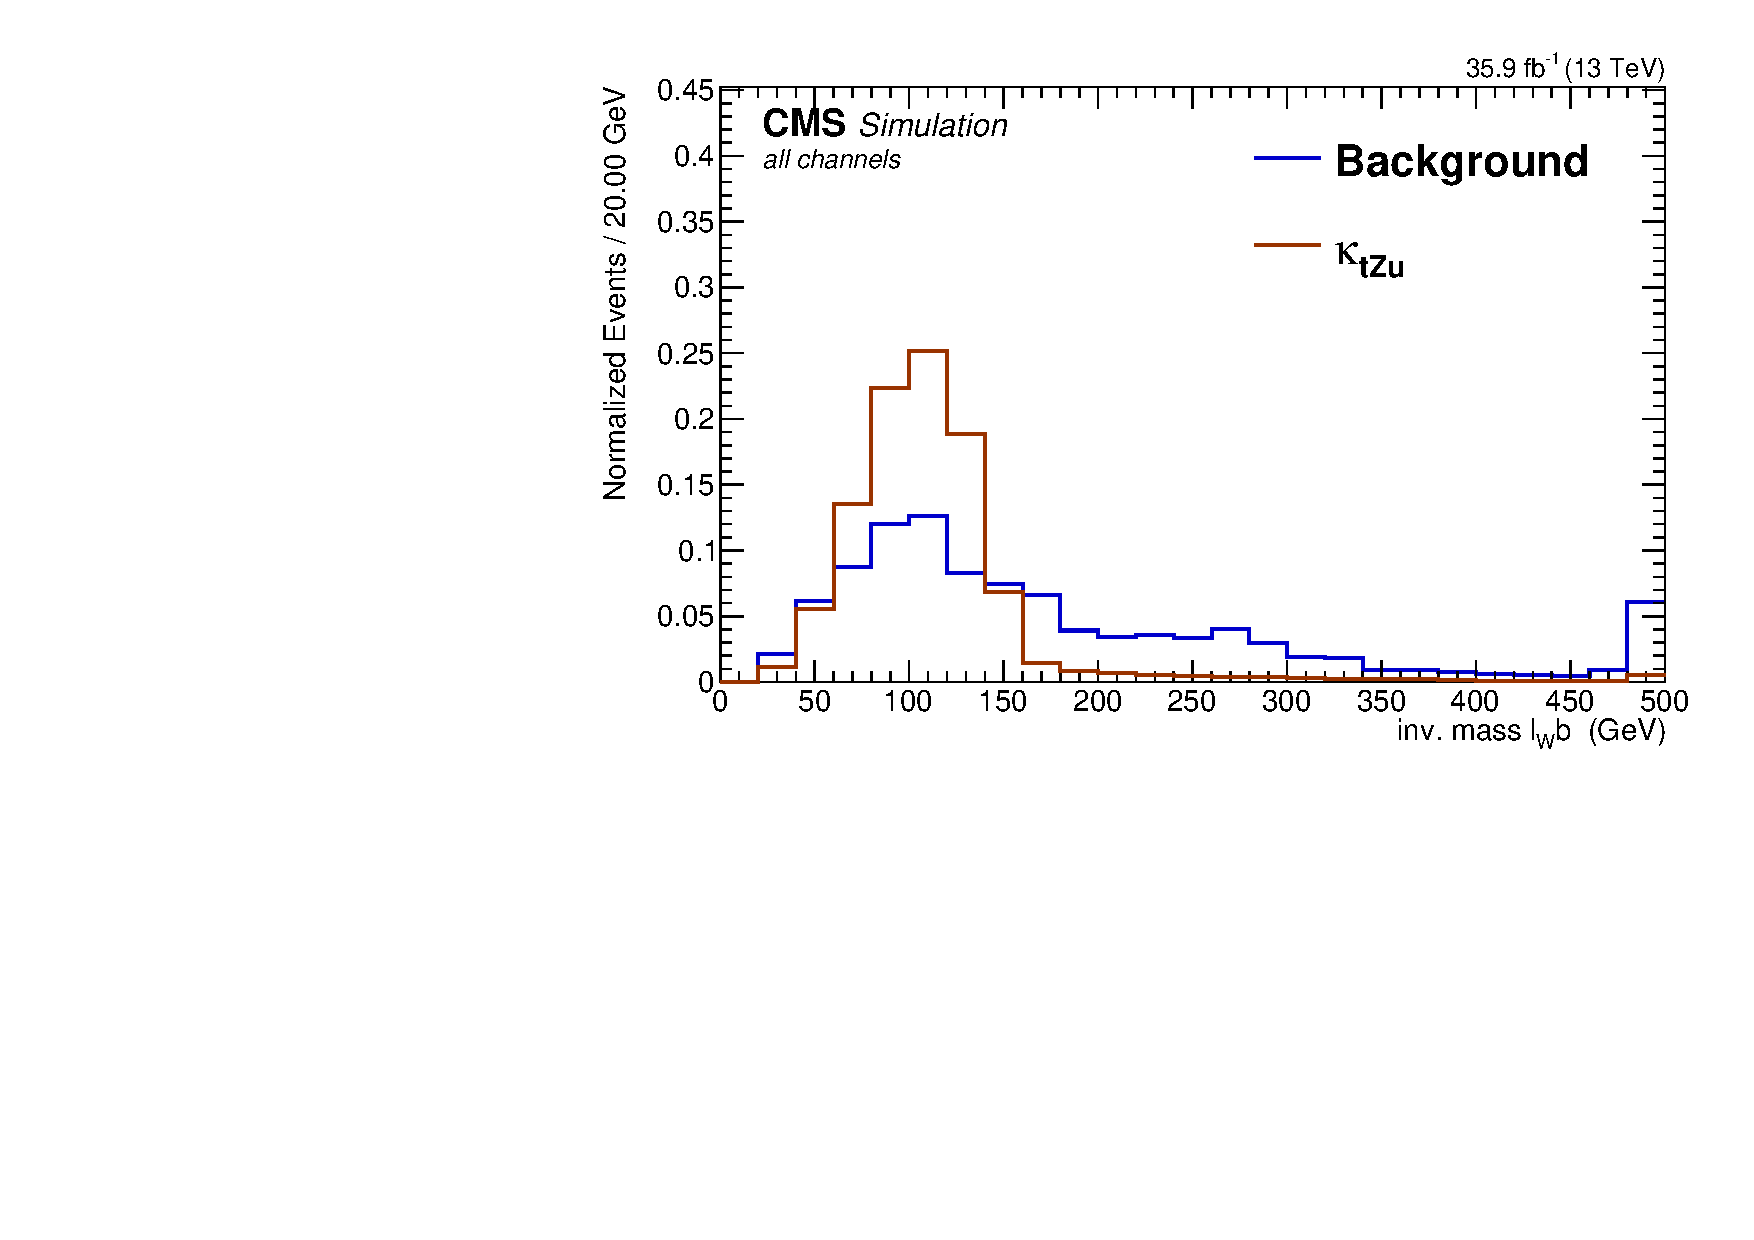
\includegraphics[width=0.3\linewidth]{6_Search/Figures/BDTinputvars/Zut/toppair_MVA_mlb_all_Normalized}
	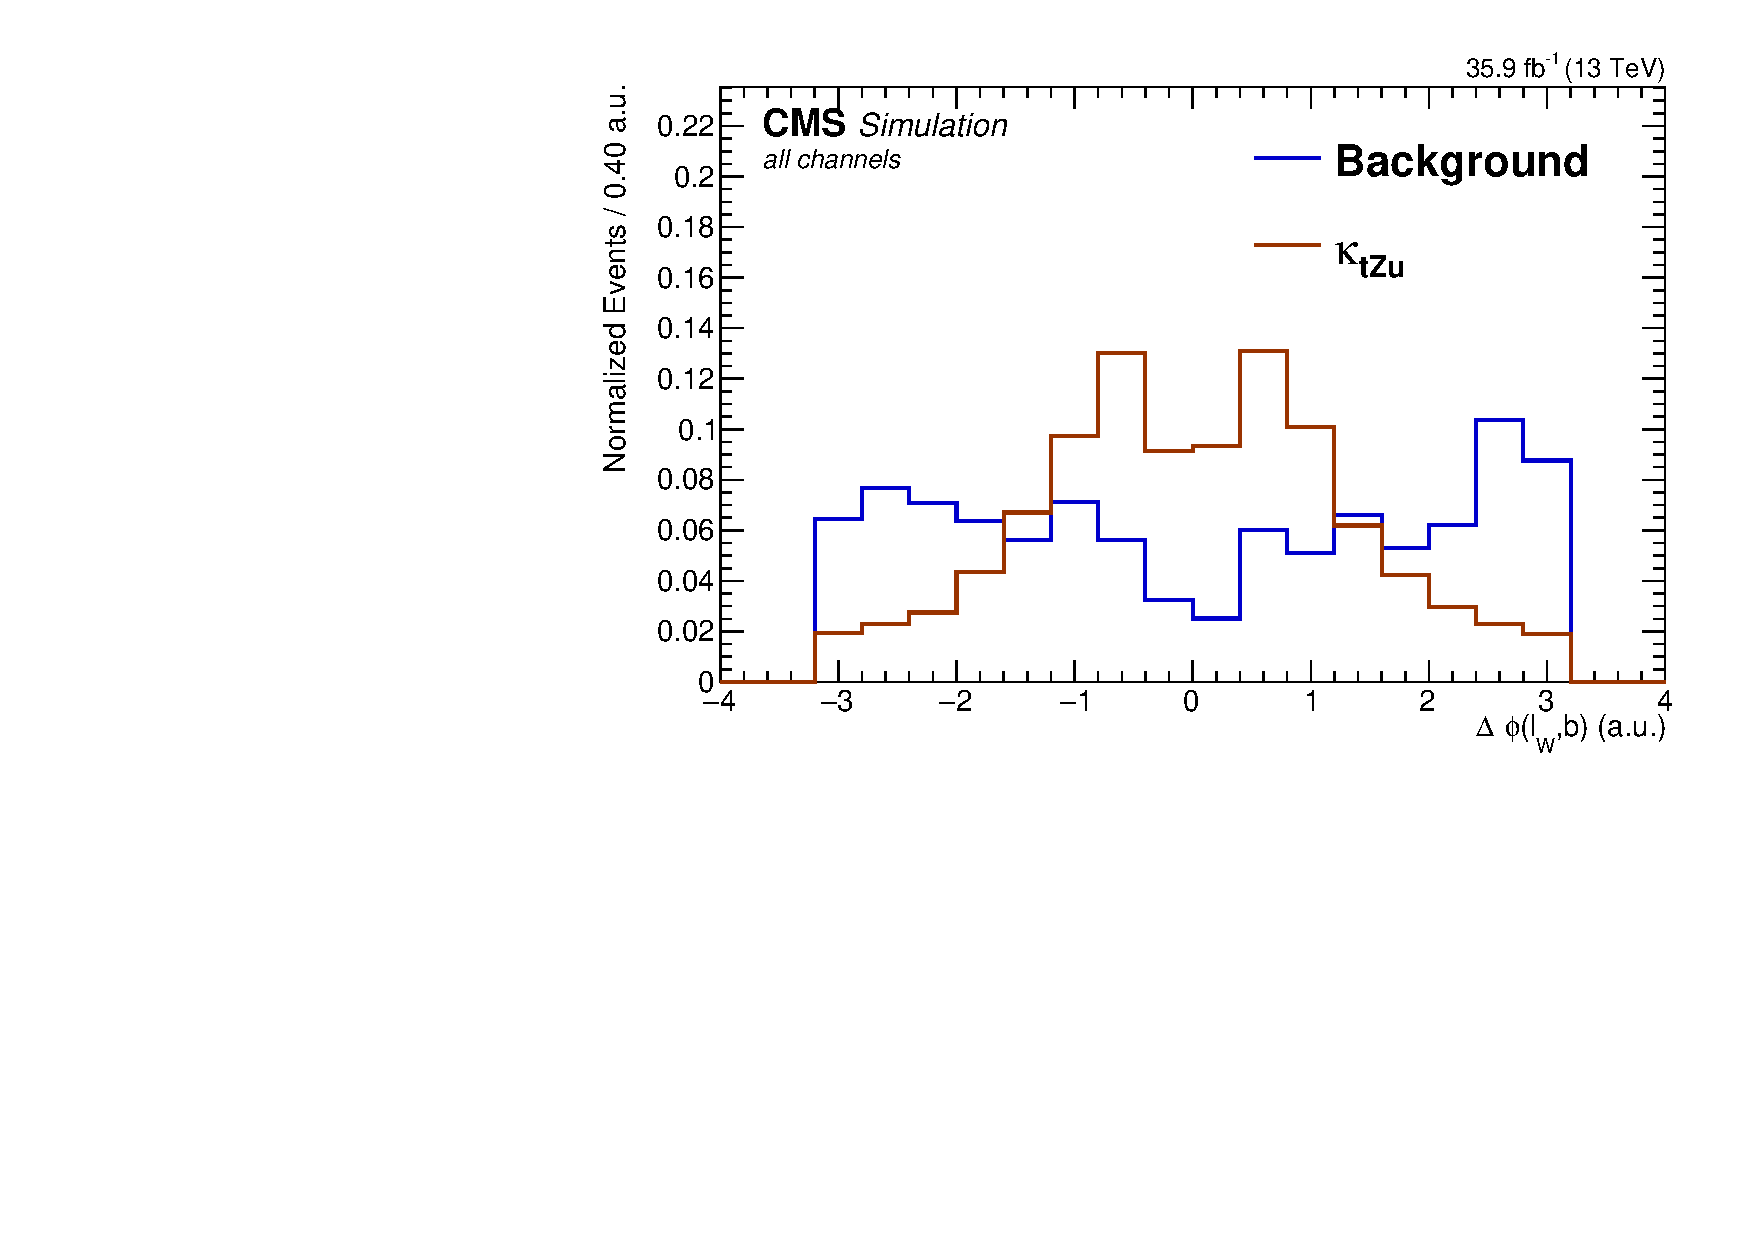
\includegraphics[width=0.3\linewidth]{6_Search/Figures/BDTinputvars/Zut/toppair_MVA_dPhiWlepb_all_Normalized}
	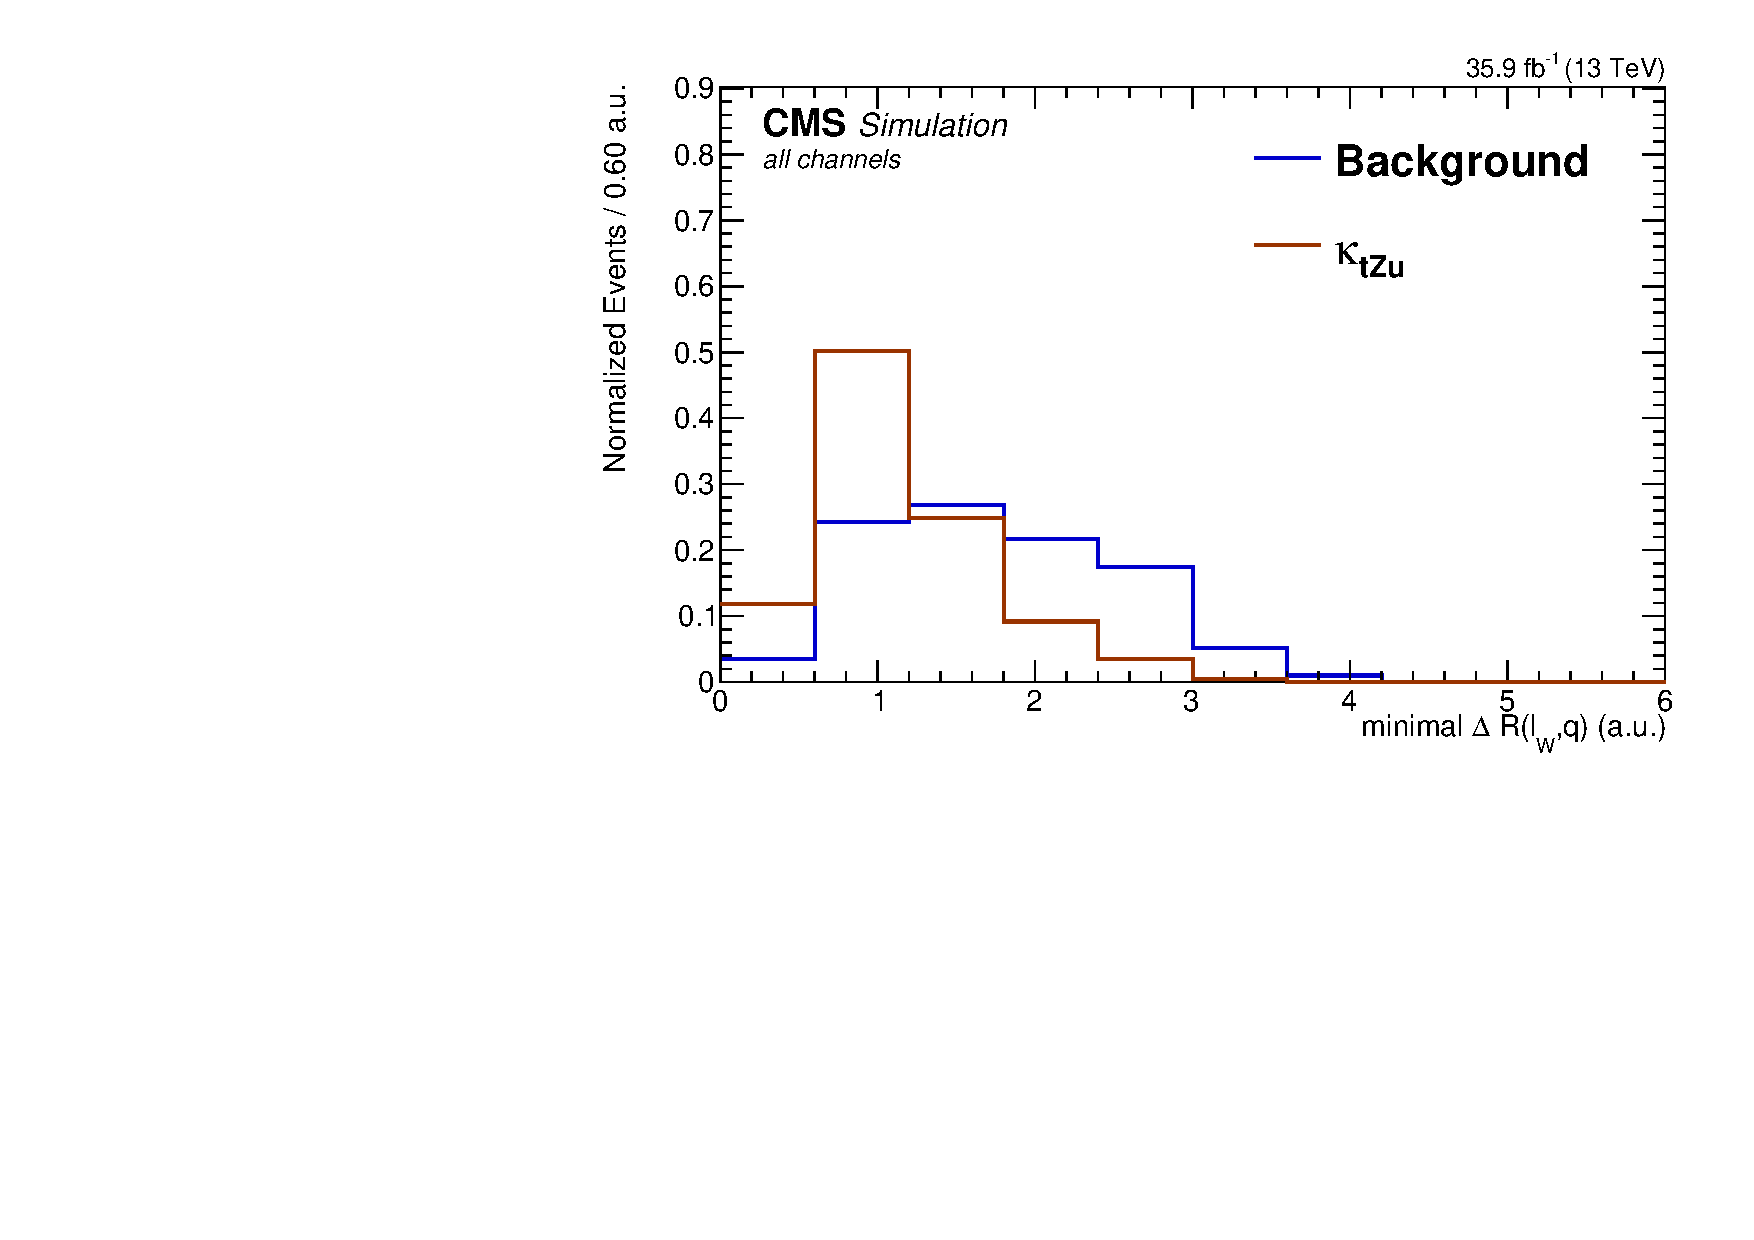
\includegraphics[width=0.3\linewidth]{6_Search/Figures/BDTinputvars/Zut/toppair_MVA_deltaRWlepJet_min_all_Normalized}
	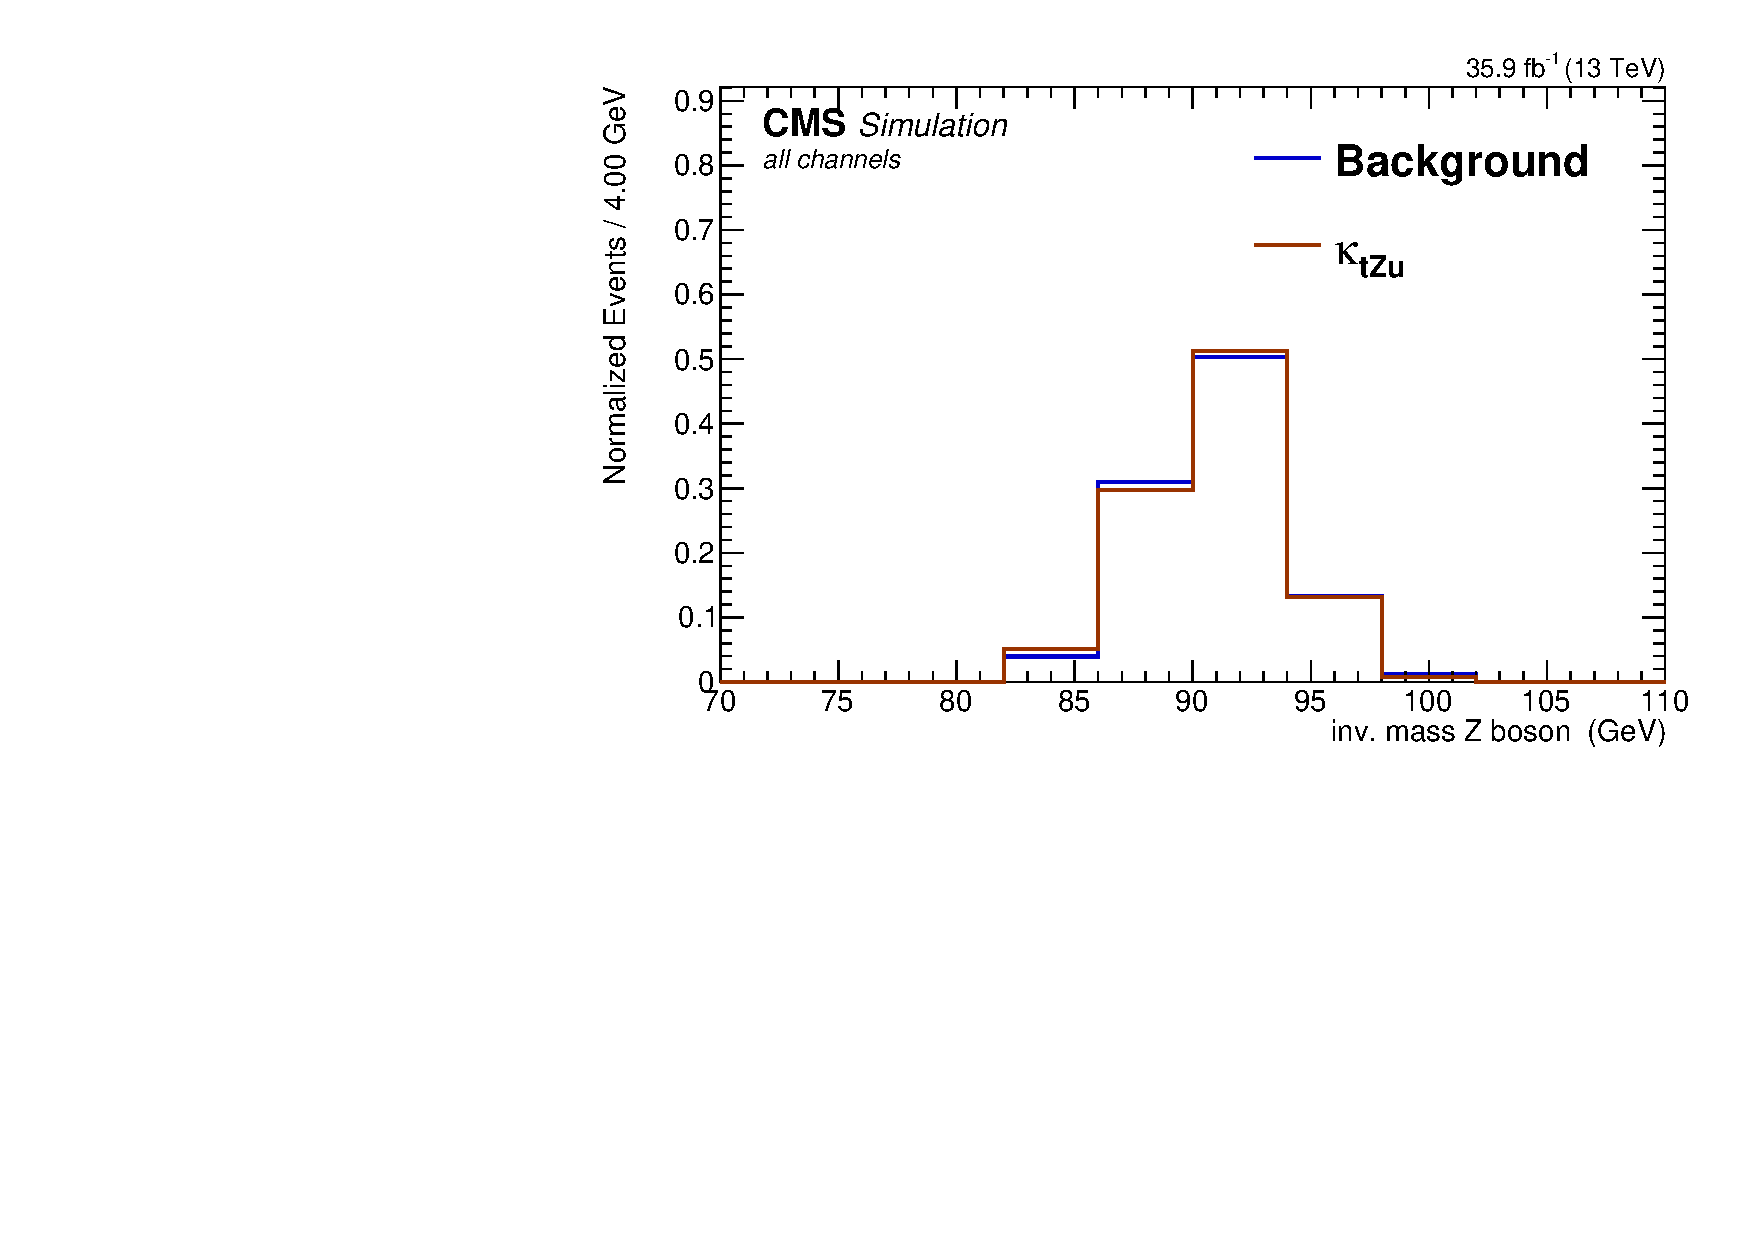
\includegraphics[width=0.3\linewidth]{6_Search/Figures/BDTinputvars/Zut/toppair_MVA_Zboson_M_all_Normalized}
	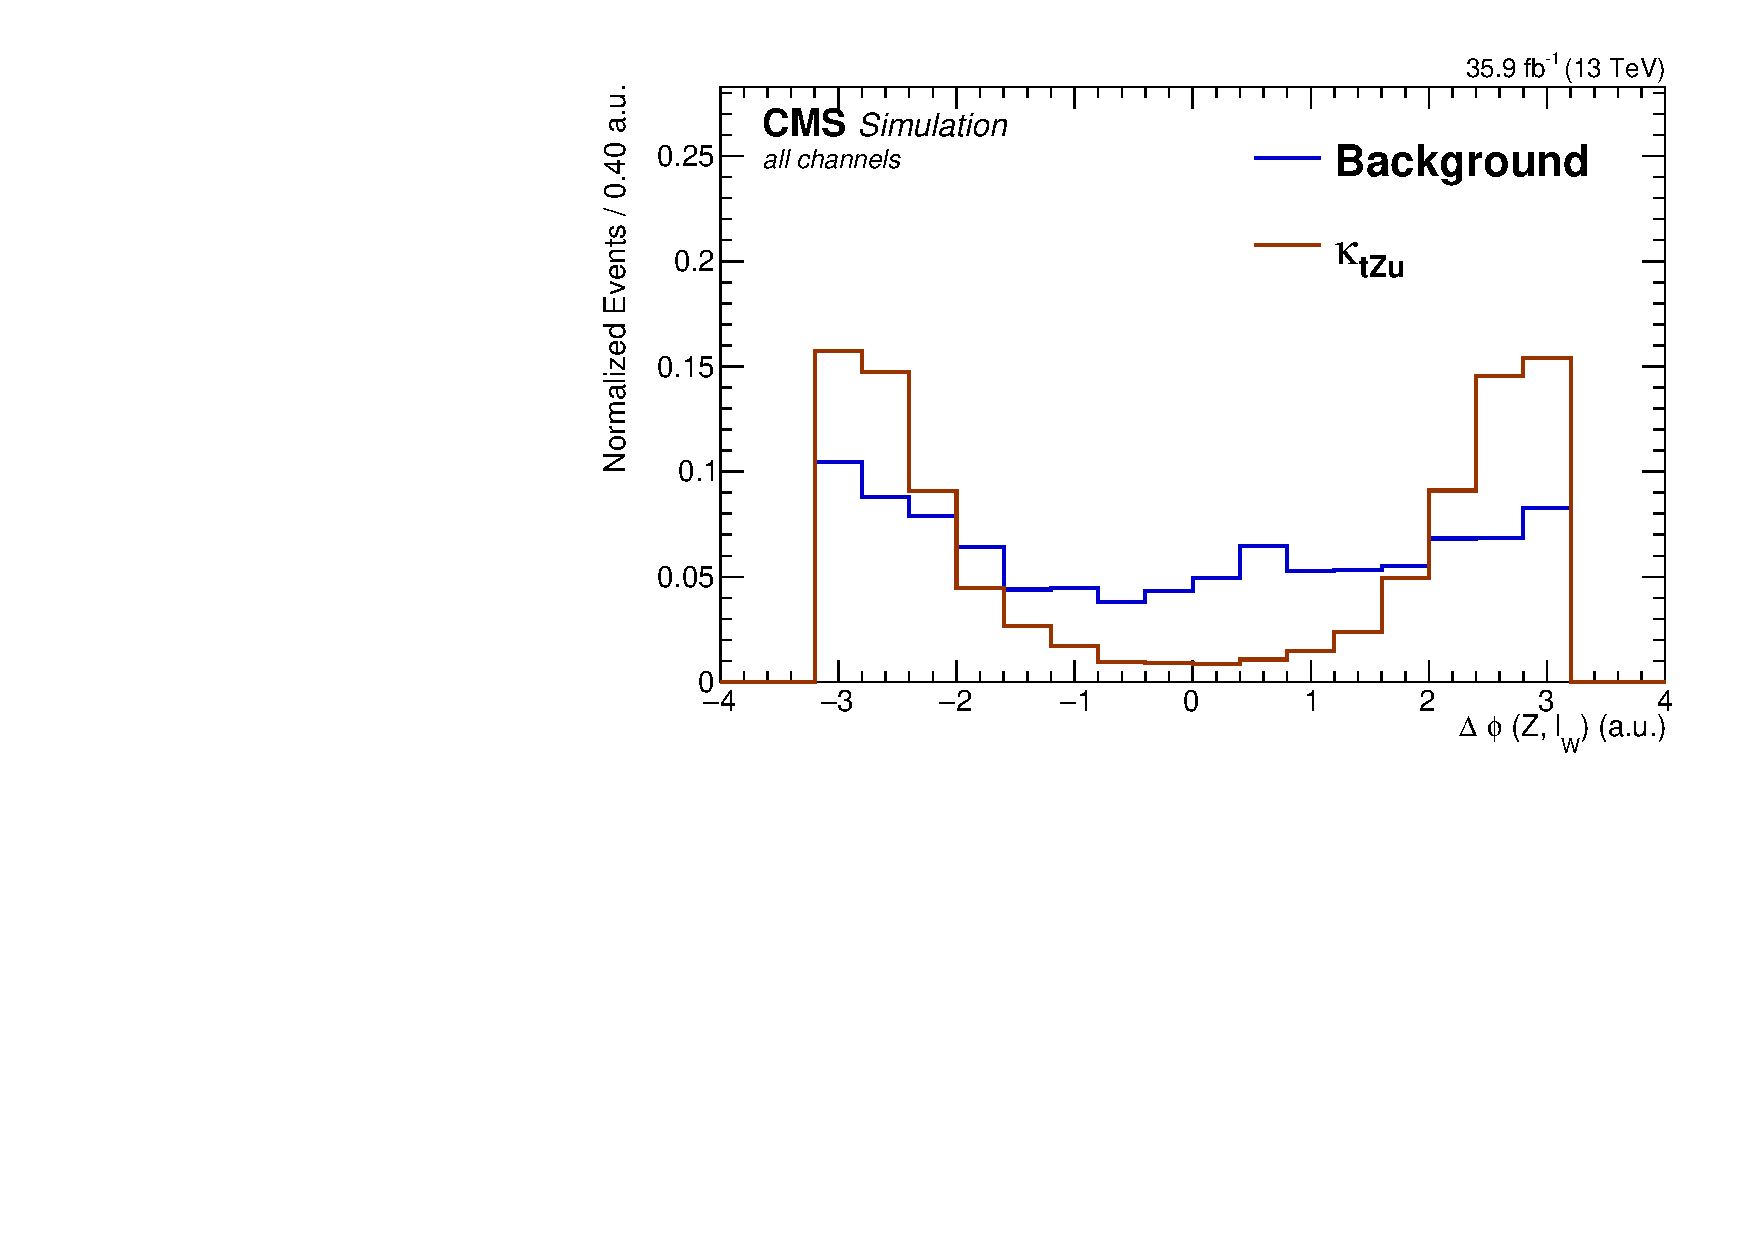
\includegraphics[width=0.3\linewidth]{6_Search/Figures/BDTinputvars/Zut/toppair_MVA_dPhiZWlep_all_Normalized}
	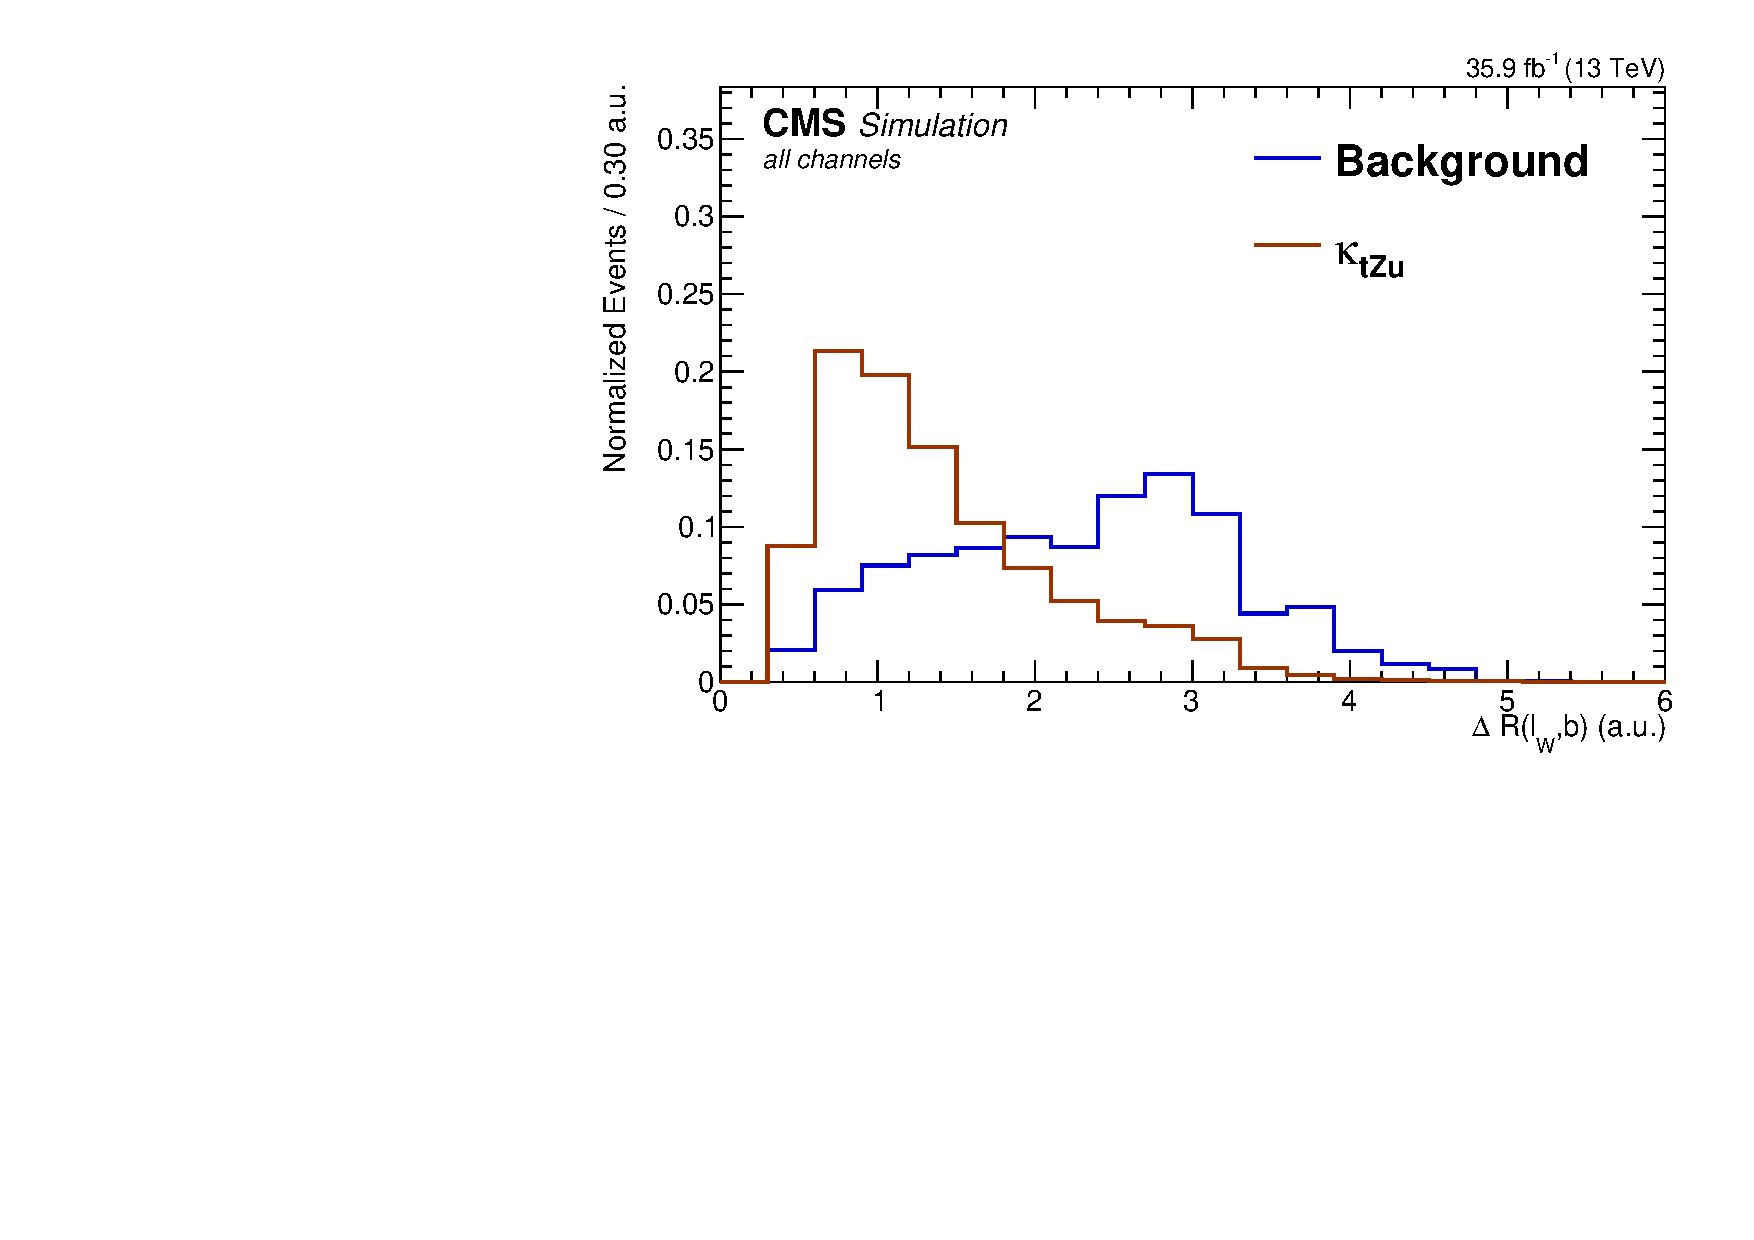
\includegraphics[width=0.3\linewidth]{6_Search/Figures/BDTinputvars/Zut/toppair_MVA_dRWlepb_all_Normalized}
	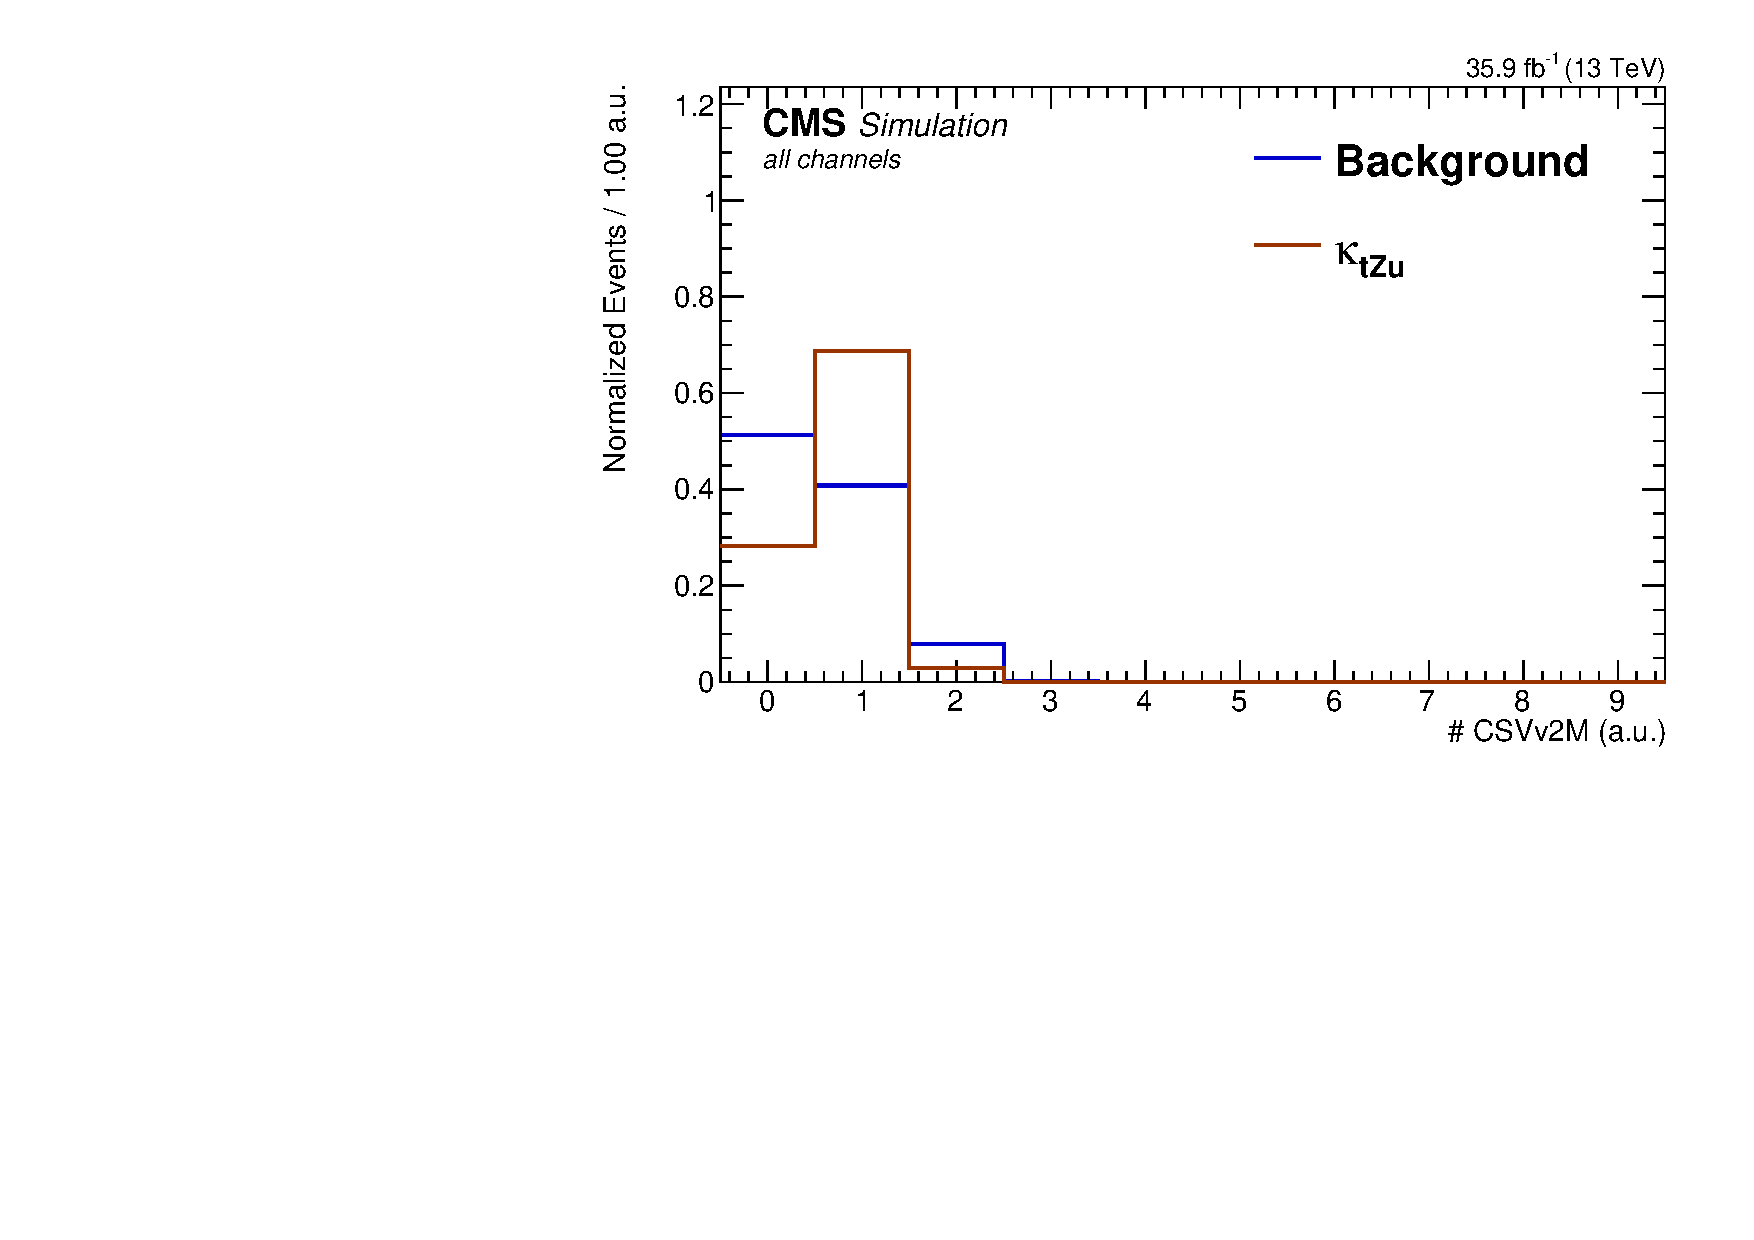
\includegraphics[width=0.3\linewidth]{6_Search/Figures/BDTinputvars/Zut/toppair_MVA_NJets_CSVv2M_all_Normalized}
	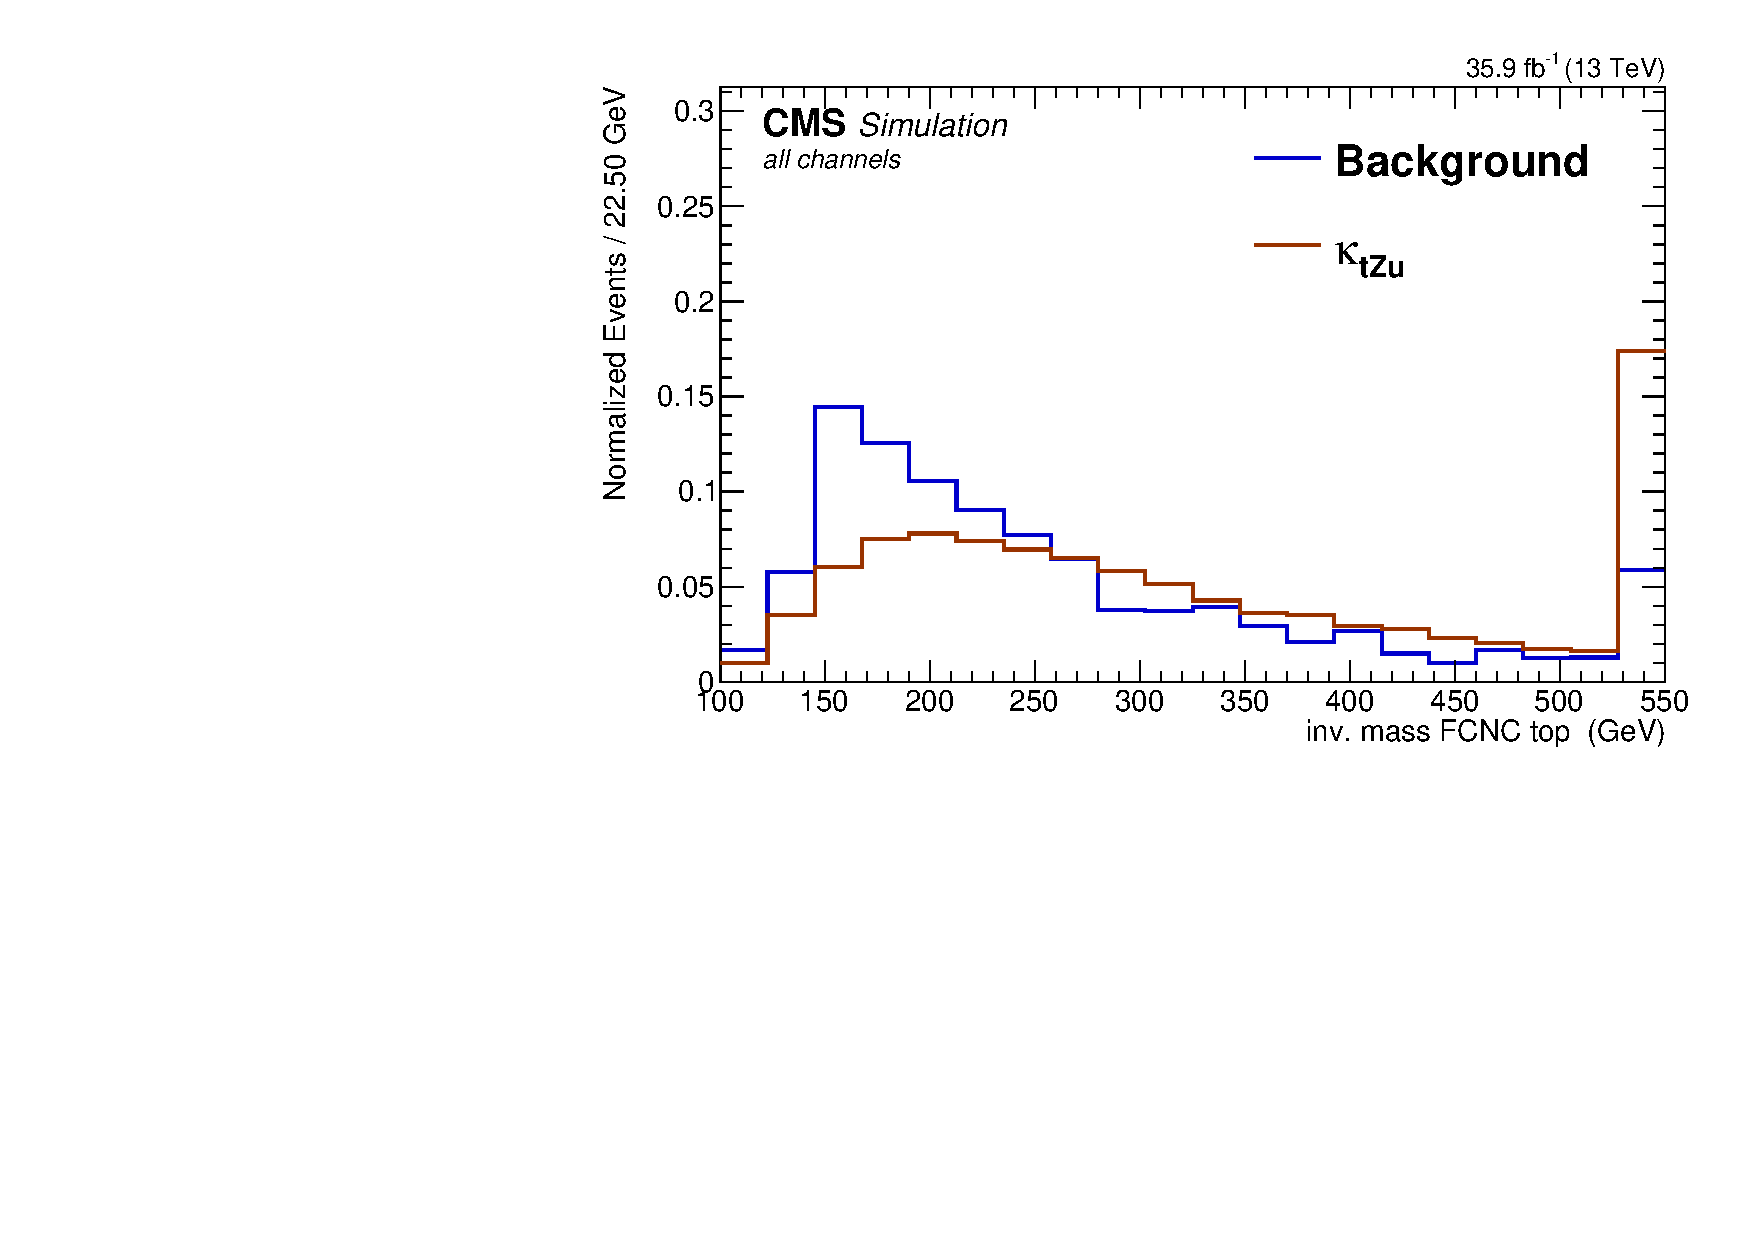
\includegraphics[width=0.3\linewidth]{6_Search/Figures/BDTinputvars/Zut/toppair_MVA_FCNCtop_M_all_Normalized}
	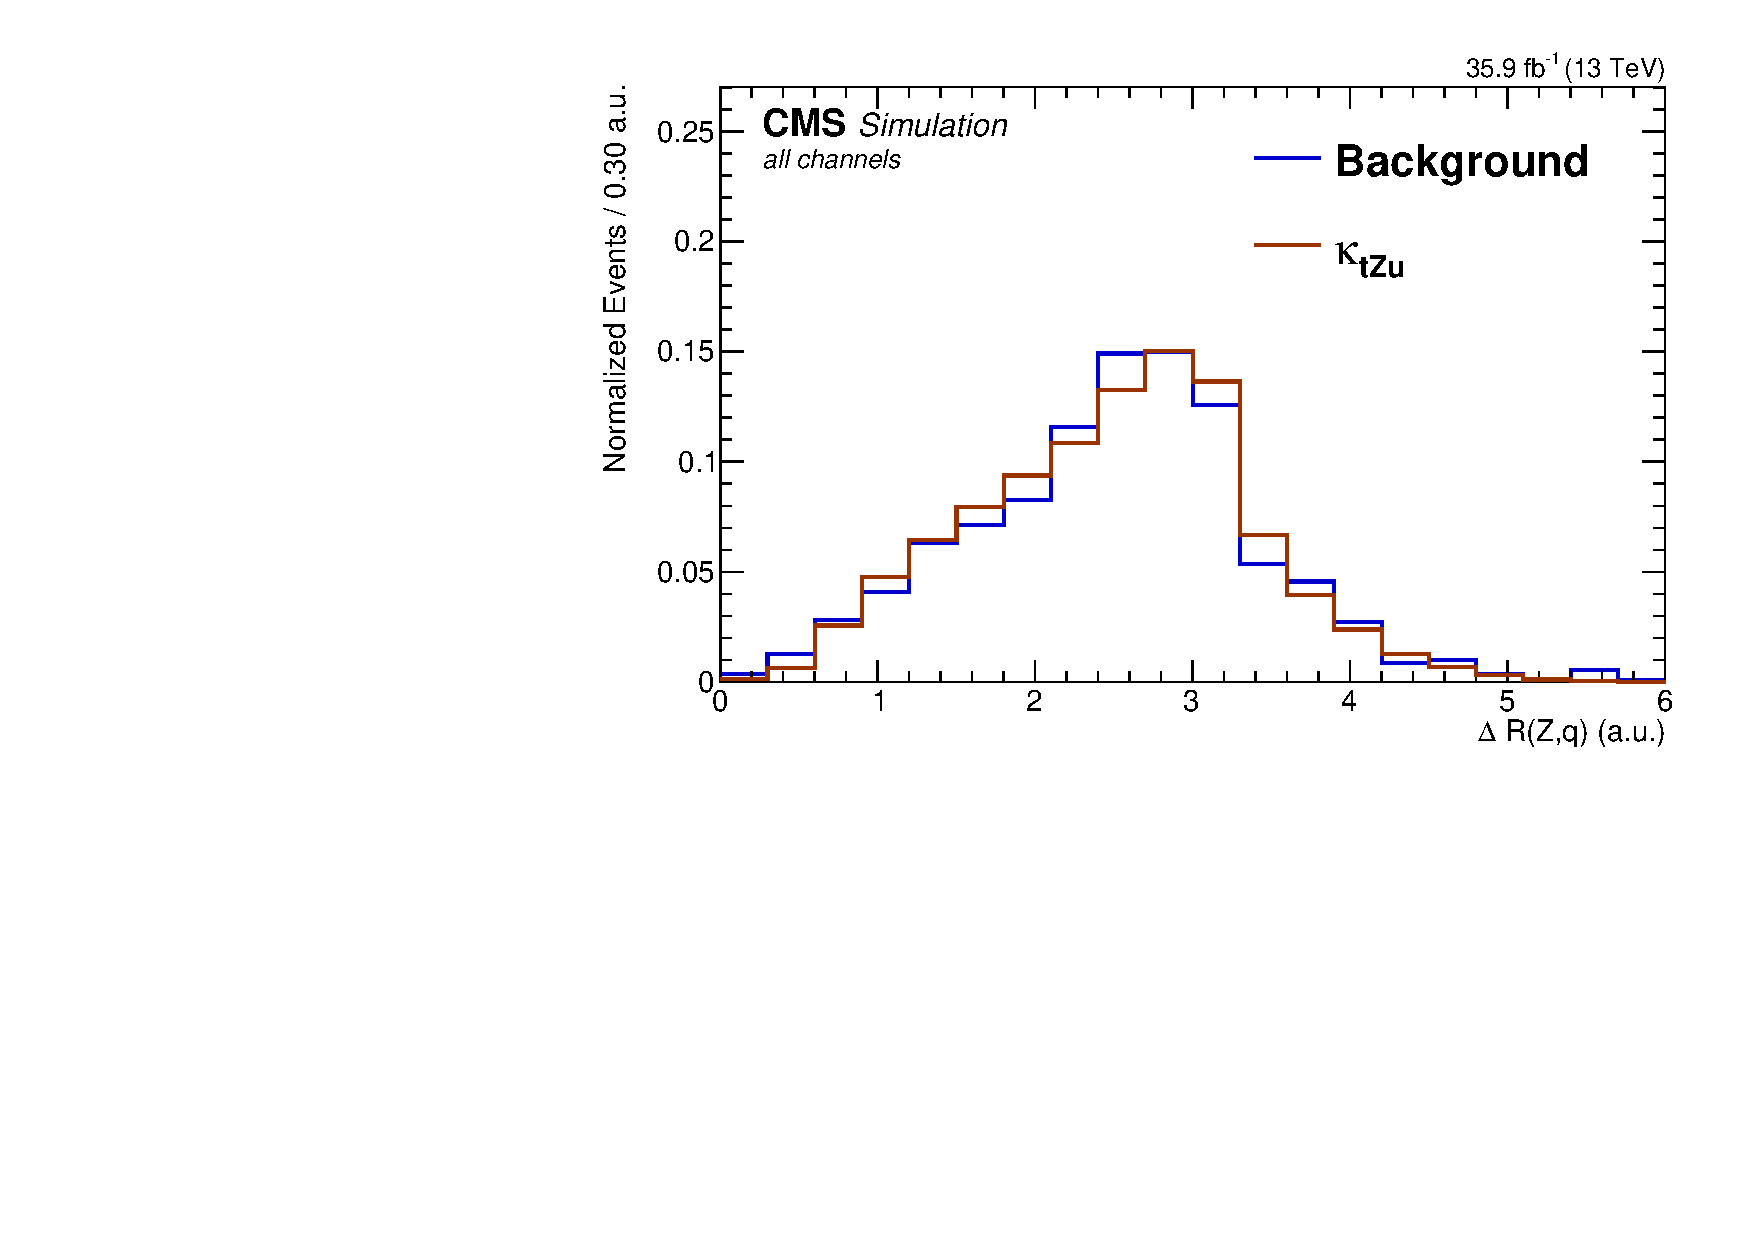
\includegraphics[width=0.3\linewidth]{6_Search/Figures/BDTinputvars/Zut/toppair_MVA_dRZc_all_Normalized}
	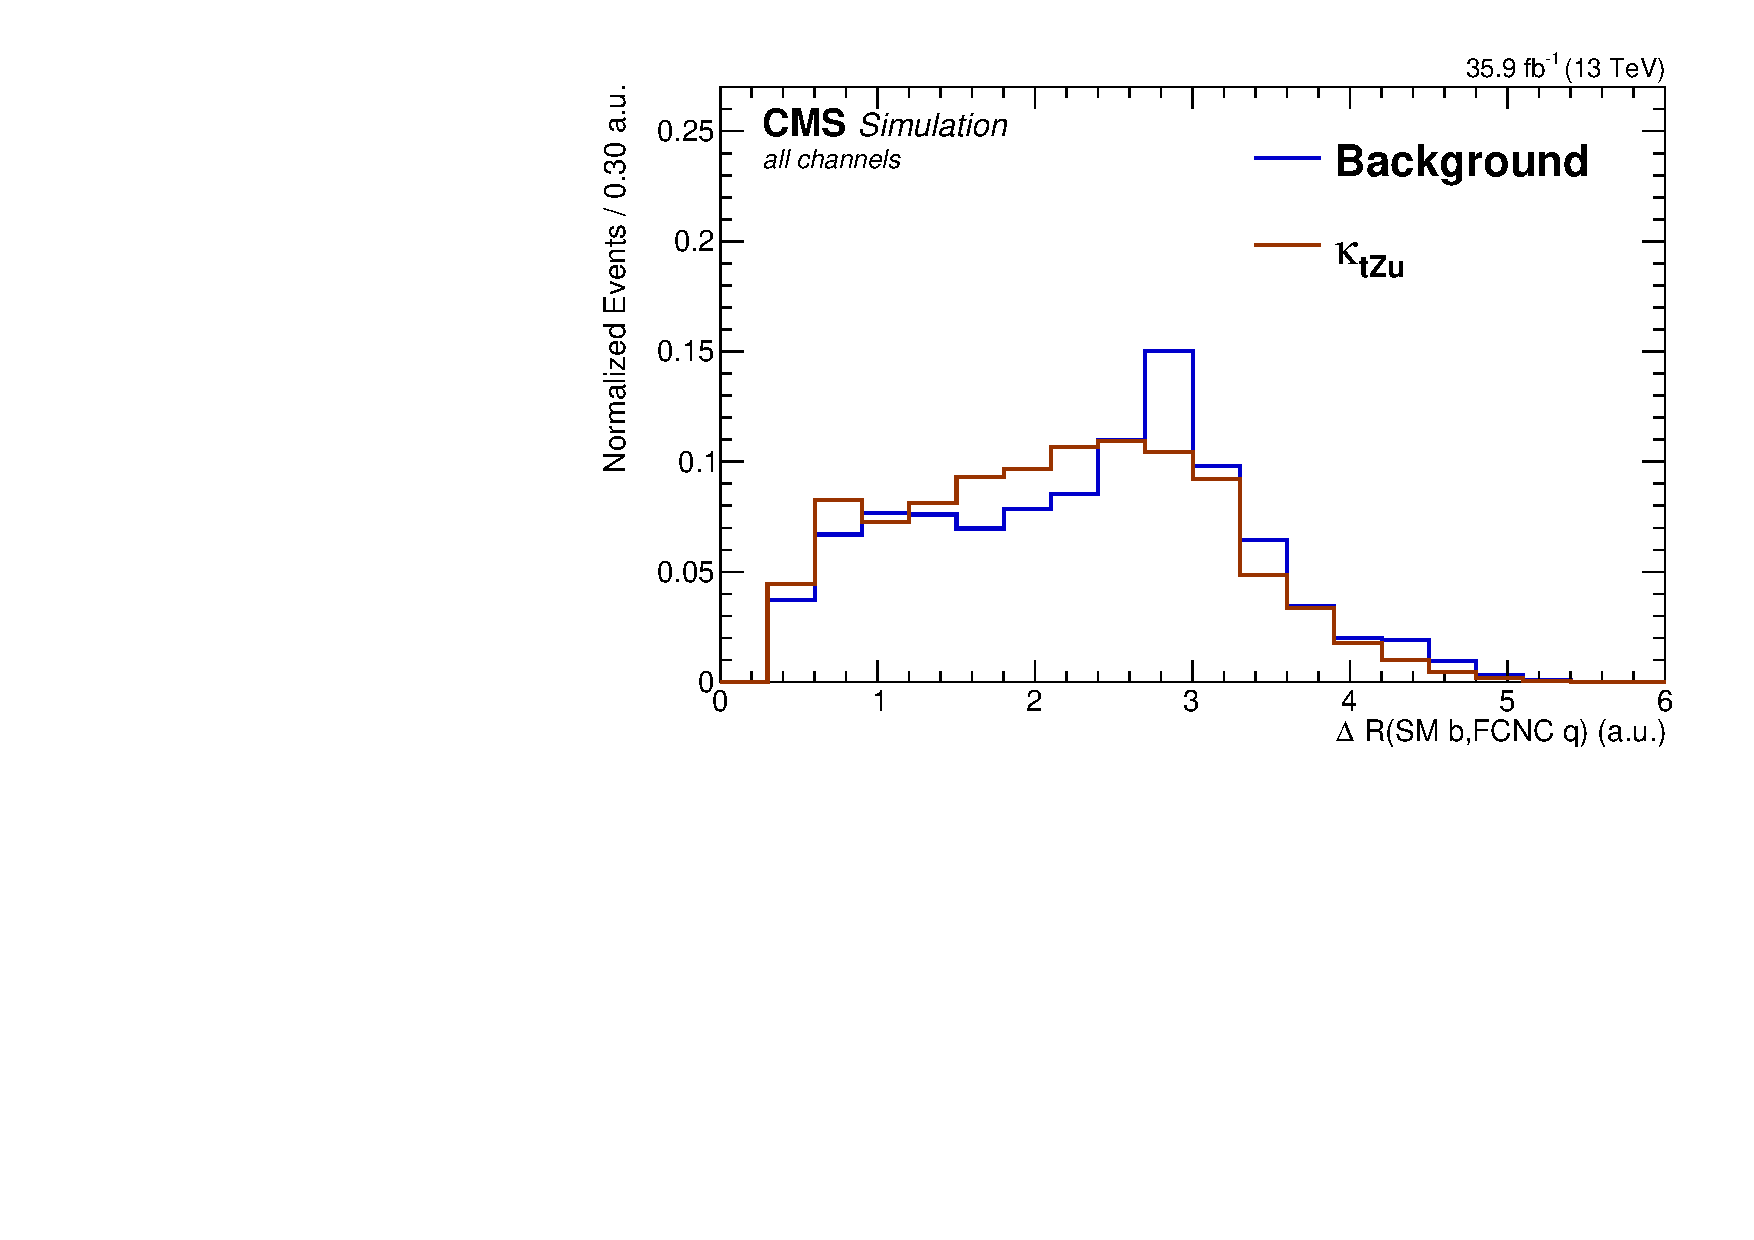
\includegraphics[width=0.3\linewidth]{6_Search/Figures/BDTinputvars/Zut/toppair_MVA_dRSMjetLightjet_all_Normalized}
	\caption{The normalised input variables for reconstructing the multivariate discriminator in the \TTSR\ for the \Zut\ vertex.}
	\label{fig:toppairZutnormalized}
\end{figure}

\begin{figure}[htbp]
	\centering
	\includegraphics[width=0.3\linewidth]{6_Search/Figures/BDTinputvars/Zut/singletop_MVA_SMtop_Eta_all_Normalized}
	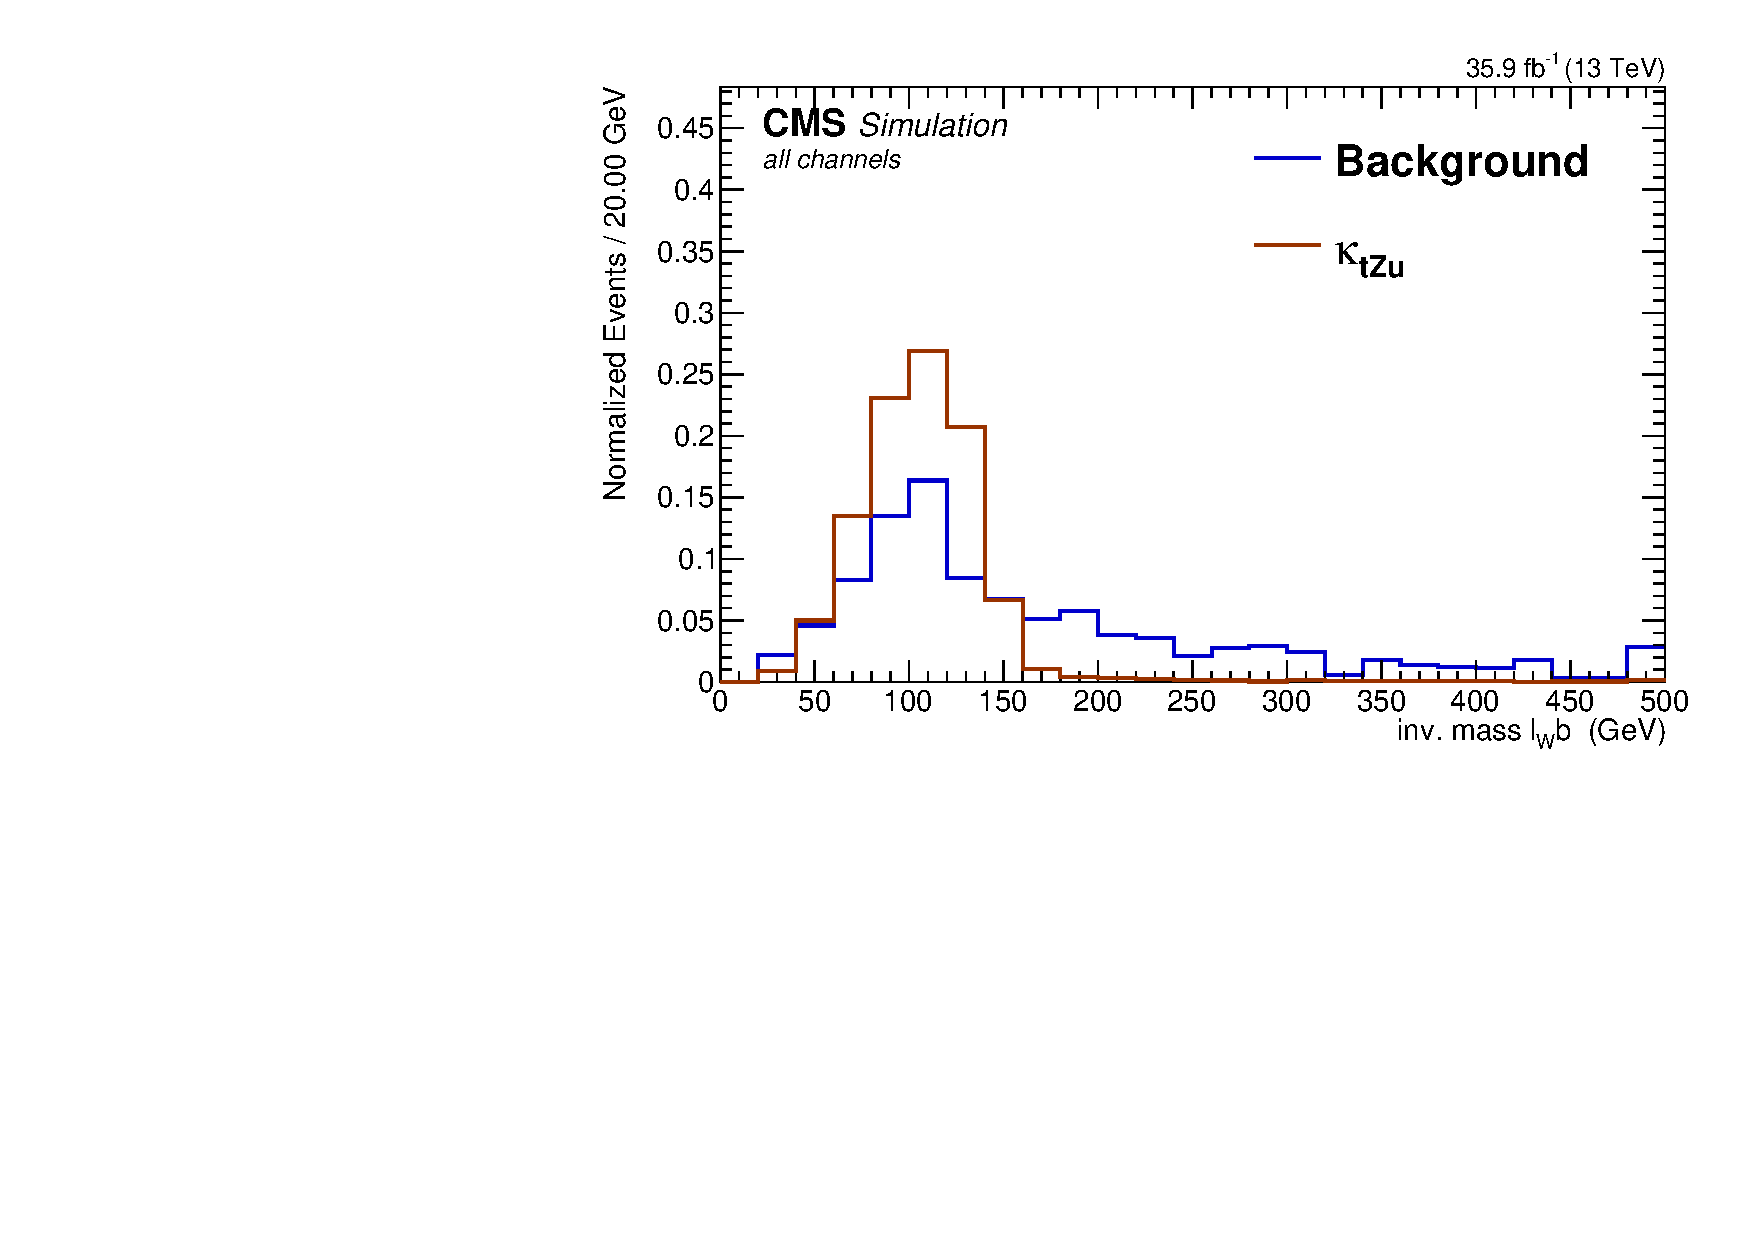
\includegraphics[width=0.3\linewidth]{6_Search/Figures/BDTinputvars/Zut/singletop_MVA_mlb_all_Normalized}
	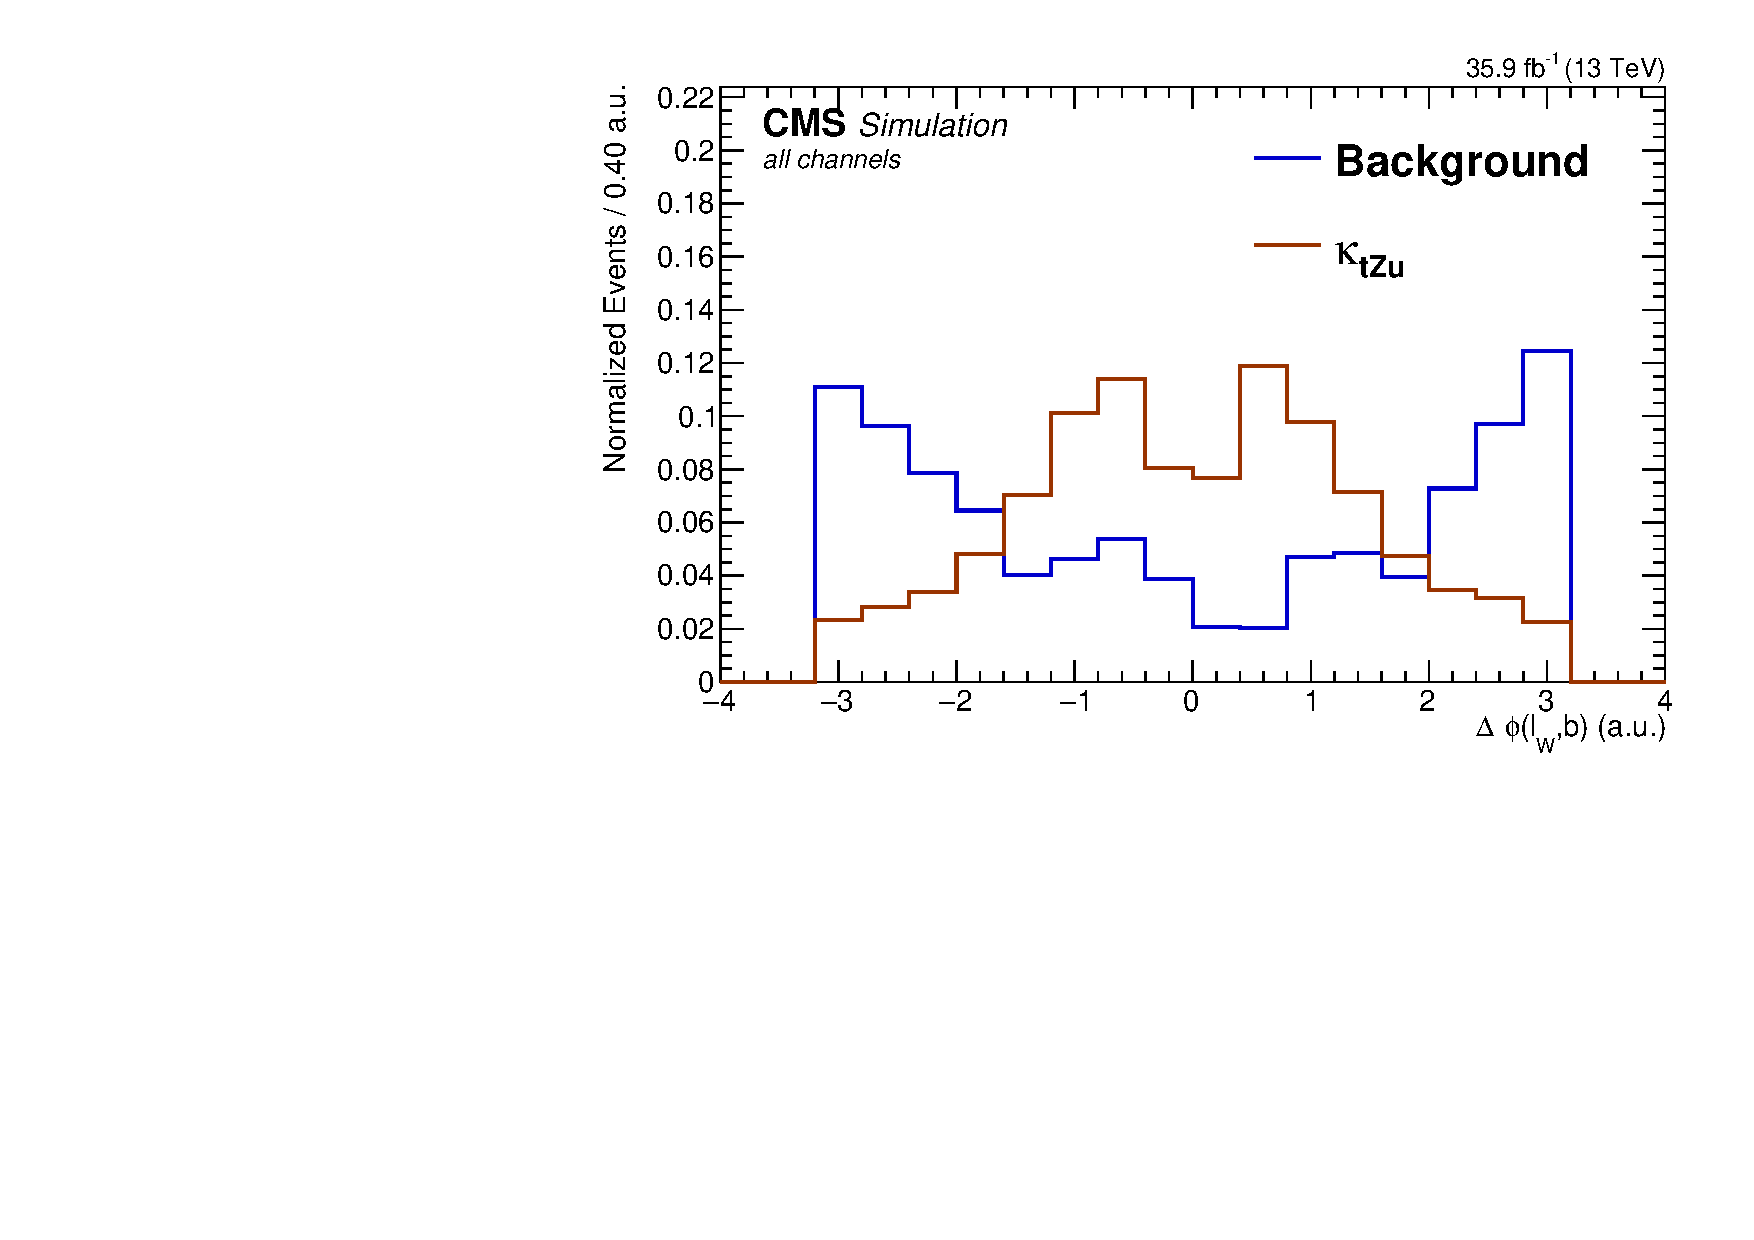
\includegraphics[width=0.3\linewidth]{6_Search/Figures/BDTinputvars/Zut/singletop_MVA_dPhiWlepb_all_Normalized}
	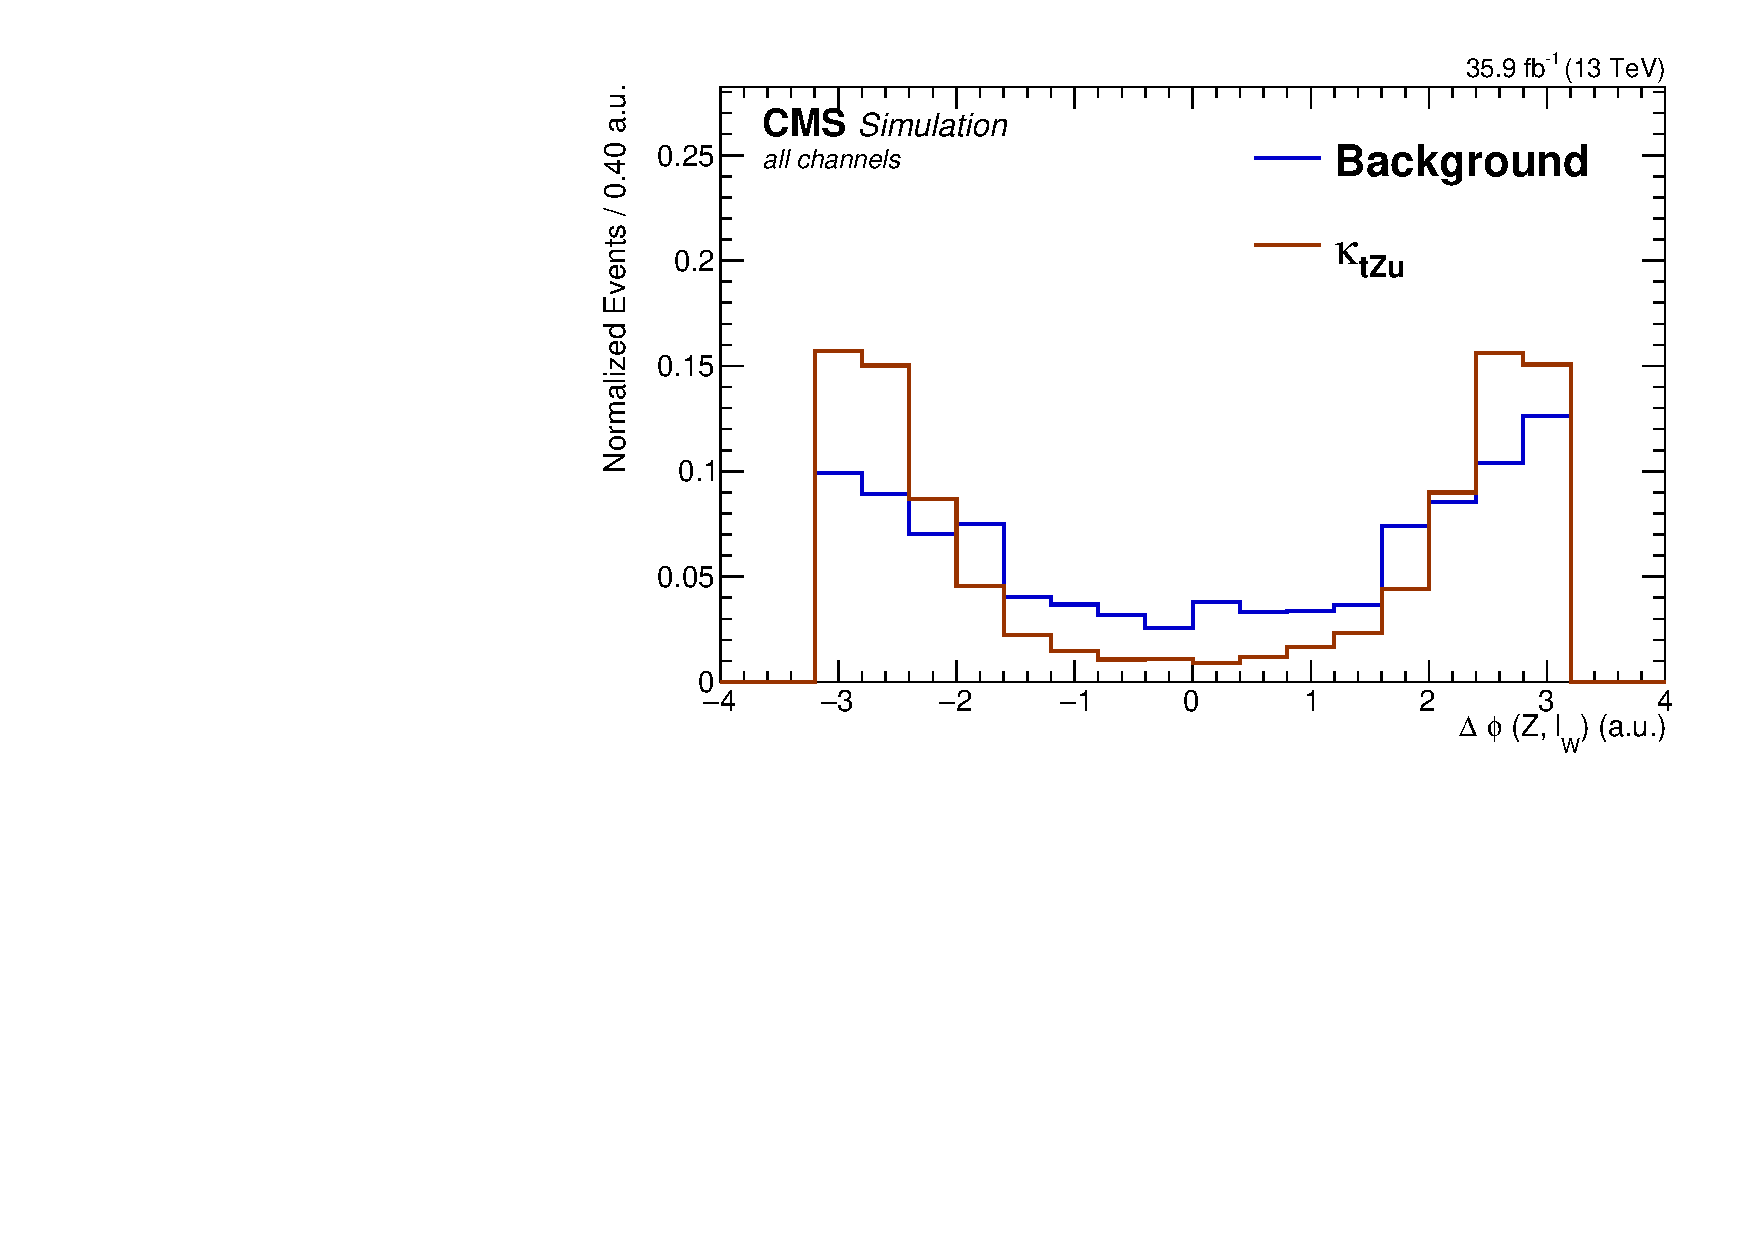
\includegraphics[width=0.3\linewidth]{6_Search/Figures/BDTinputvars/Zut/singletop_MVA_dPhiZWlep_all_Normalized}
	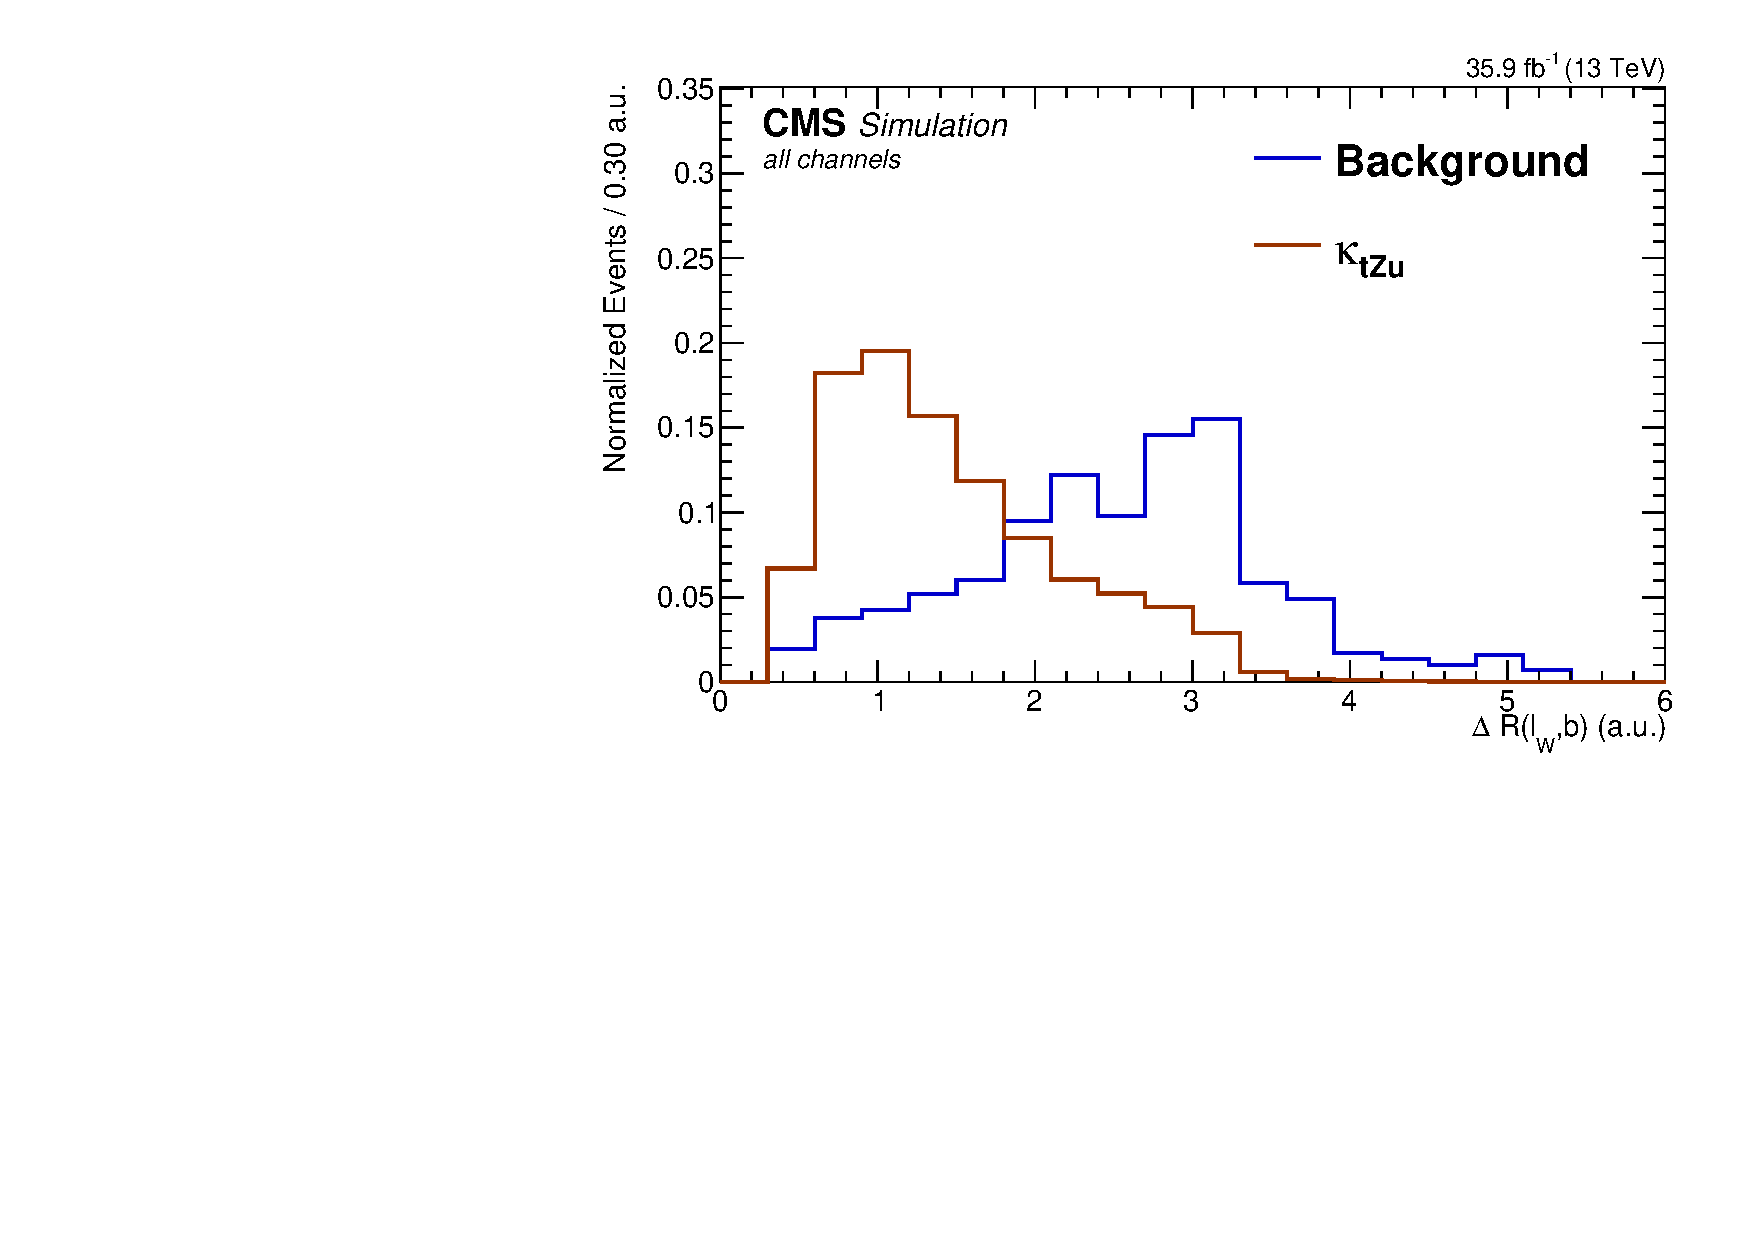
\includegraphics[width=0.3\linewidth]{6_Search/Figures/BDTinputvars/Zut/singletop_MVA_dRWlepb_all_Normalized}
    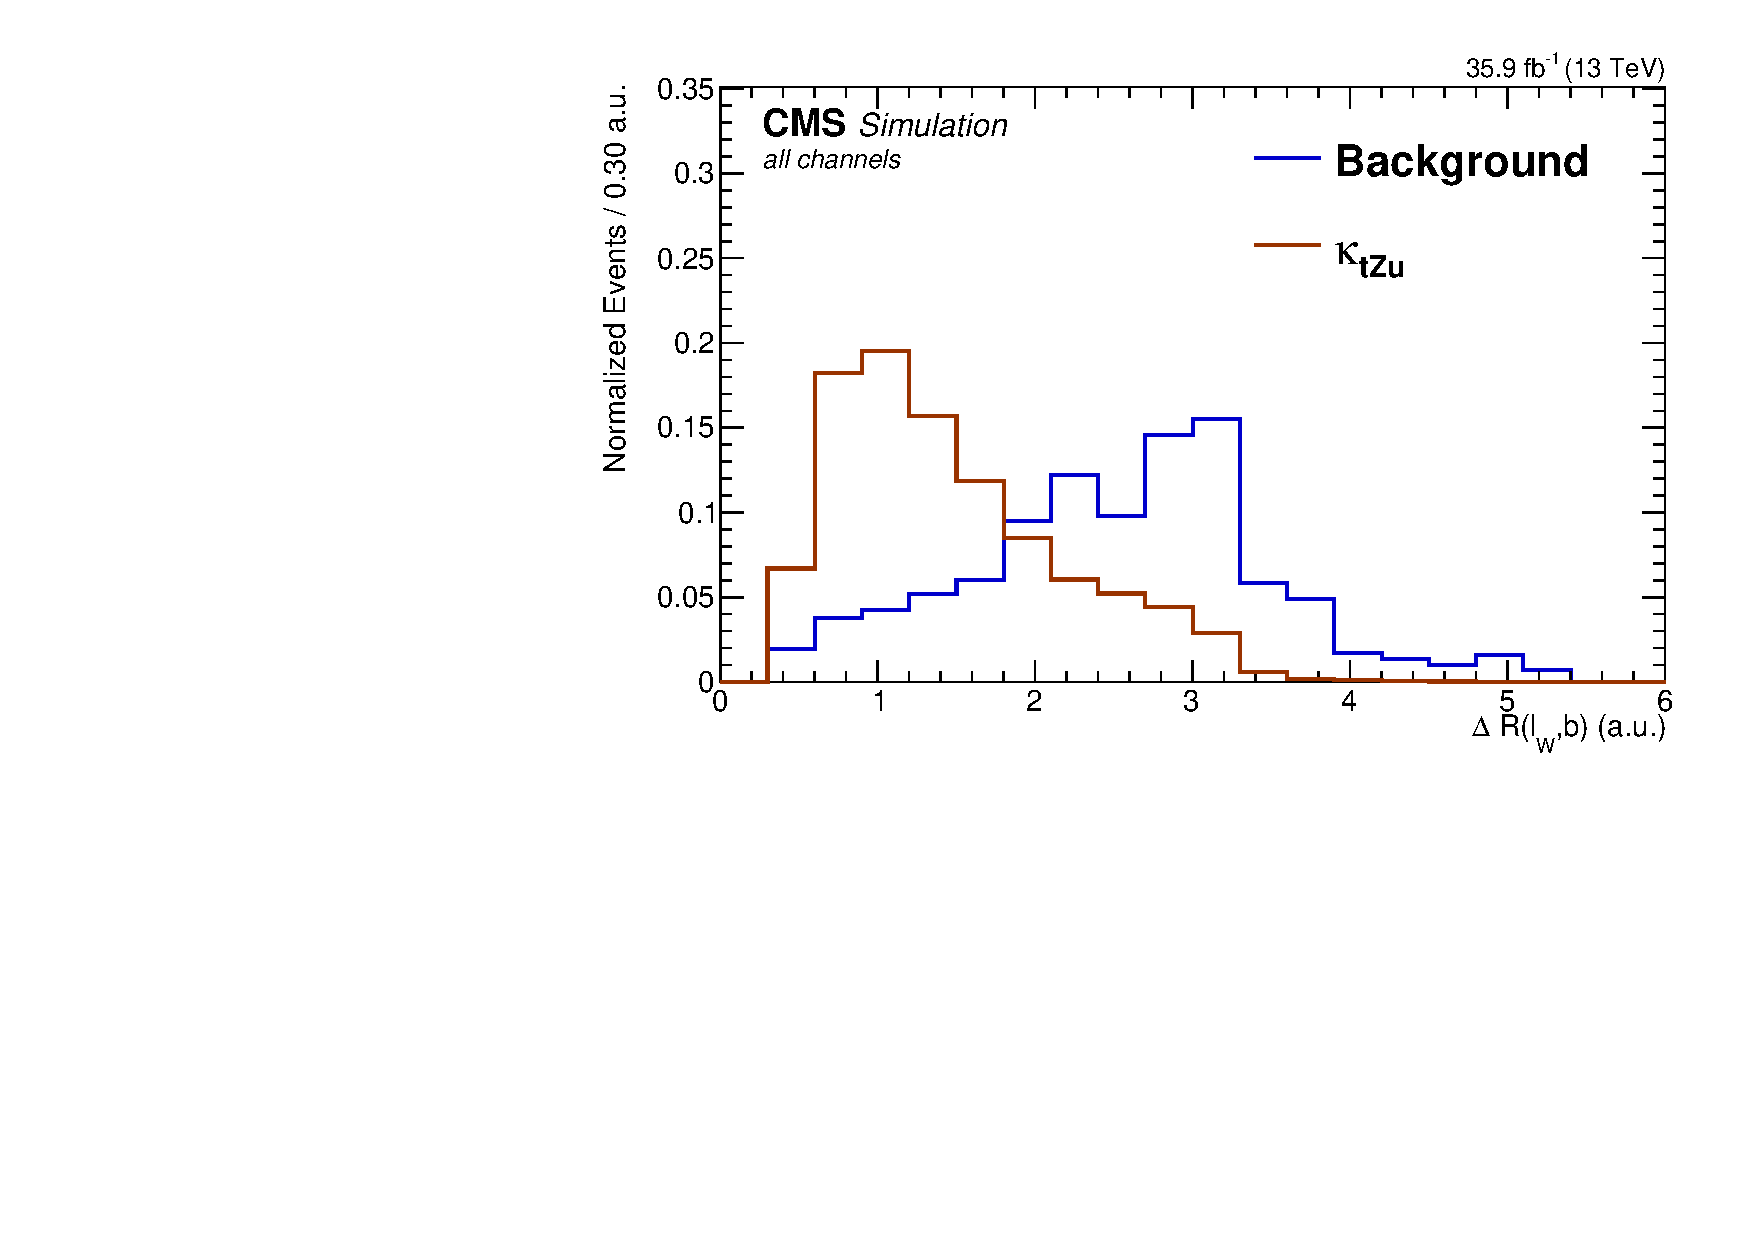
\includegraphics[width=0.3\linewidth]{6_Search/Figures/BDTinputvars/Zut/singletop_MVA_dRWlepb_all_Normalized}
    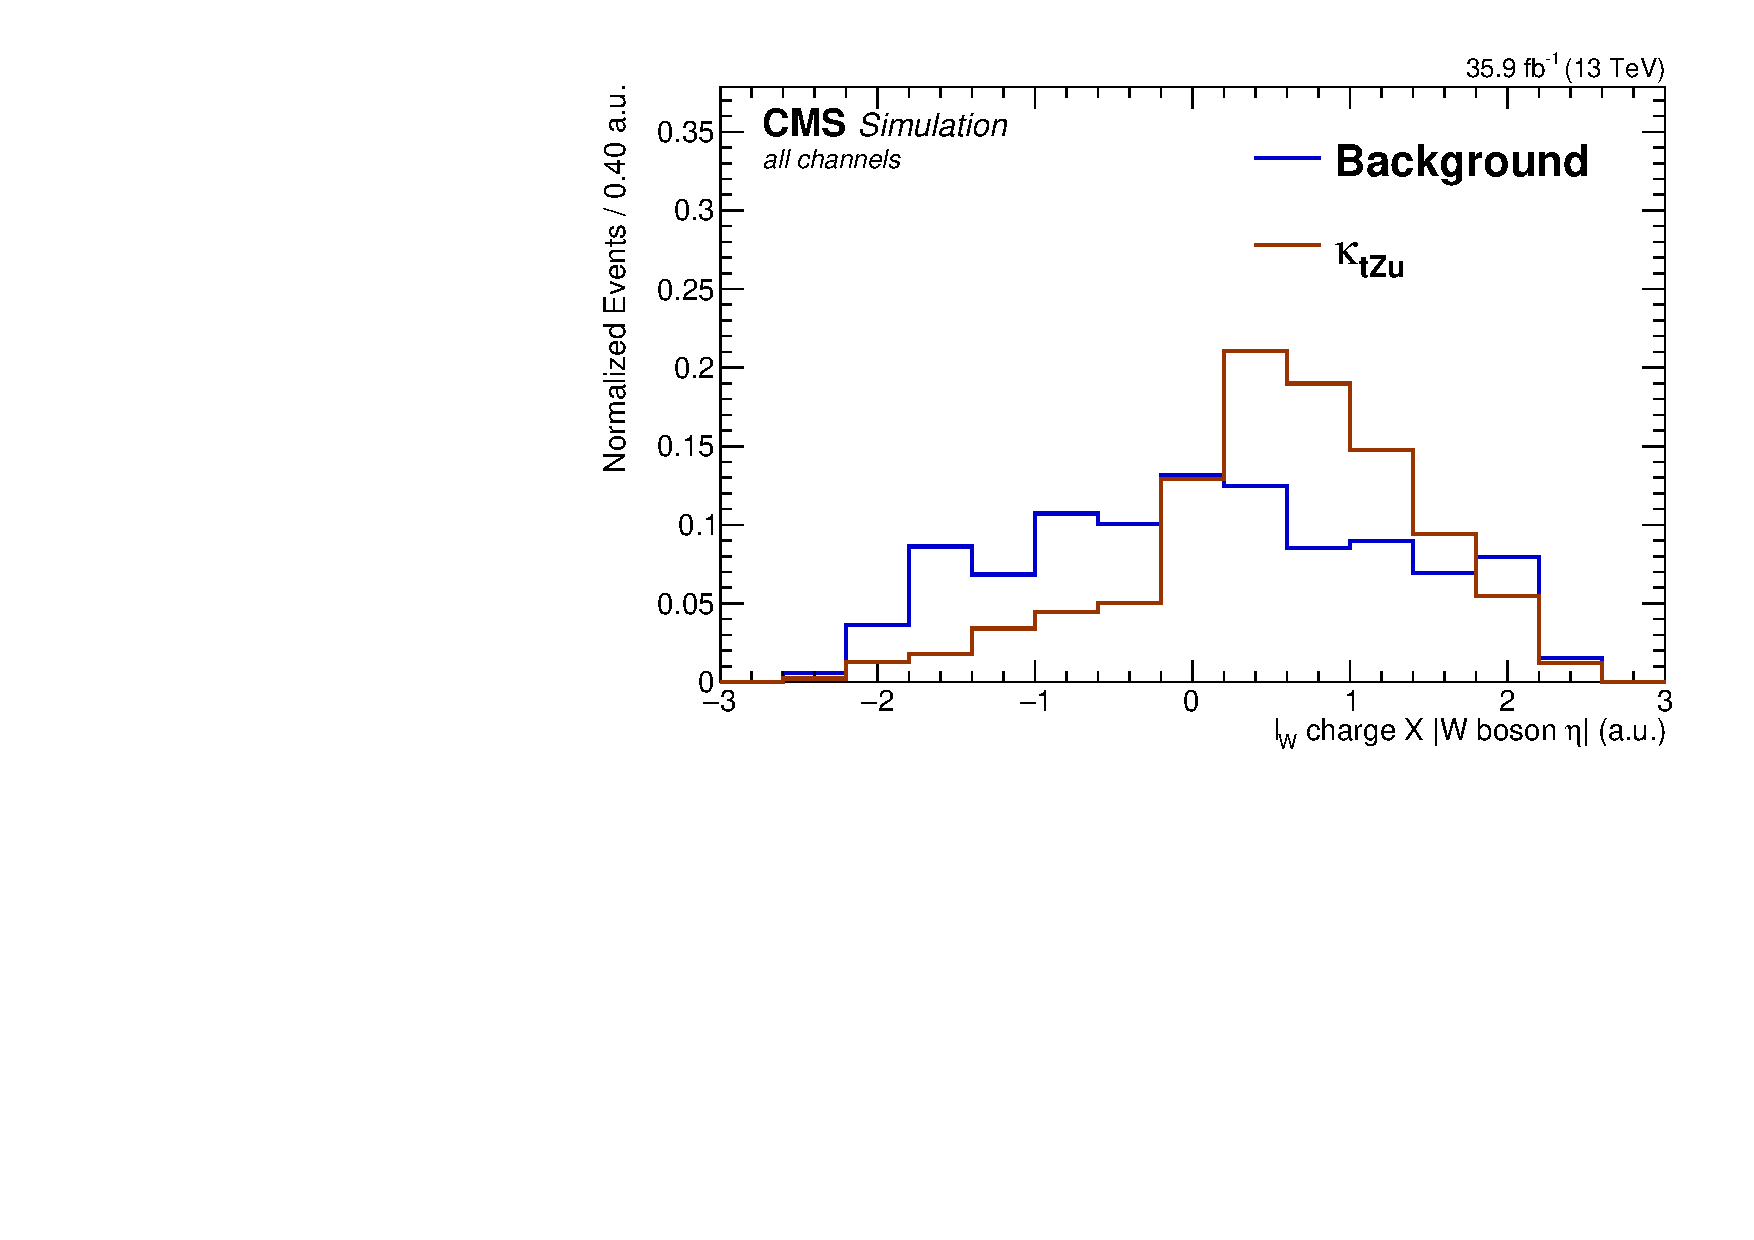
\includegraphics[width=0.3\linewidth]{6_Search/Figures/BDTinputvars/Zut/singletop_MVA_charge_asym_all_Normalized}
    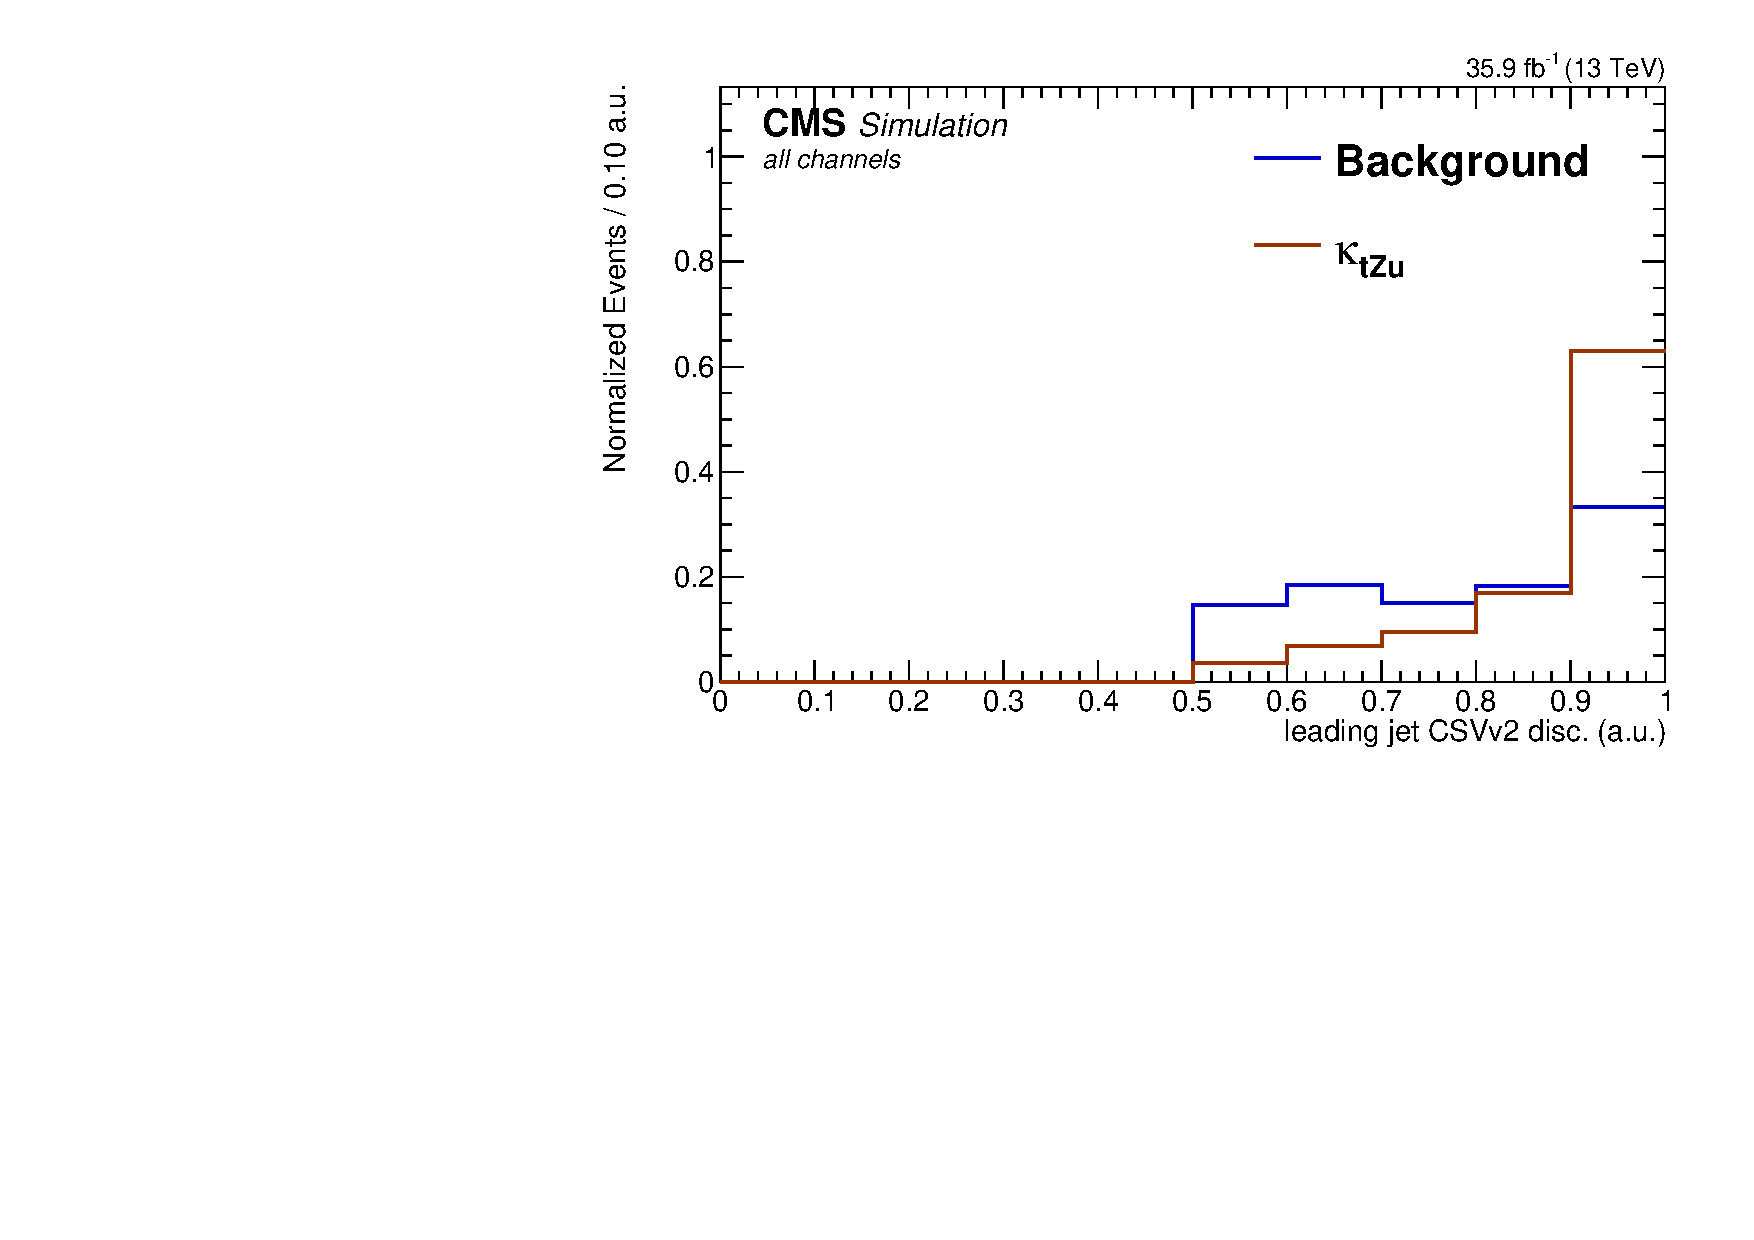
\includegraphics[width=0.3\linewidth]{6_Search/Figures/BDTinputvars/Zut/singletop_MVA_bdiscCSVv2_jet_0_all_Normalized}
    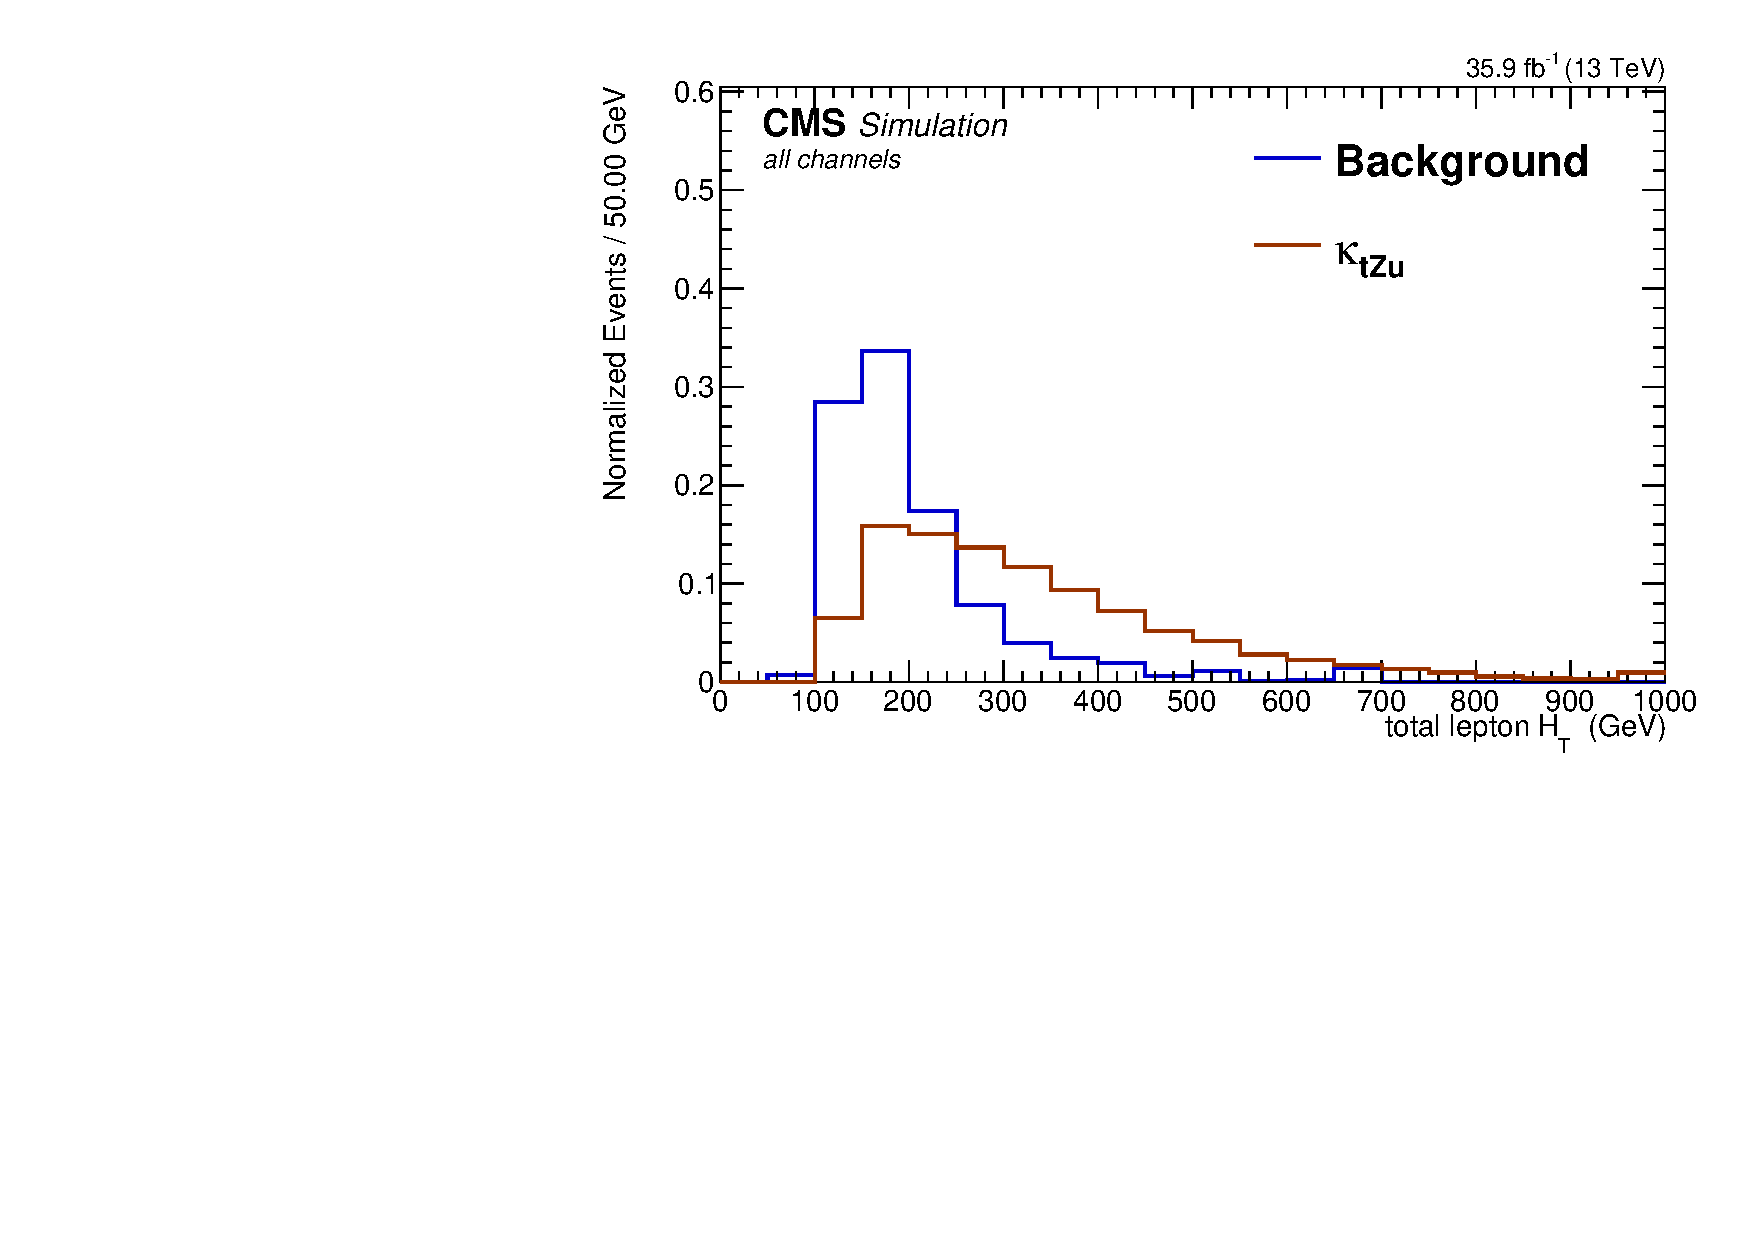
\includegraphics[width=0.3\linewidth]{6_Search/Figures/BDTinputvars/Zut/singletop_MVA_TotalHt_lep_all_Normalized}
    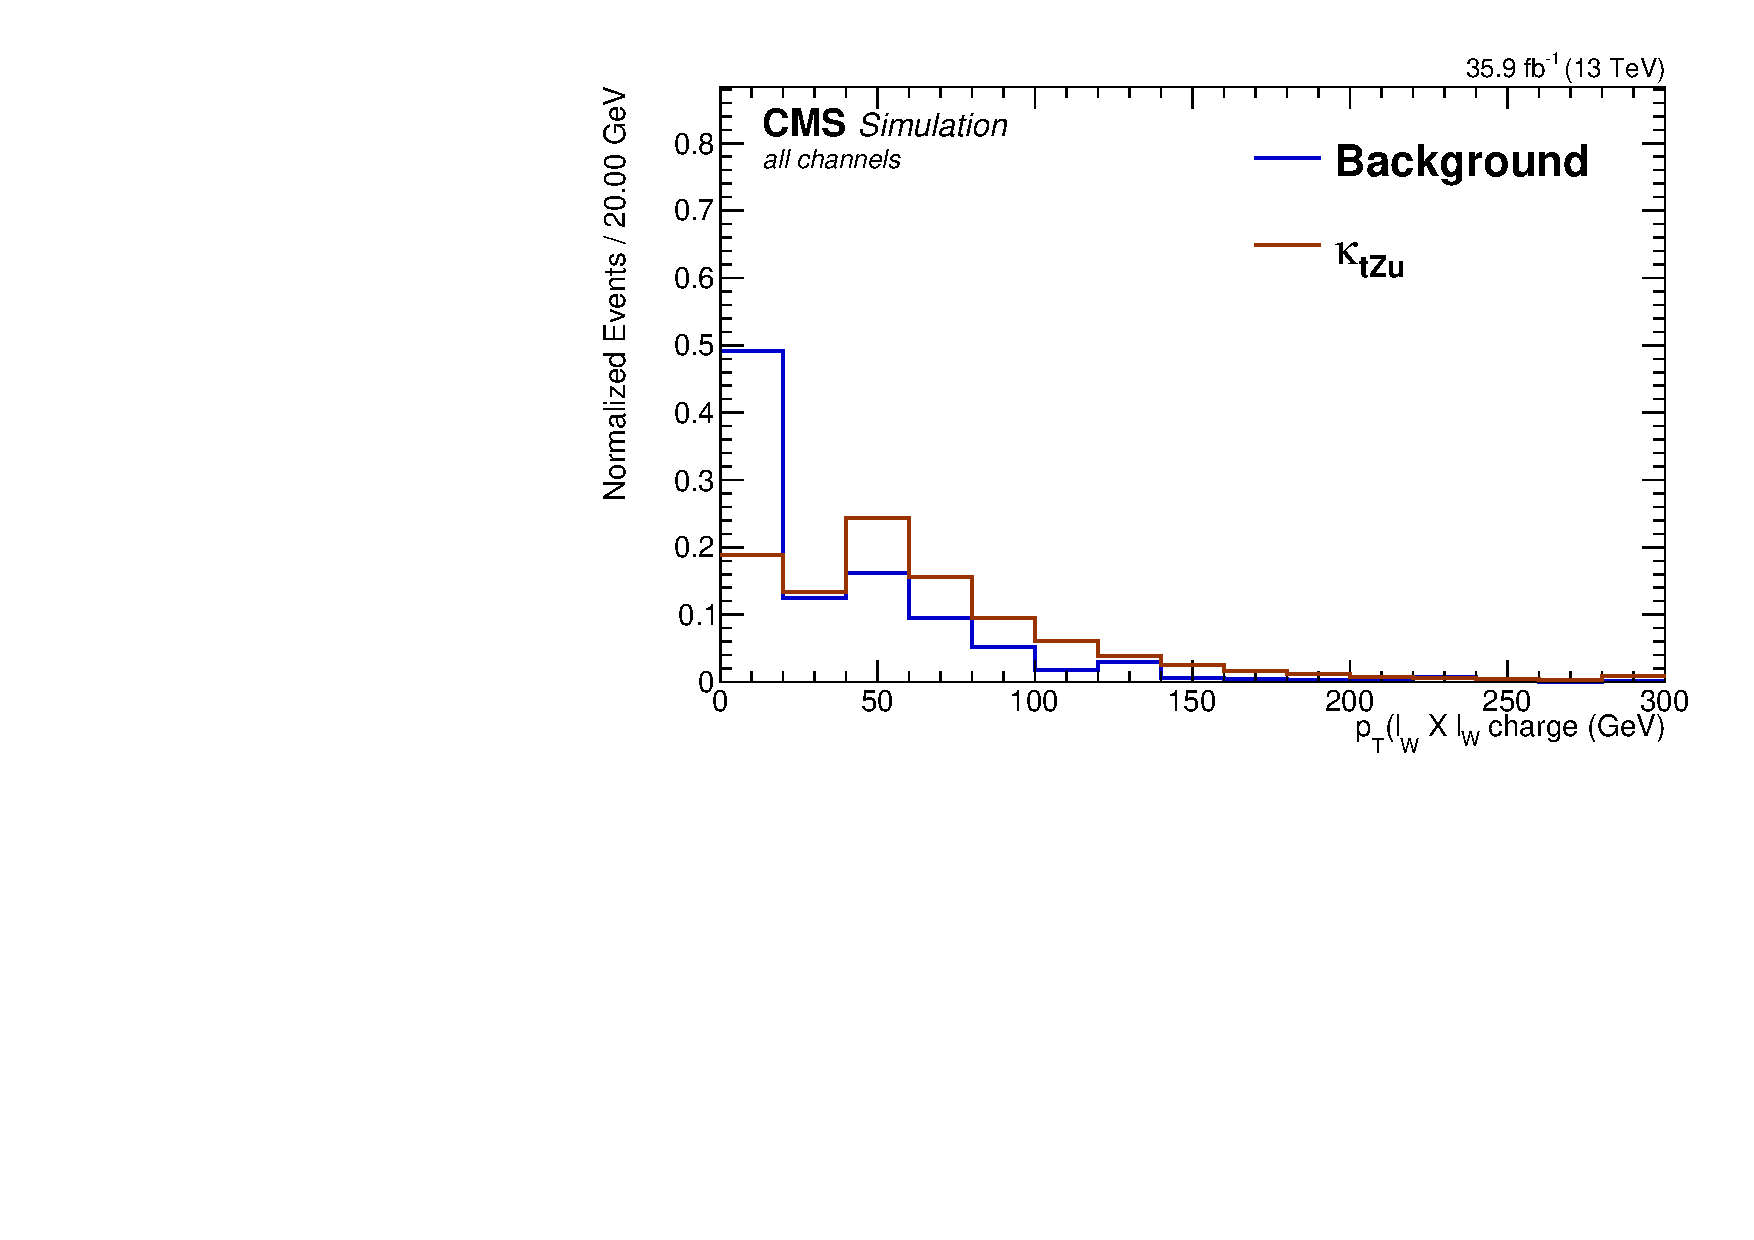
\includegraphics[width=0.3\linewidth]{6_Search/Figures/BDTinputvars/Zut/singletop_MVA_ptWQ_all_Normalized}
 	\caption{The normalised input variables for reconstructing the multivariate discriminator in the \STSR\ for the \Zut\ vertex.}
	\label{fig:singletopZutnormalized}
\end{figure}




\clearpage
\subsection{BDTs}
\label{sec:BDTs}
The normalised distributions of the multivariate discriminator, including the \NPL\ background are shown in this section. \todo{Beschrijf plotjes}
\begin{figure}[htbp]
	\centering
	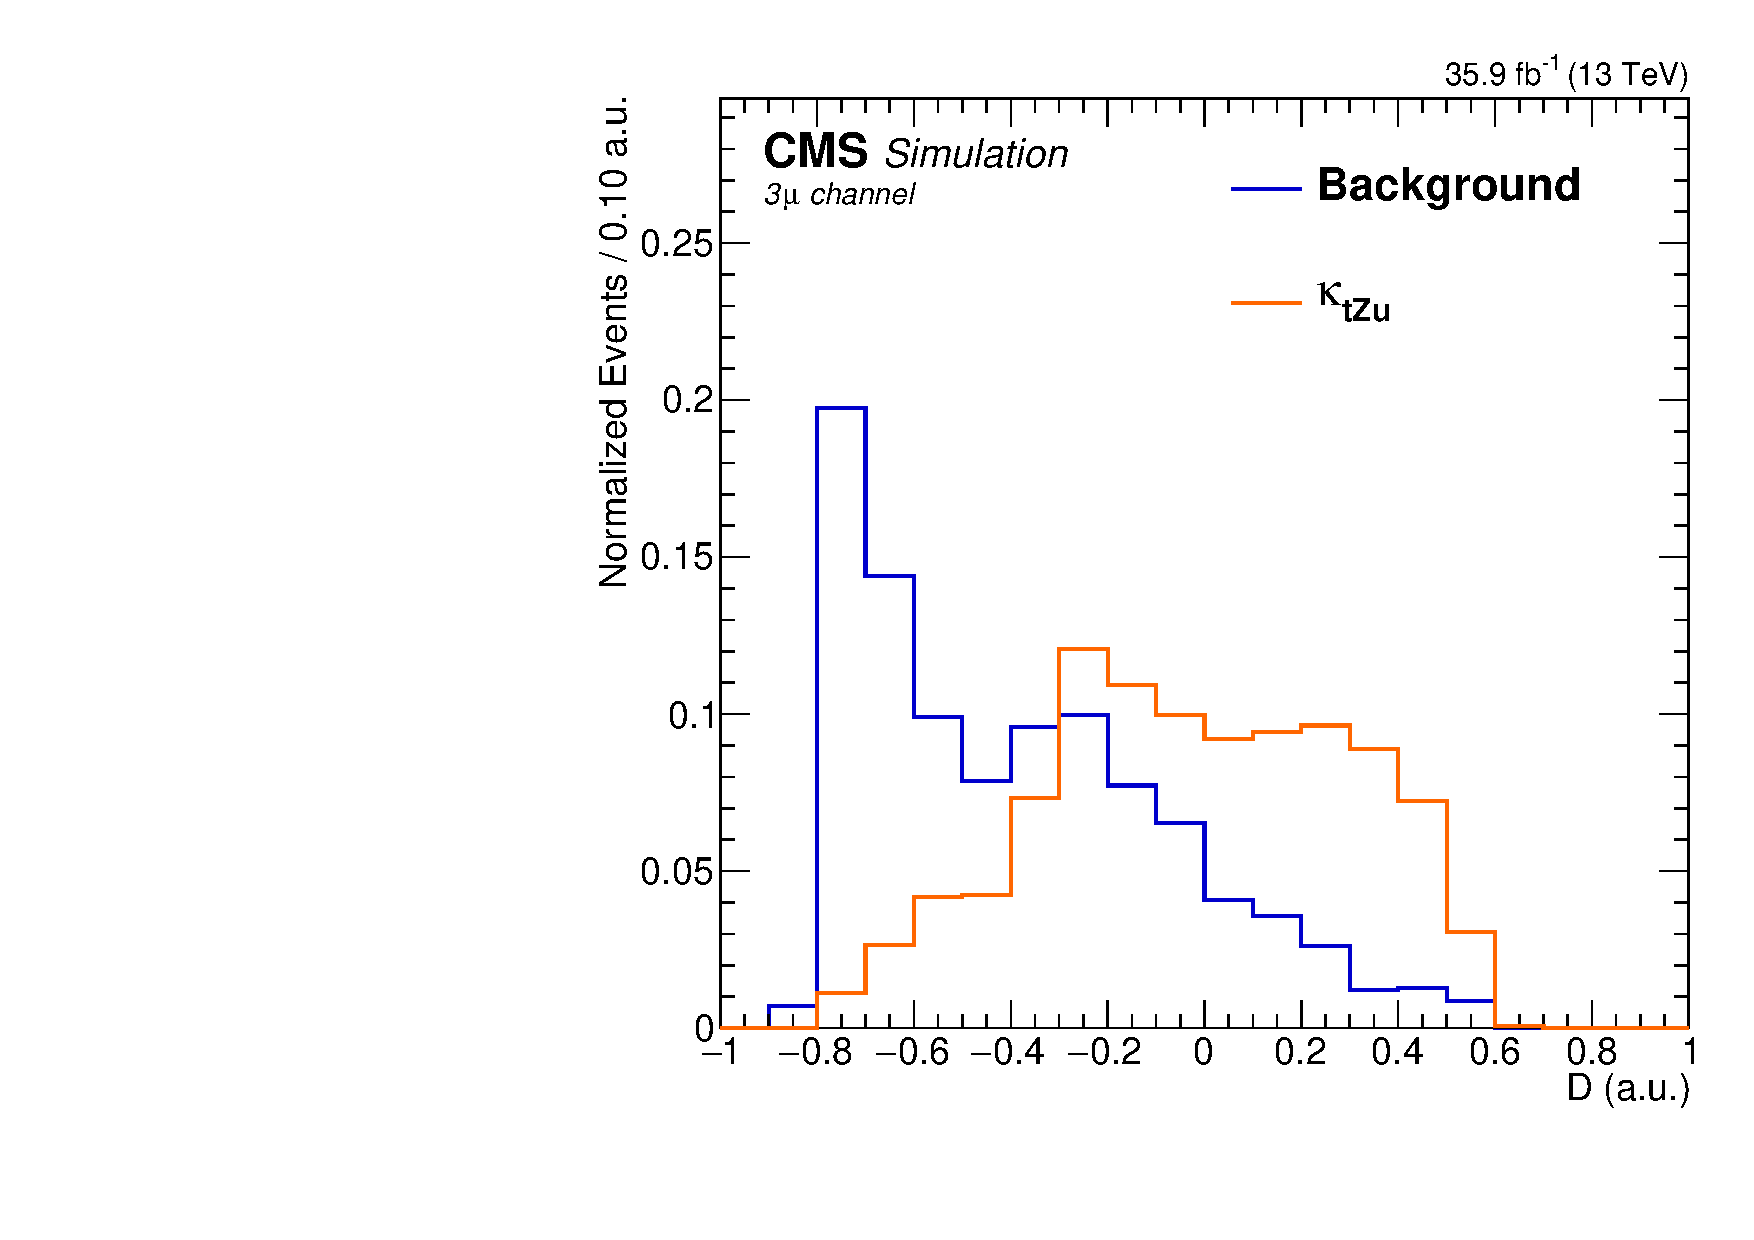
\includegraphics[width=0.49\linewidth]{6_Search/Figures/BDTdistributionsNorm/toppair_Zut_BDT_uuu_Normalized}
	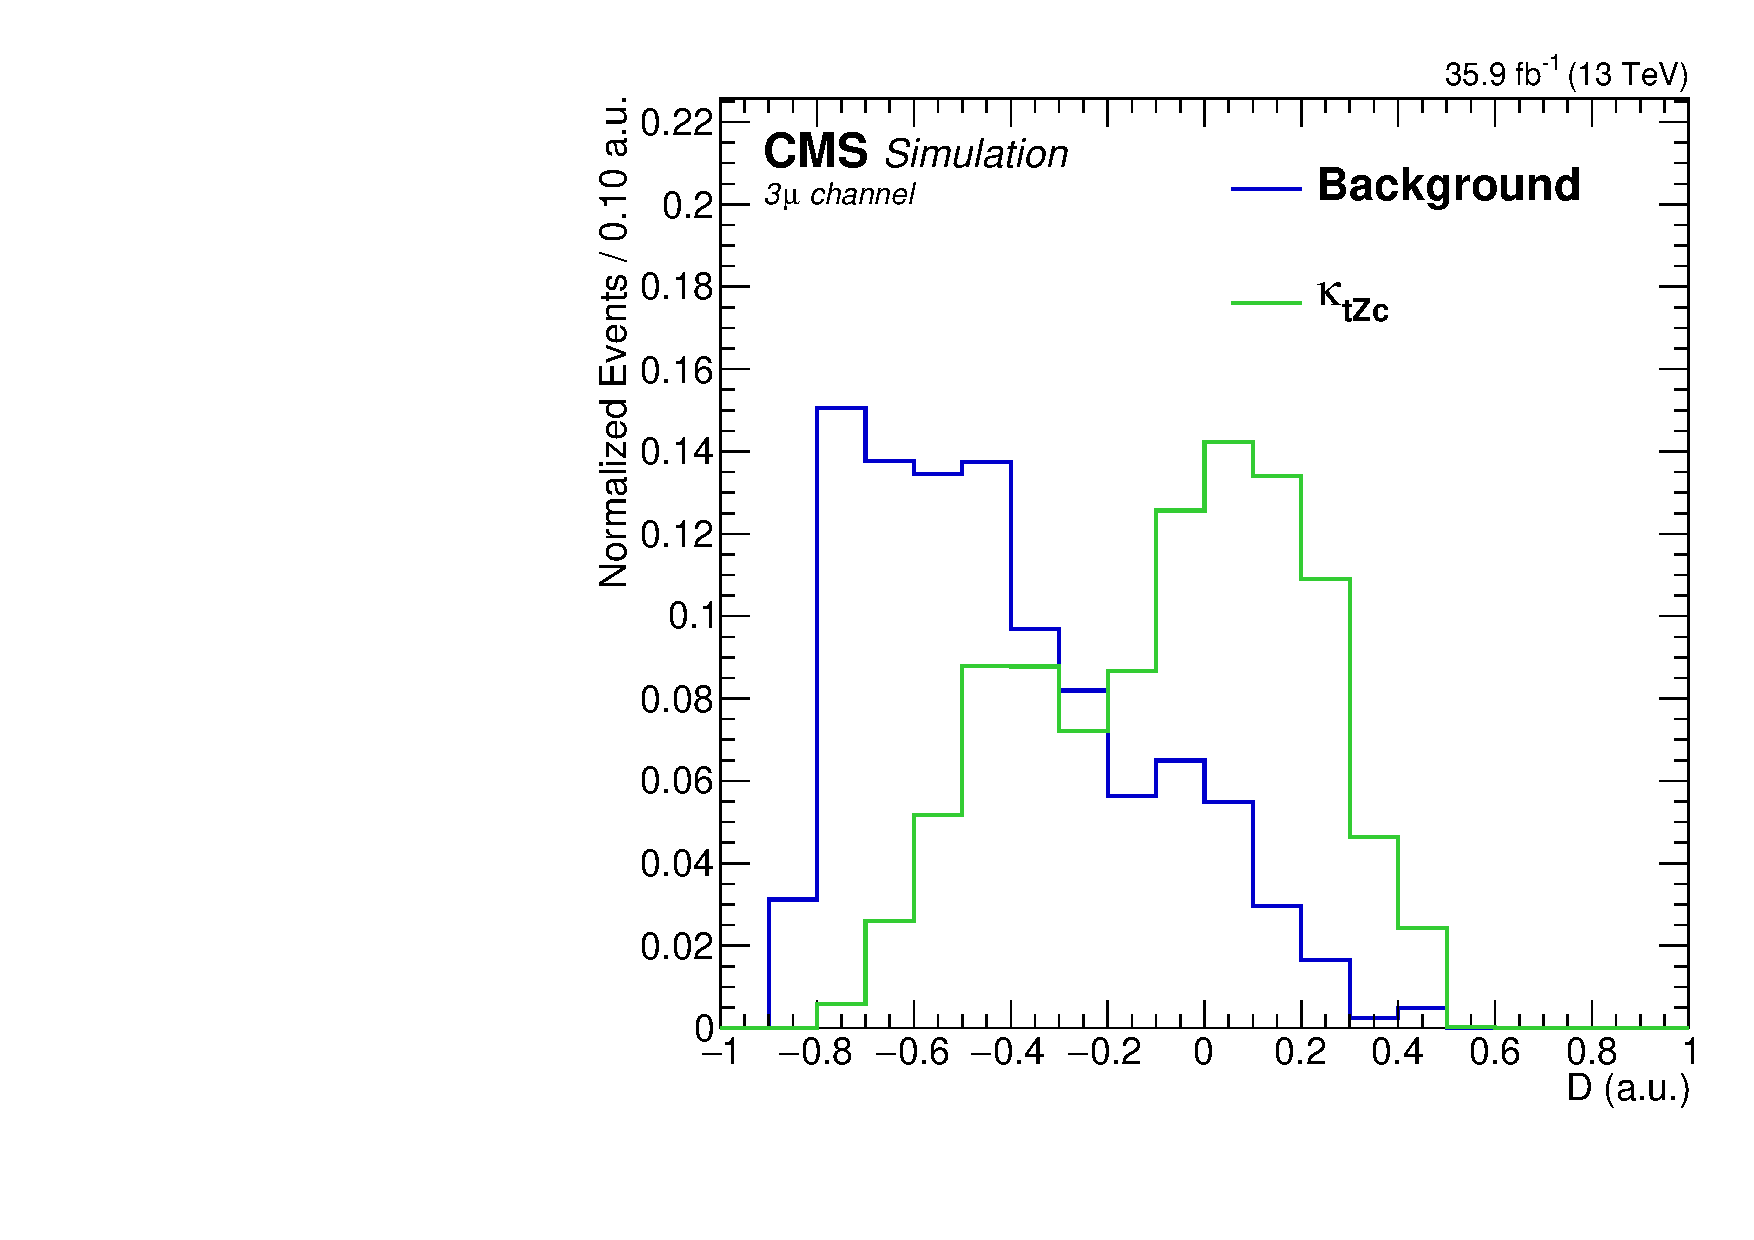
\includegraphics[width=0.49\linewidth]{6_Search/Figures/BDTdistributionsNorm/toppair_Zct_BDT_uuu_Normalized}
	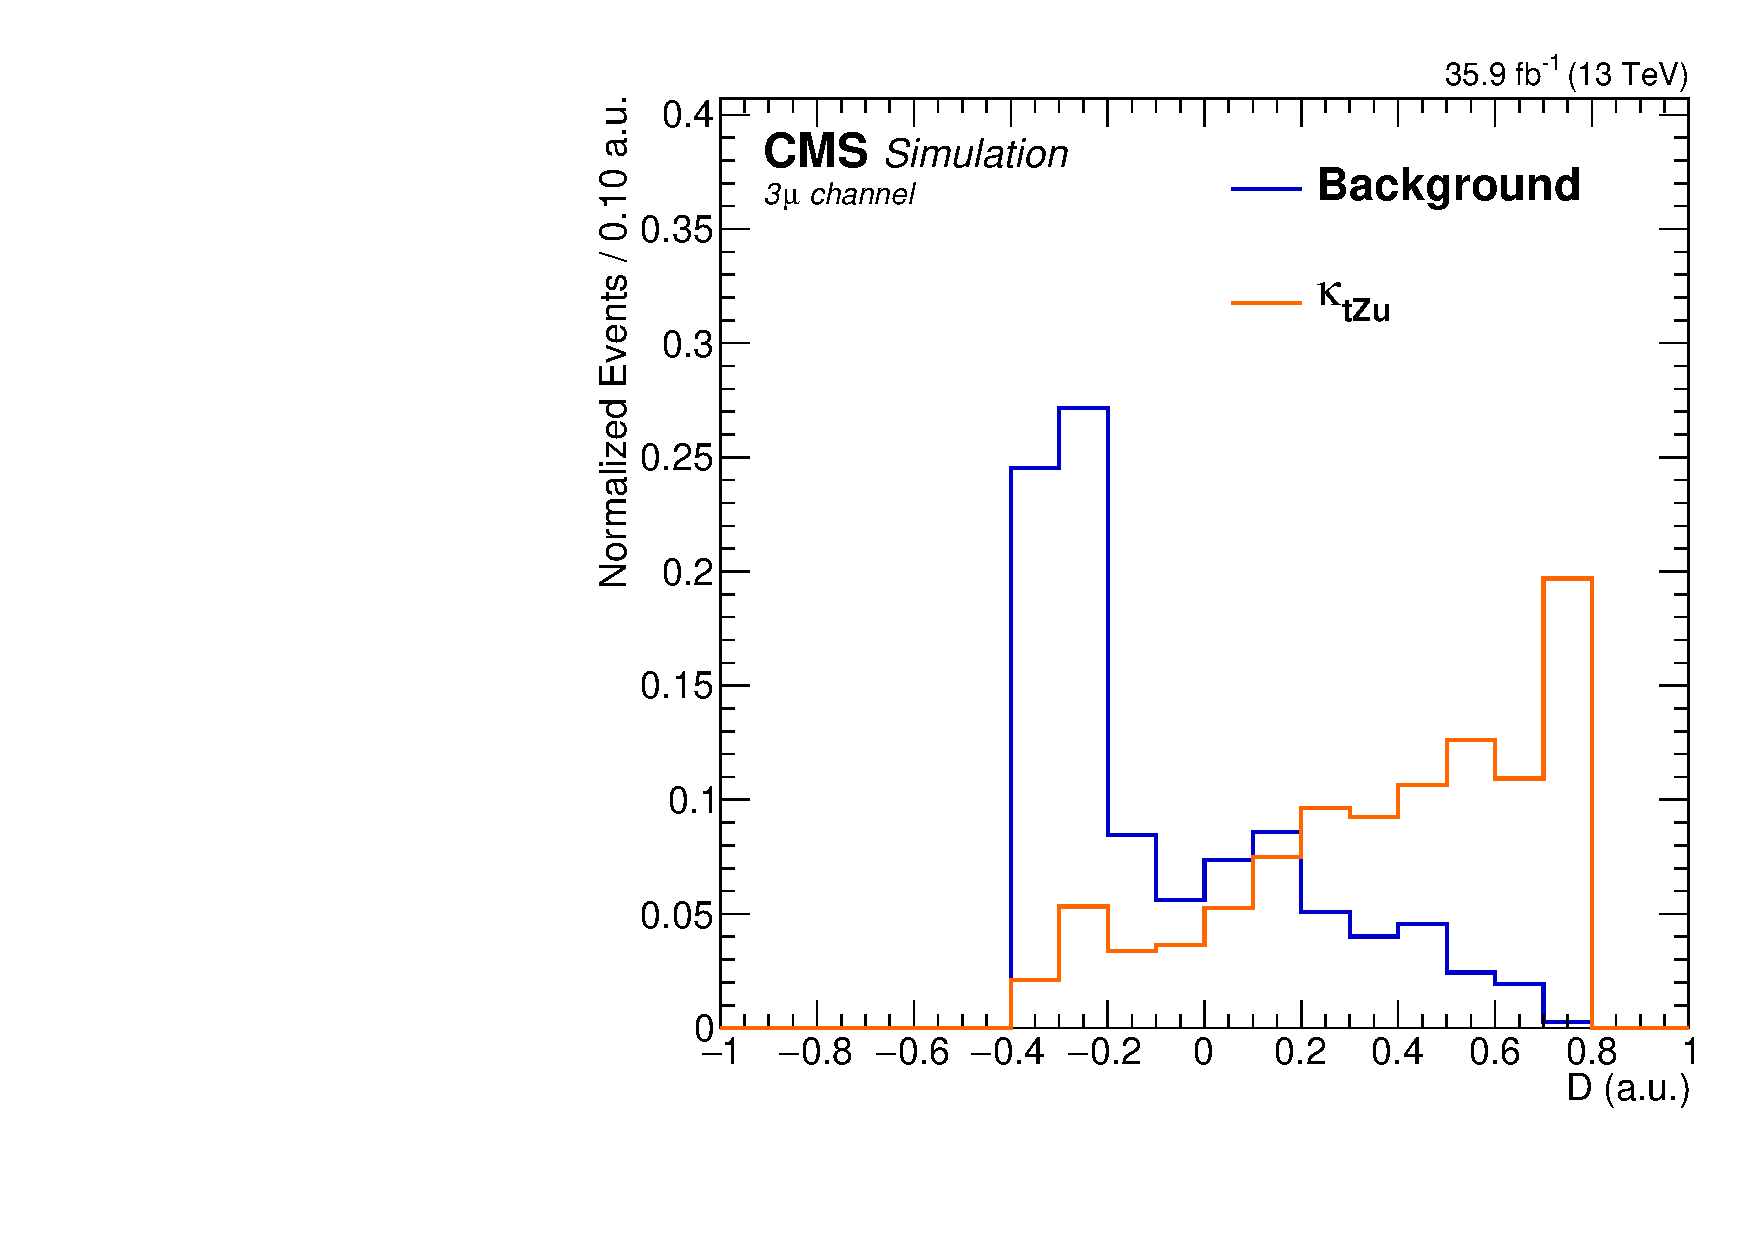
\includegraphics[width=0.49\linewidth]{6_Search/Figures/BDTdistributionsNorm/singletop_Zut_BDT_uuu_Normalized}
	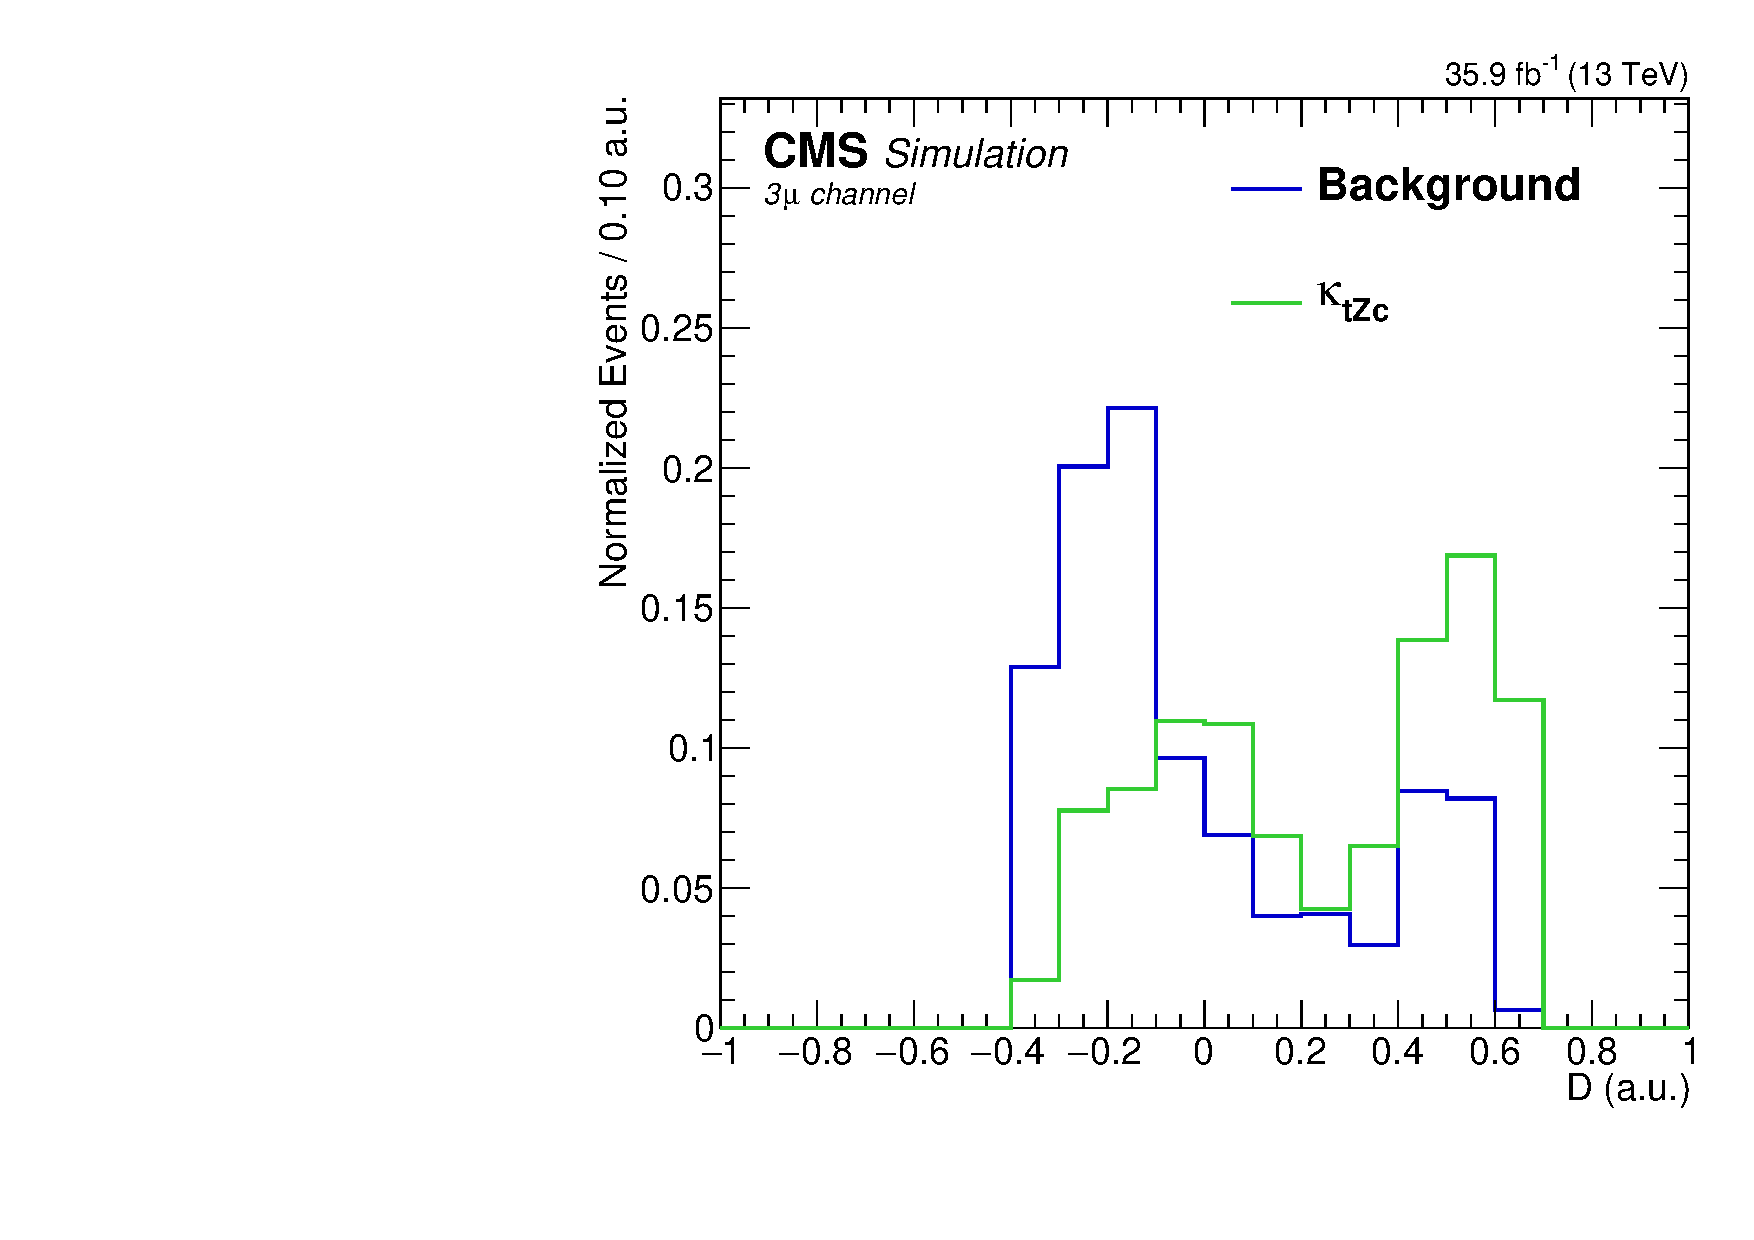
\includegraphics[width=0.49\linewidth]{6_Search/Figures/BDTdistributionsNorm/singletop_Zct_BDT_uuu_Normalized}
	\caption{Normalised distributions of the discriminating variable before the fit, \mumumu\ lepton channel. Upper left: \TTSR\ \Zut , upper right: \TTSR\ \Zct ; lower left: \STSR\  \Zut , lower right: \STSR\  \Zct .}
	\label{fig:bdtuuunorm}
\end{figure}	


\begin{figure}[htbp]
	\centering
	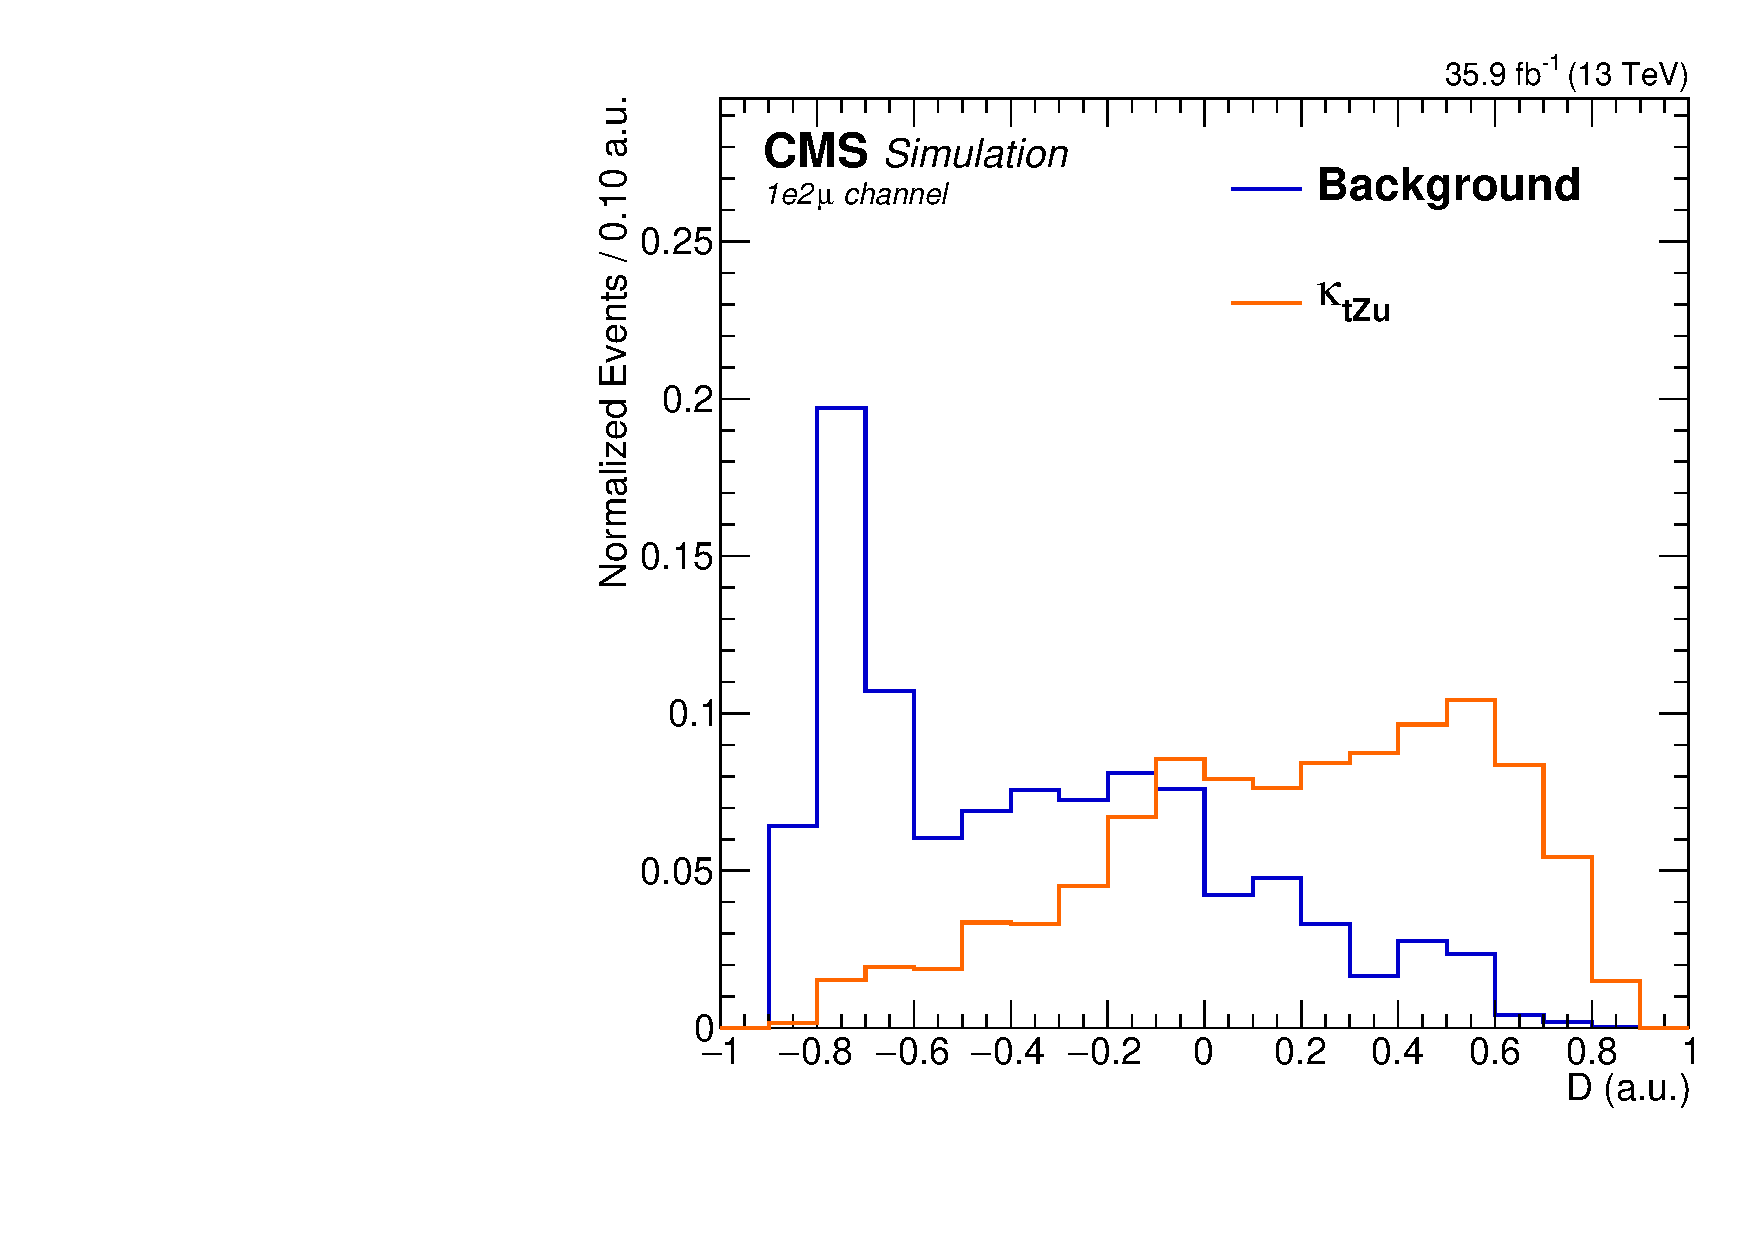
\includegraphics[width=0.49\linewidth]{6_Search/Figures/BDTdistributionsNorm/toppair_Zut_BDT_uue_Normalized}
	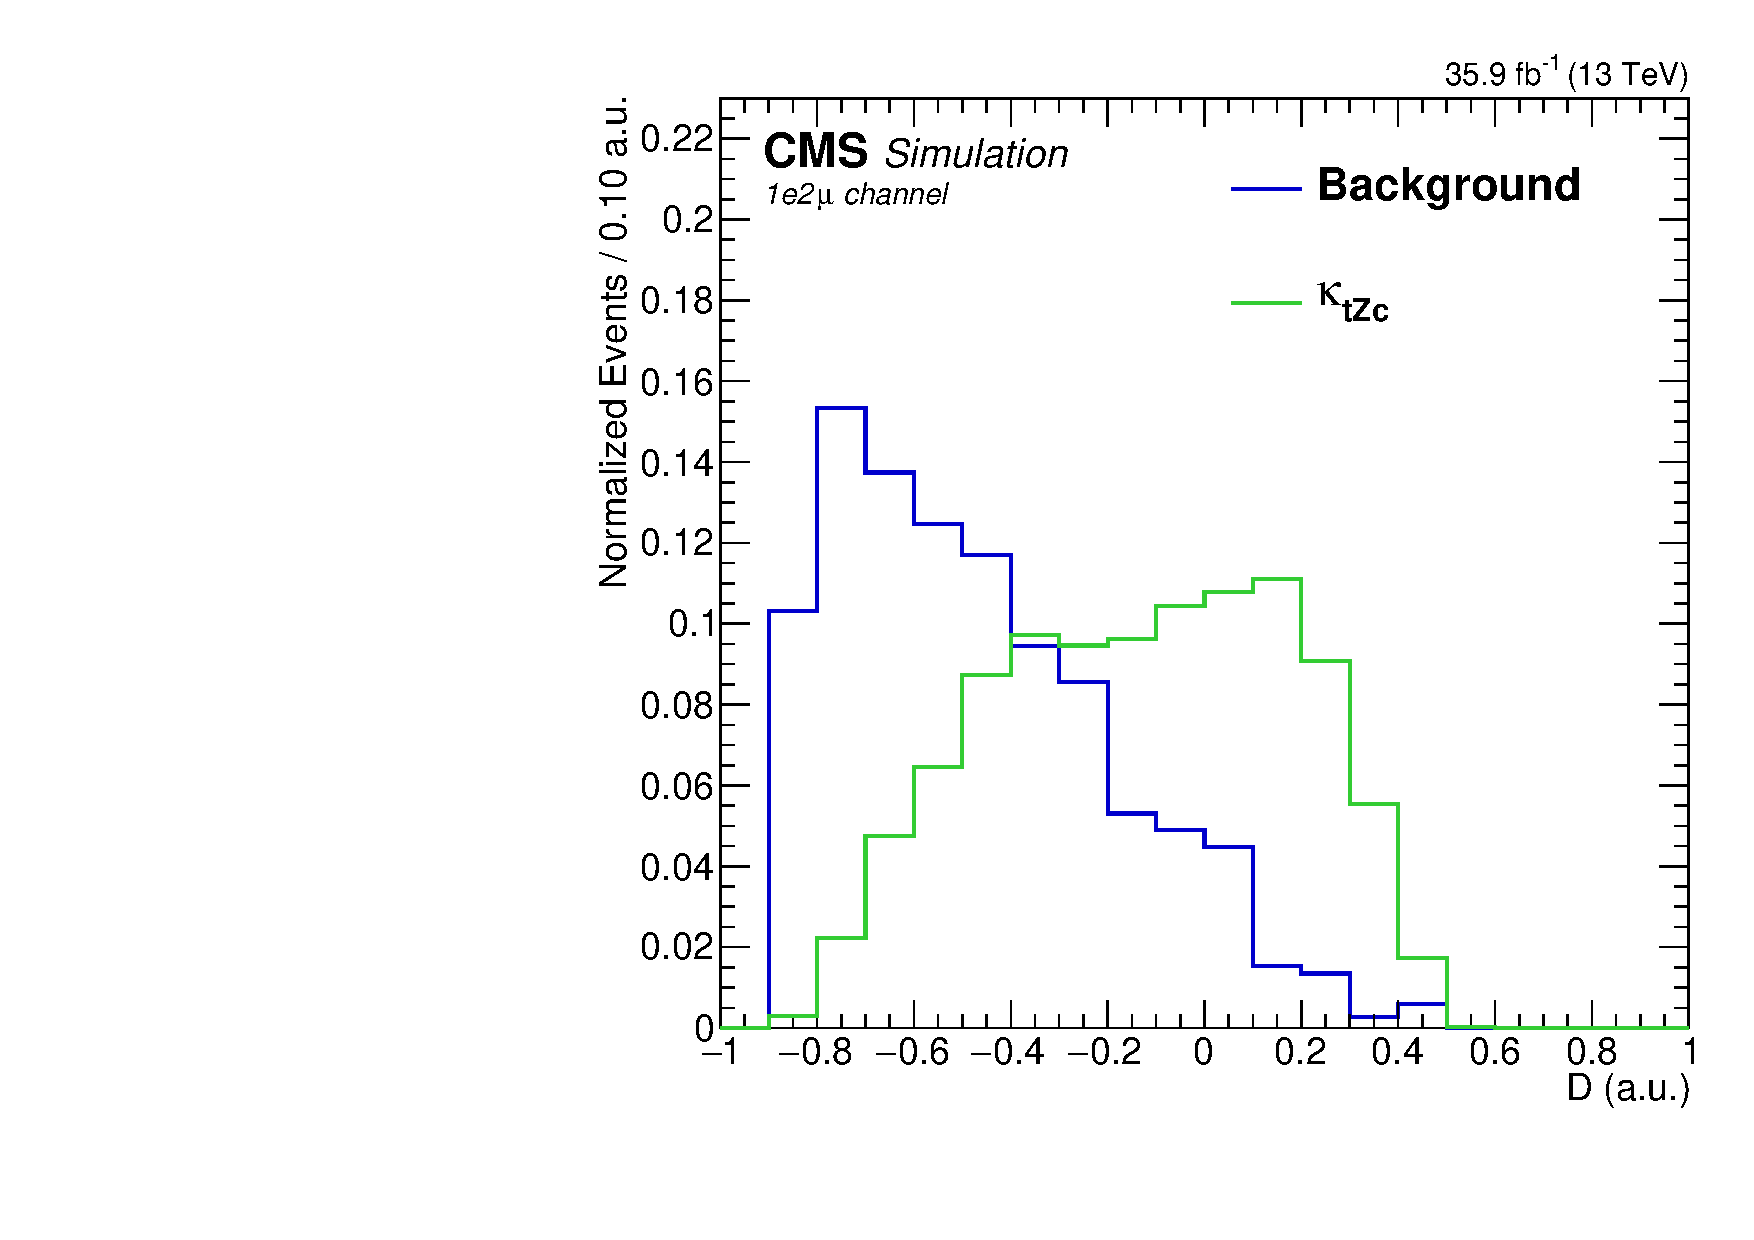
\includegraphics[width=0.49\linewidth]{6_Search/Figures/BDTdistributionsNorm/toppair_Zct_BDT_uue_Normalized}
	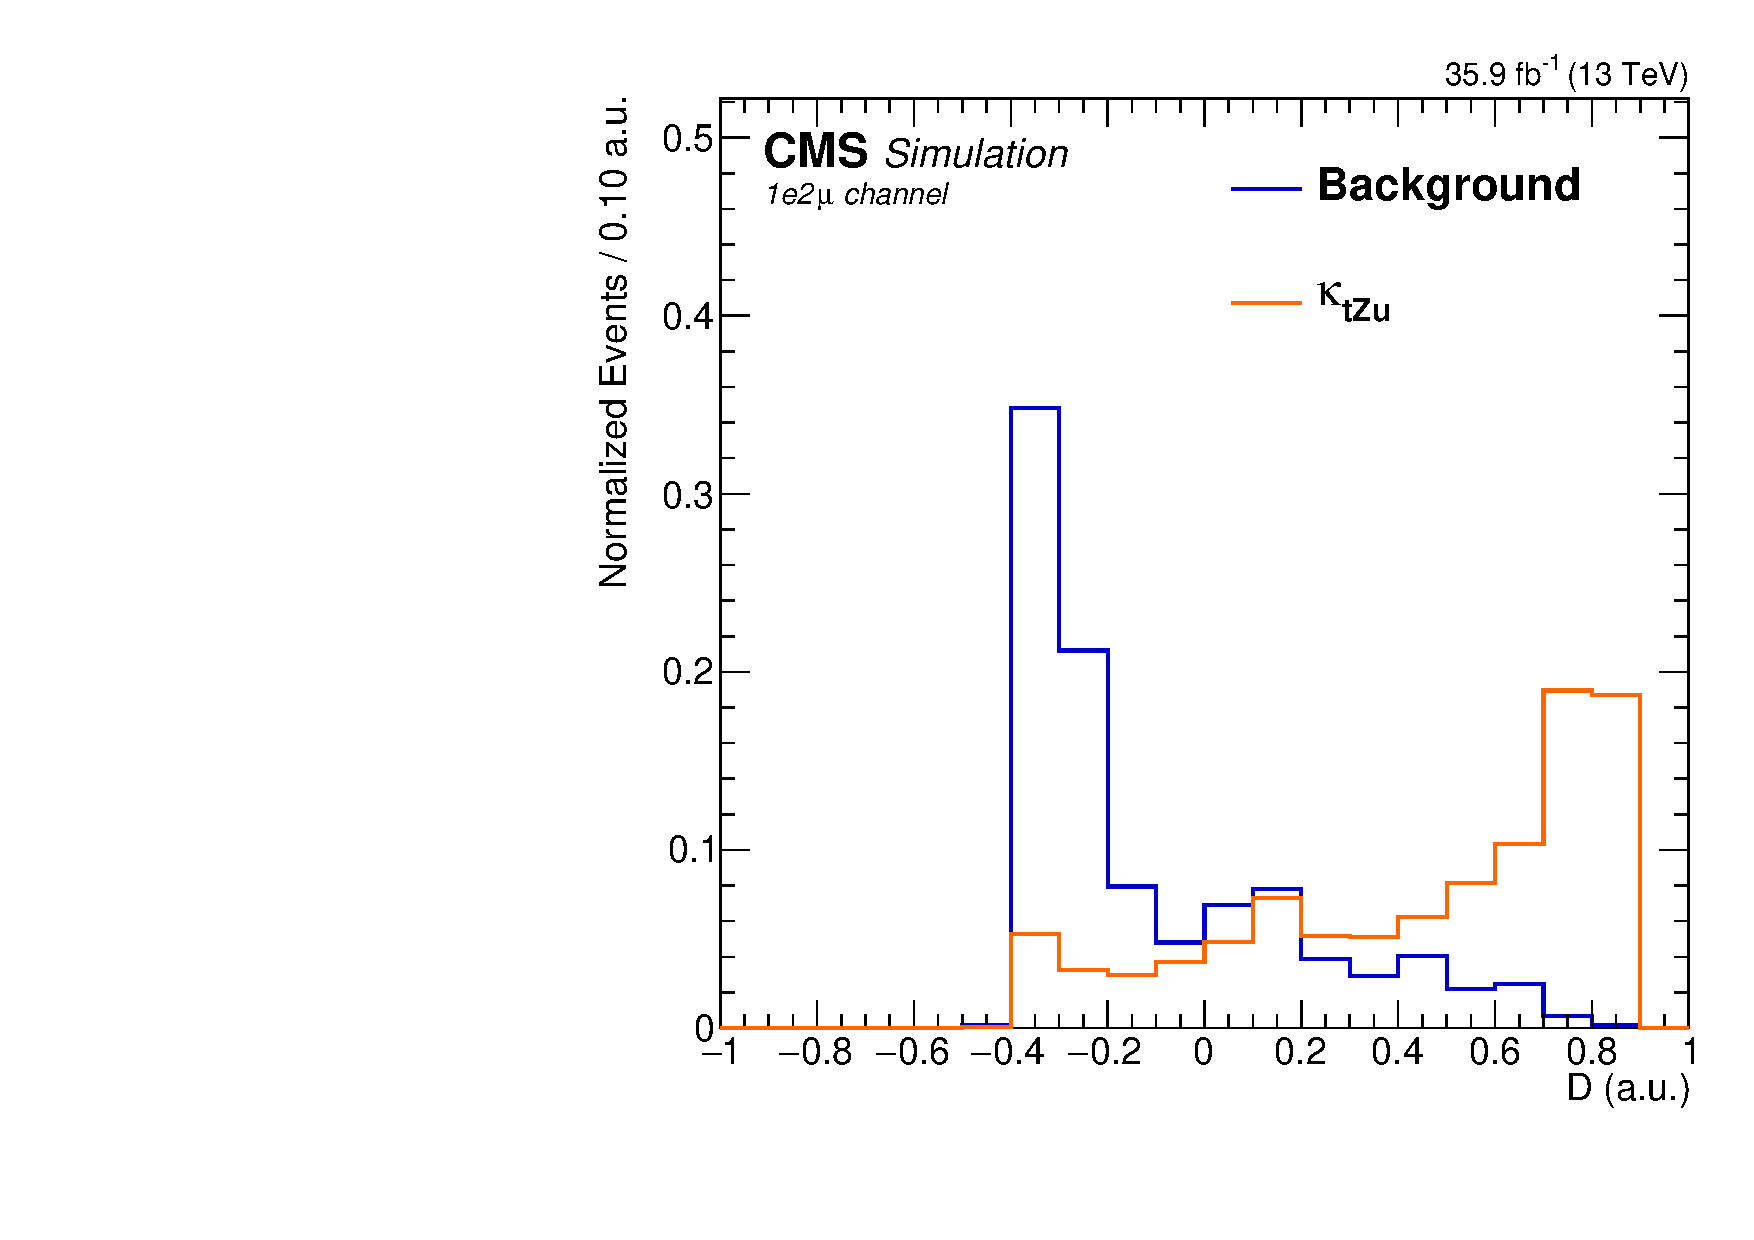
\includegraphics[width=0.49\linewidth]{6_Search/Figures/BDTdistributionsNorm/singletop_Zut_BDT_uue_Normalized}
	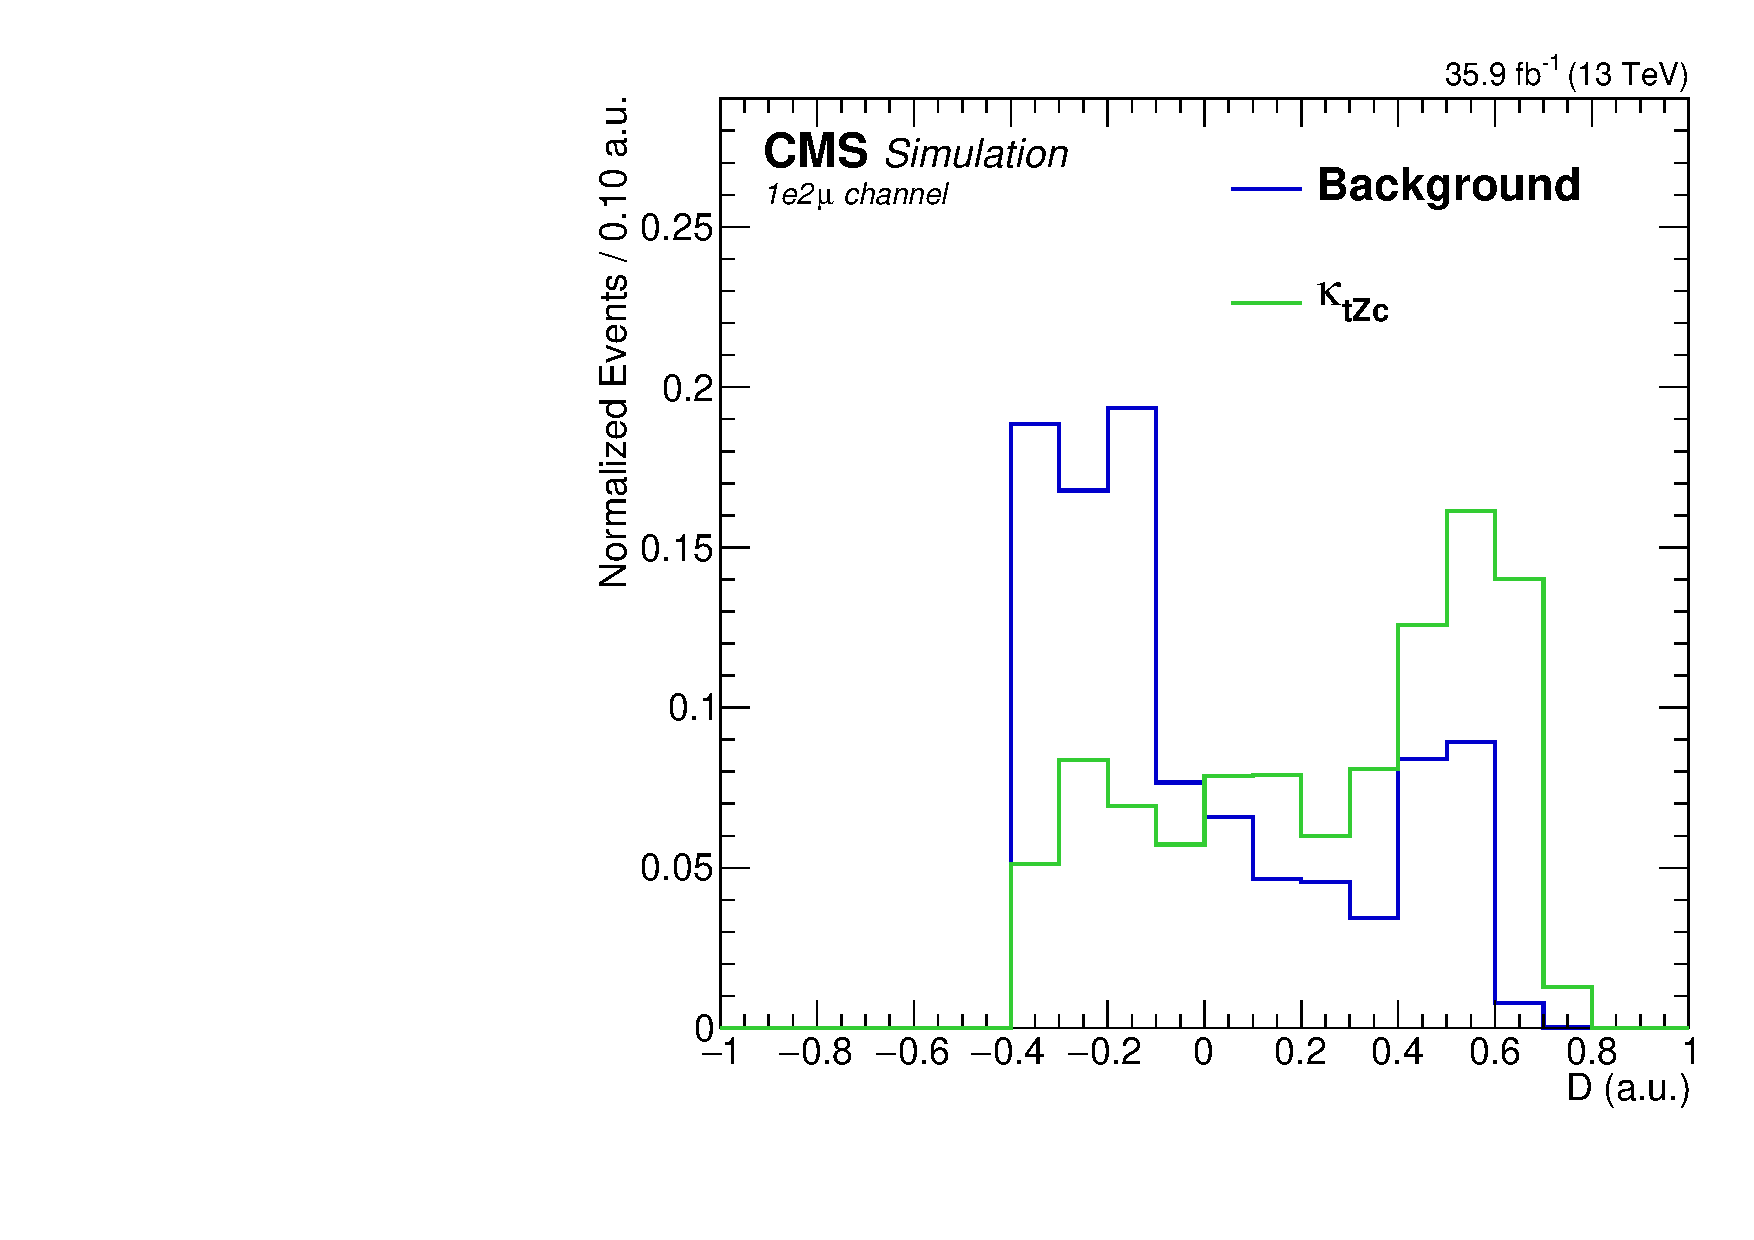
\includegraphics[width=0.49\linewidth]{6_Search/Figures/BDTdistributionsNorm/singletop_Zct_BDT_uue_Normalized}
	\caption{Normalised distributions of the discriminating variable before the fit, \emumu\ lepton channels. Upper left: \TTSR\ \Zut , upper right: \TTSR\ \Zct ; lower left: \STSR\  \Zut , lower right: \STSR\  \Zct .}
	\label{fig:bdtuuenorm}
\end{figure}	

\begin{figure}[htbp]
	\centering
	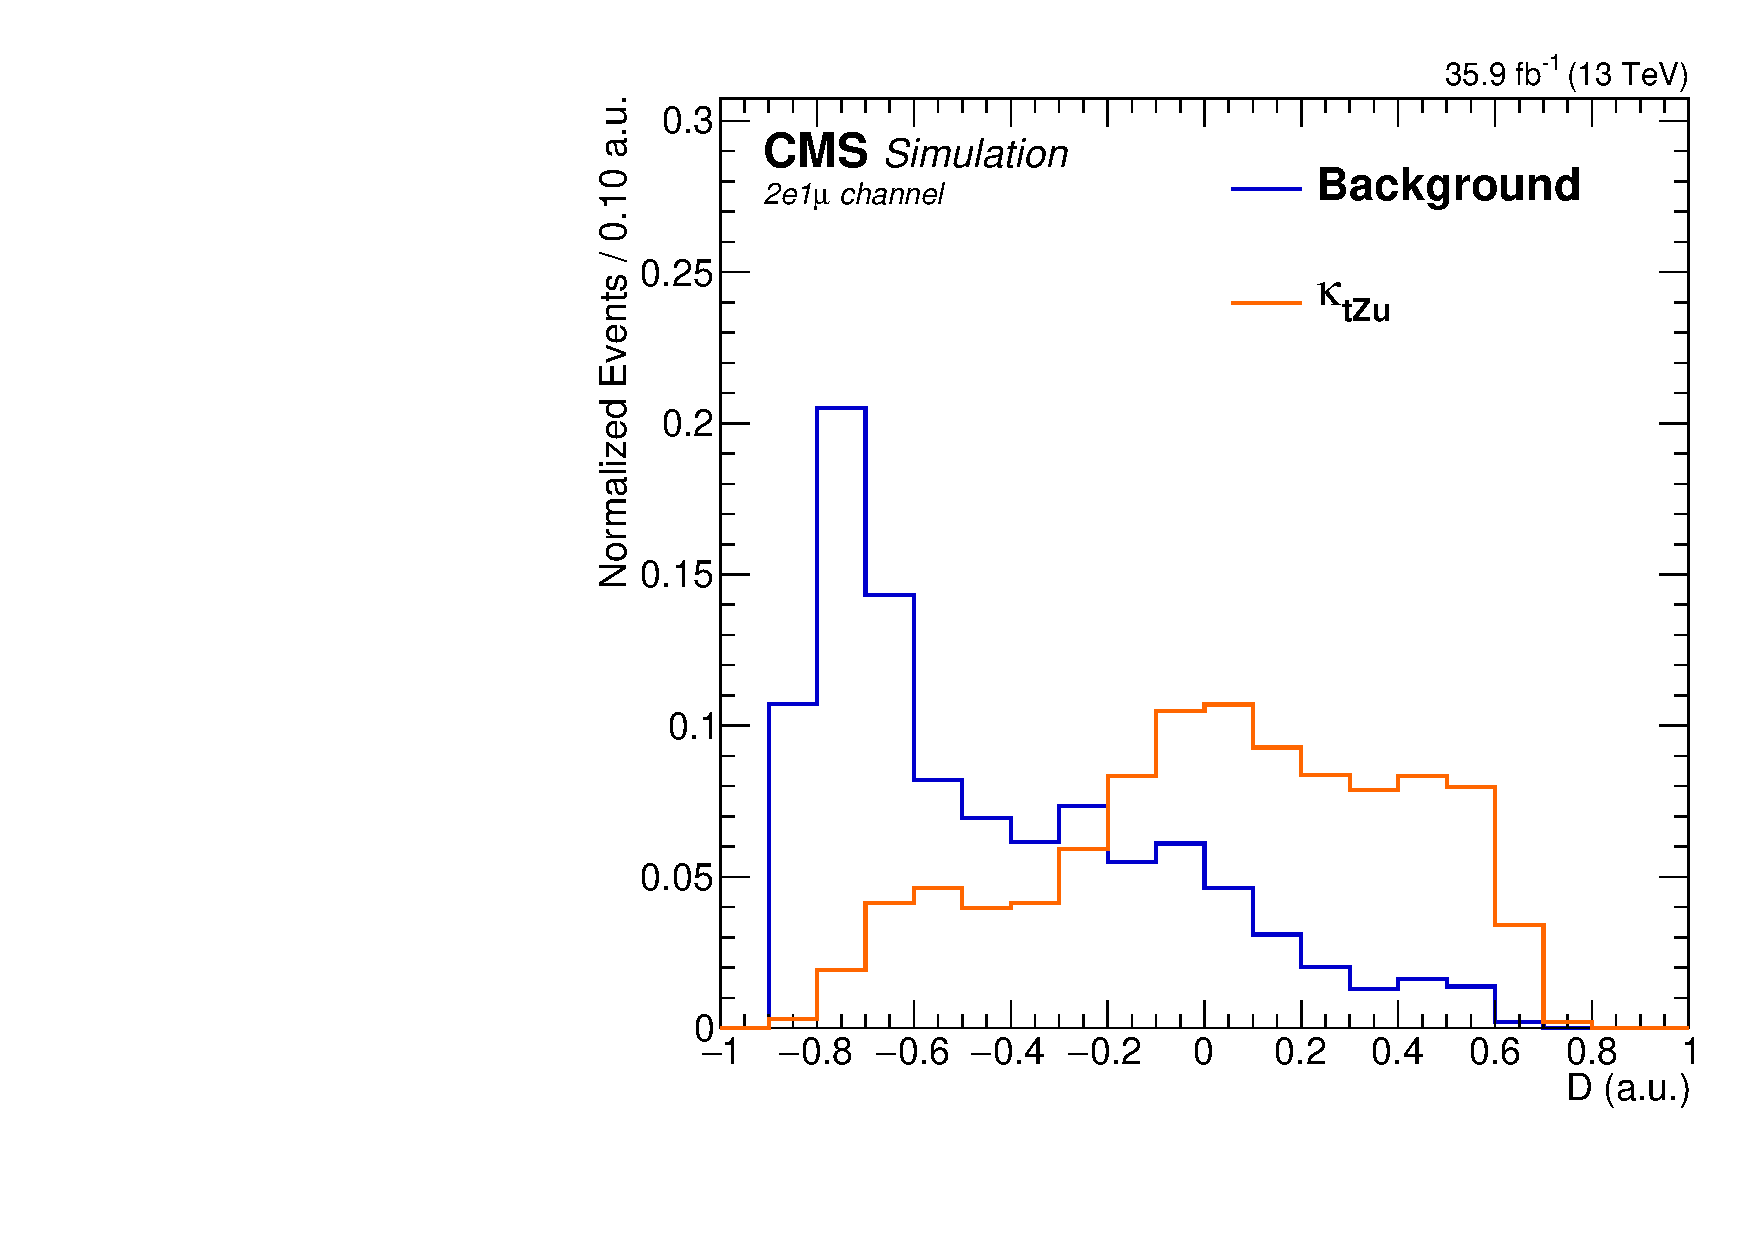
\includegraphics[width=0.49\linewidth]{6_Search/Figures/BDTdistributionsNorm/toppair_Zut_BDT_eeu_Normalized}
	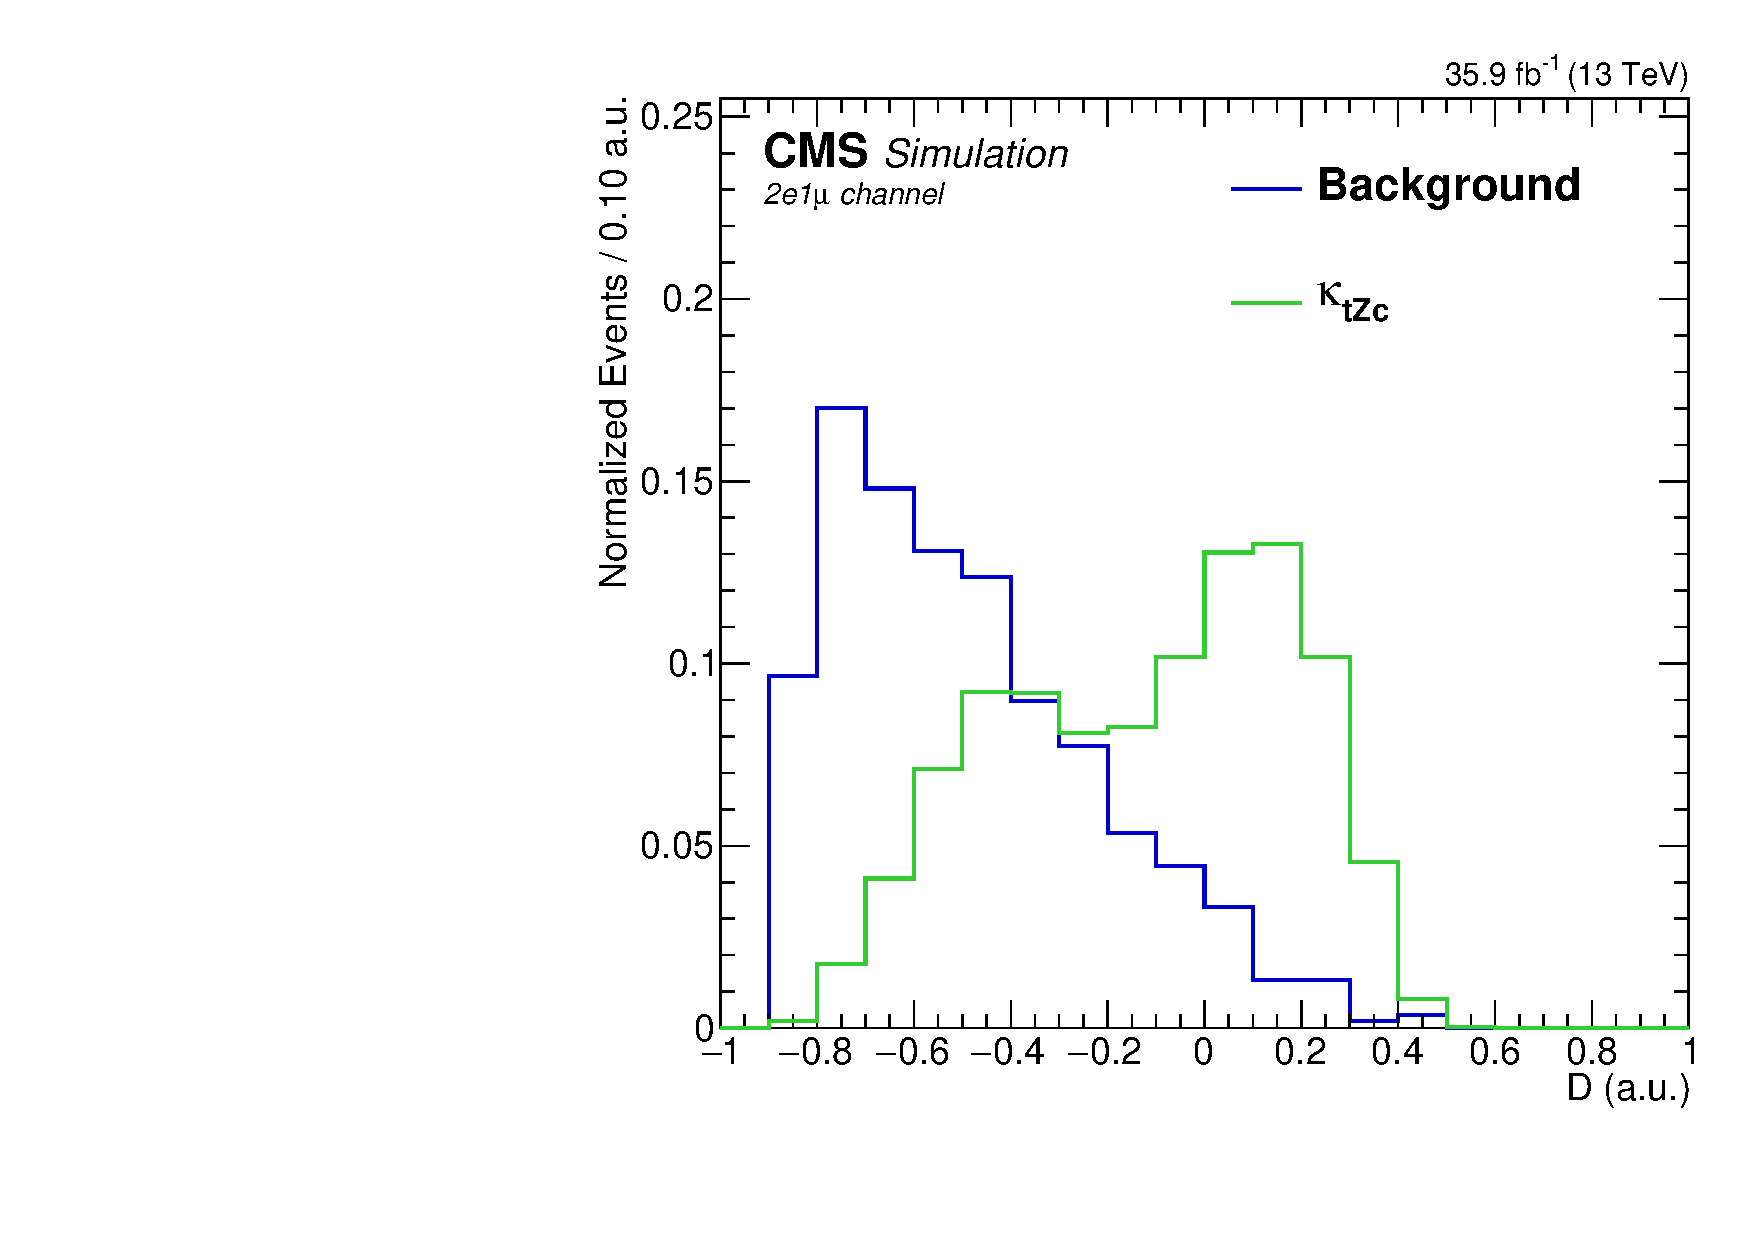
\includegraphics[width=0.49\linewidth]{6_Search/Figures/BDTdistributionsNorm/toppair_Zct_BDT_eeu_Normalized}
	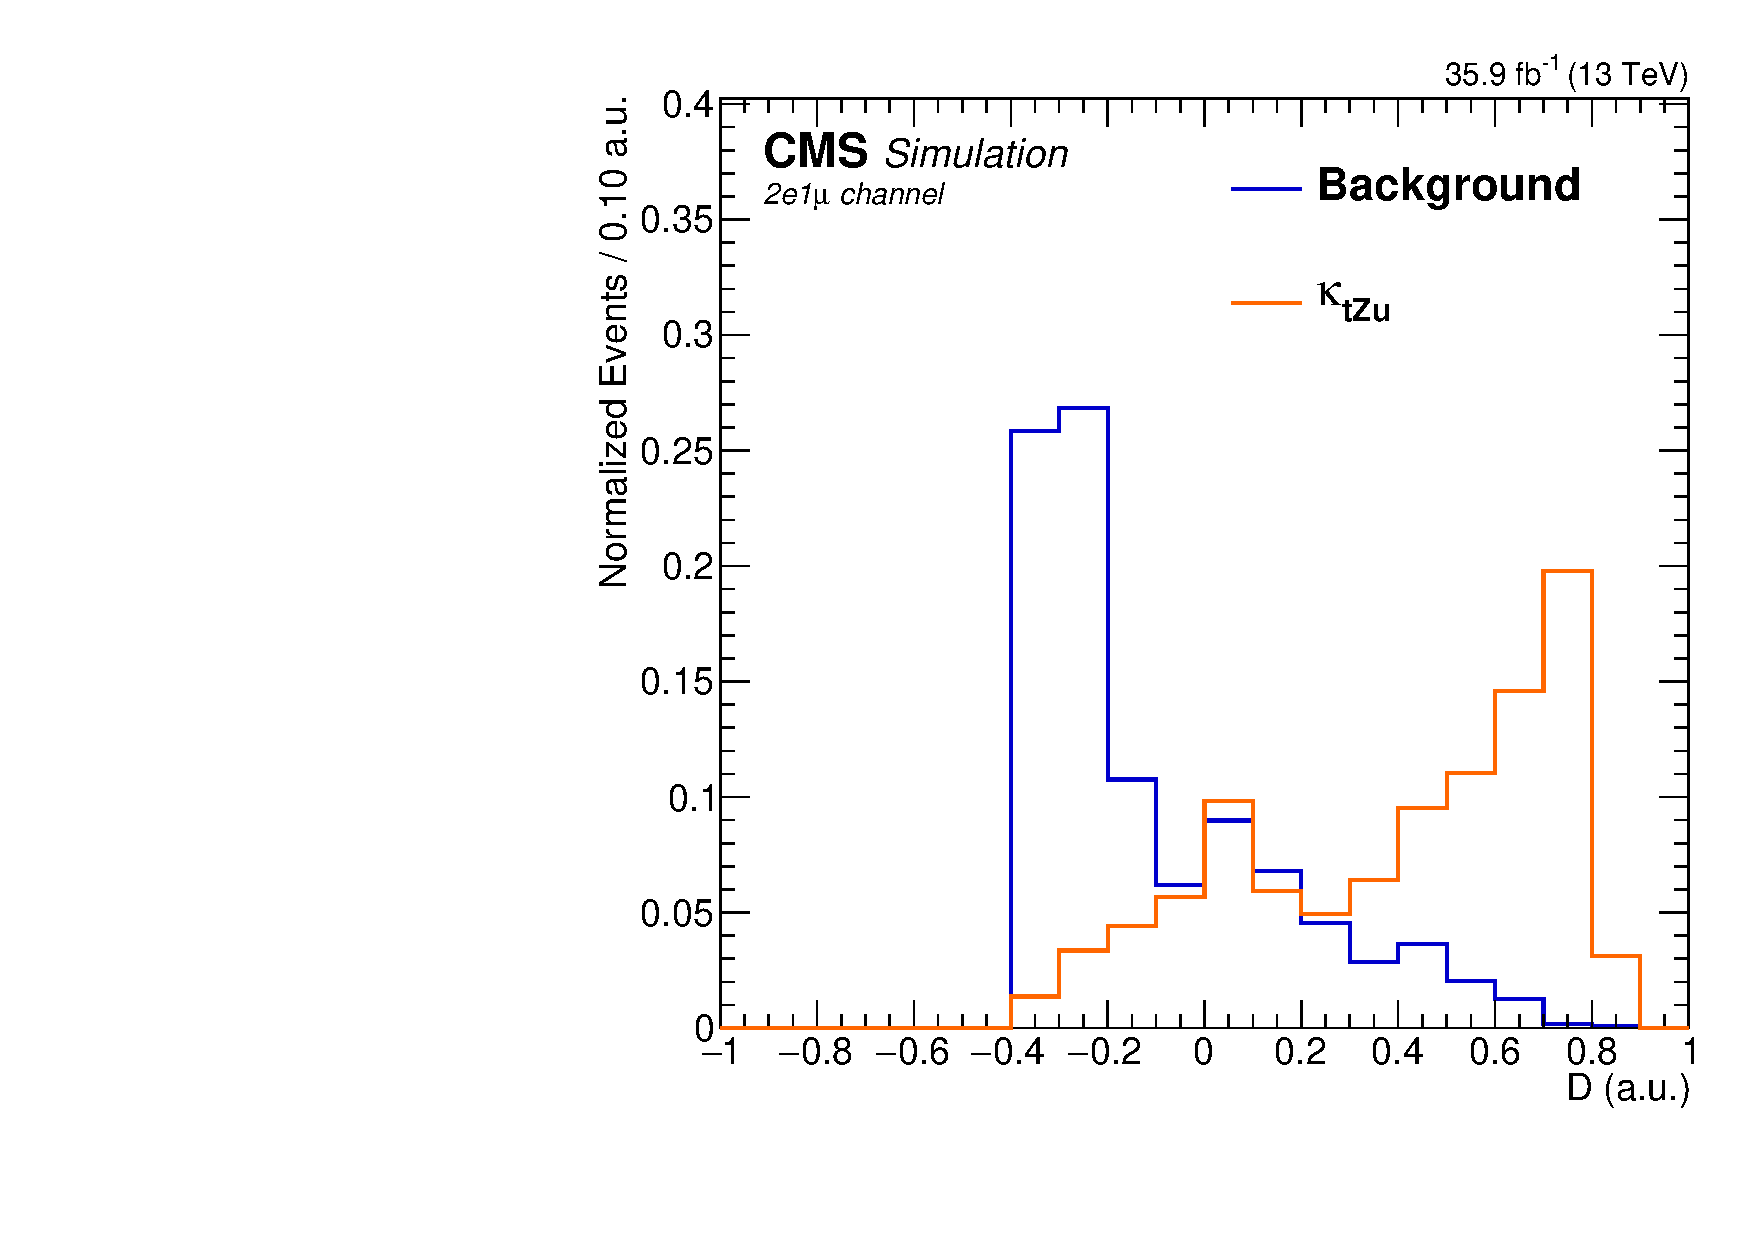
\includegraphics[width=0.49\linewidth]{6_Search/Figures/BDTdistributionsNorm/singletop_Zut_BDT_eeu_Normalized}
	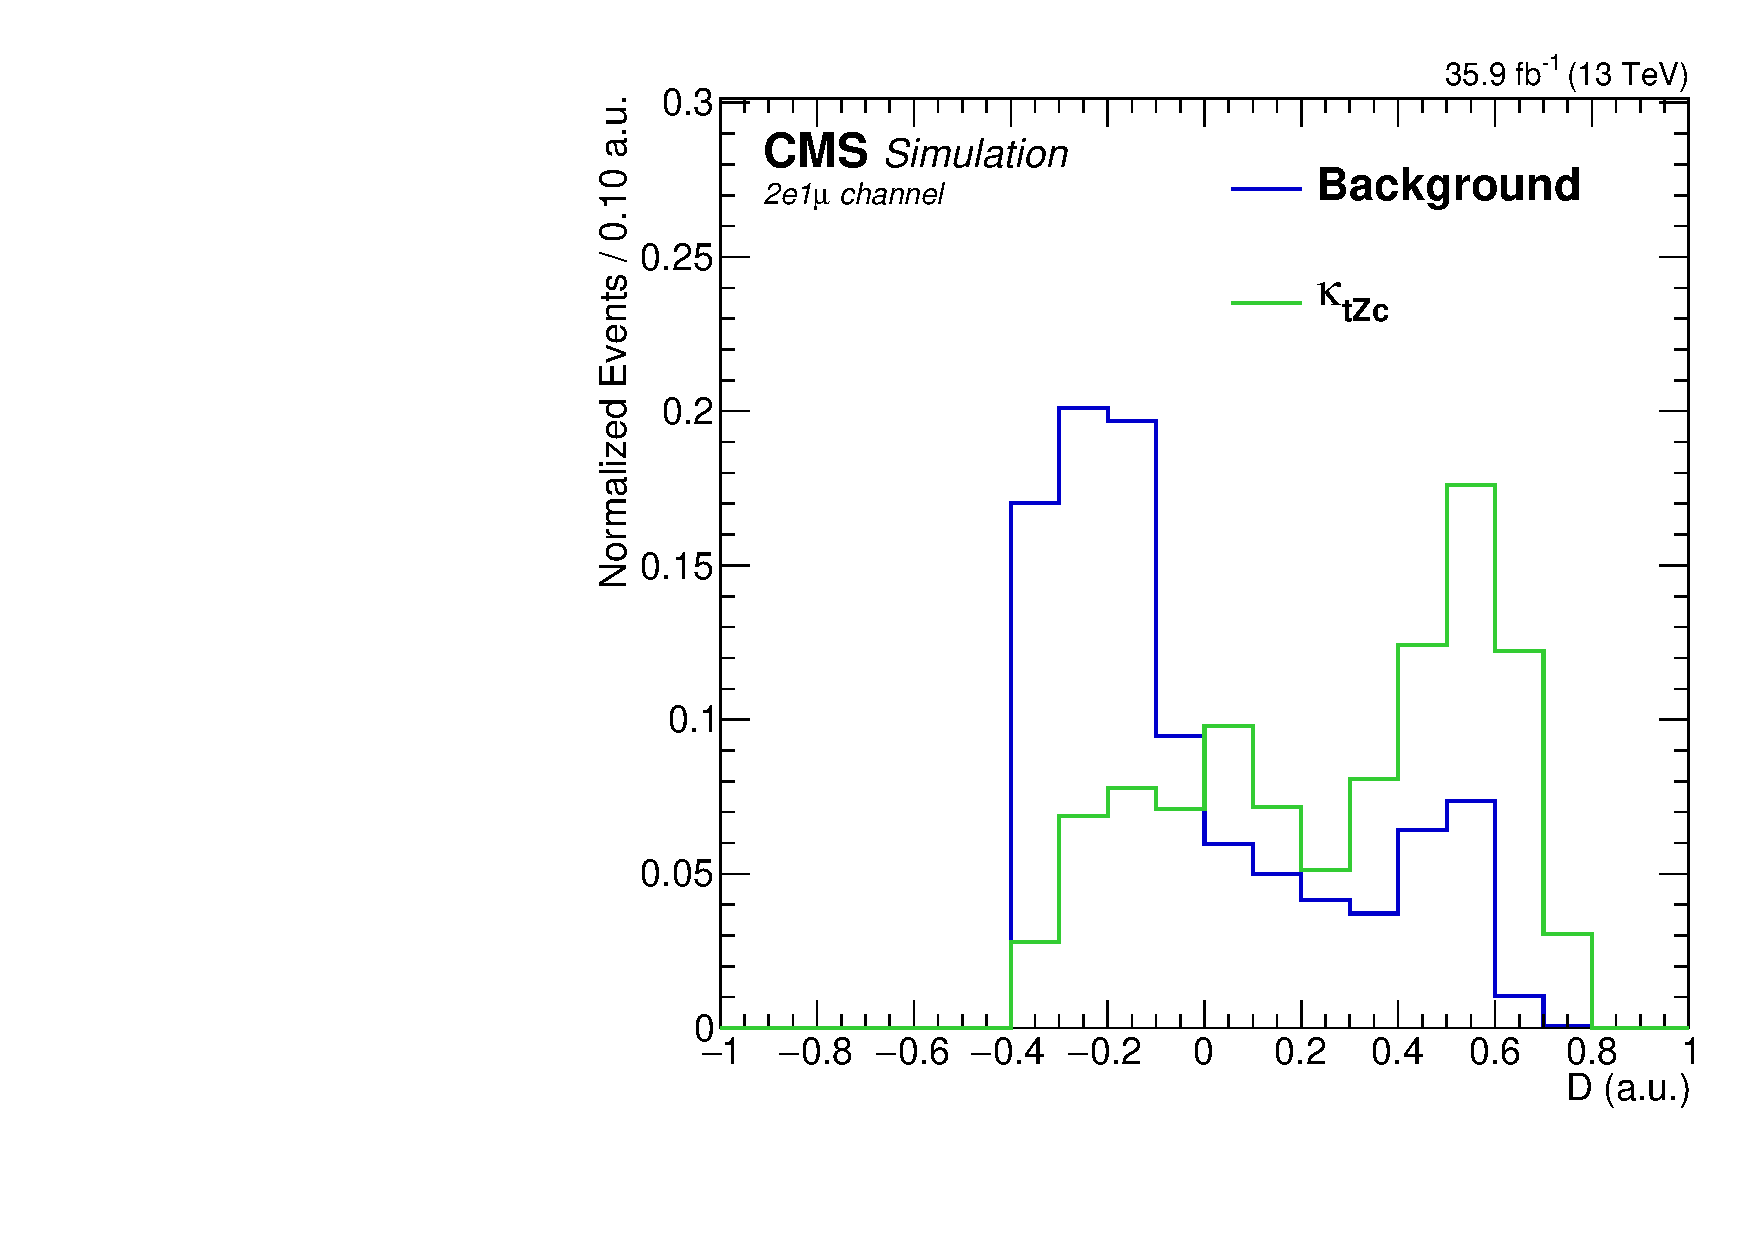
\includegraphics[width=0.49\linewidth]{6_Search/Figures/BDTdistributionsNorm/singletop_Zct_BDT_eeu_Normalized}
	\caption{Normalised distributions of the discriminating variable before the fit, \eemu\ lepton channel. Upper left: \TTSR\ \Zut , upper right: \TTSR\ \Zct ; lower left: \STSR\  \Zut , lower right: \STSR\  \Zct .}
	\label{fig:bdteeunorm}
\end{figure}	

\begin{figure}[htbp]
	\centering
	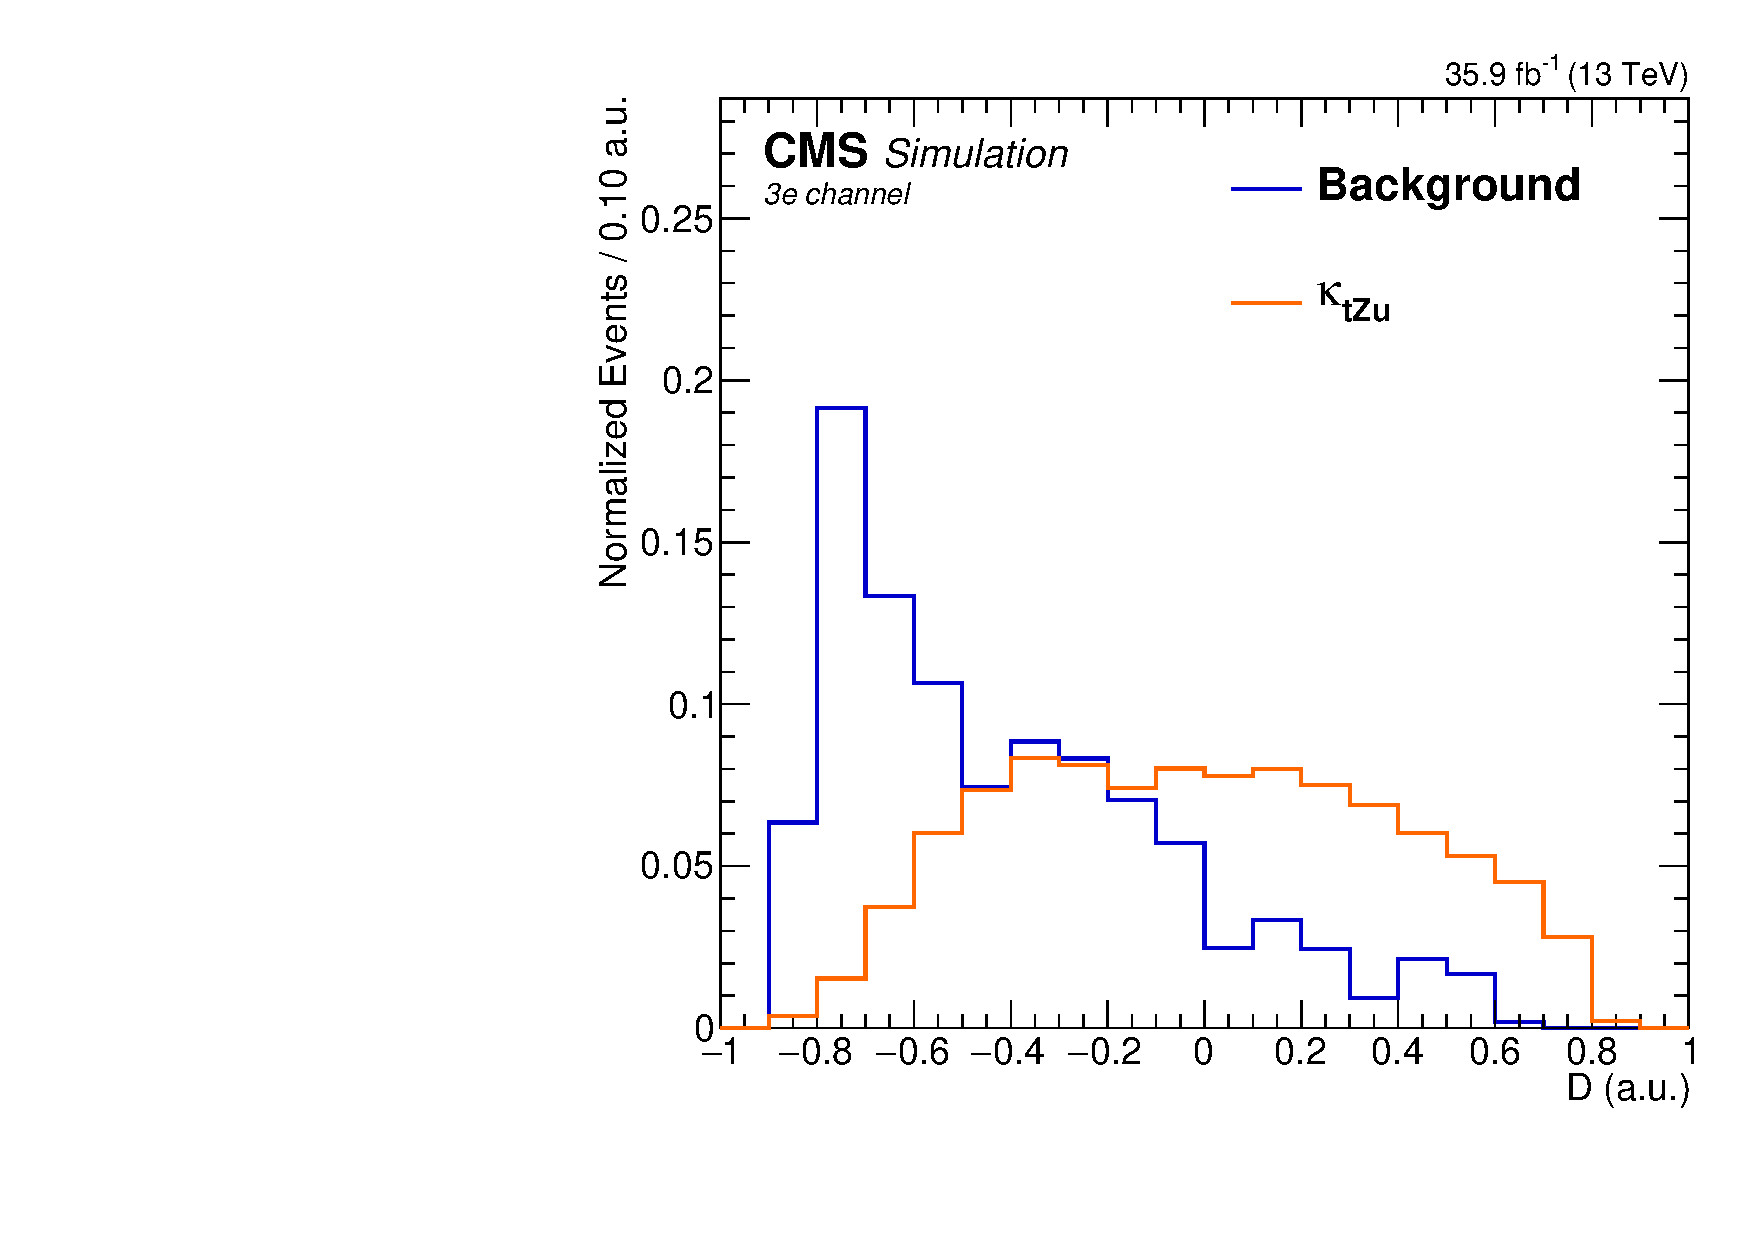
\includegraphics[width=0.49\linewidth]{6_Search/Figures/BDTdistributionsNorm/toppair_Zut_BDT_eee_Normalized}
	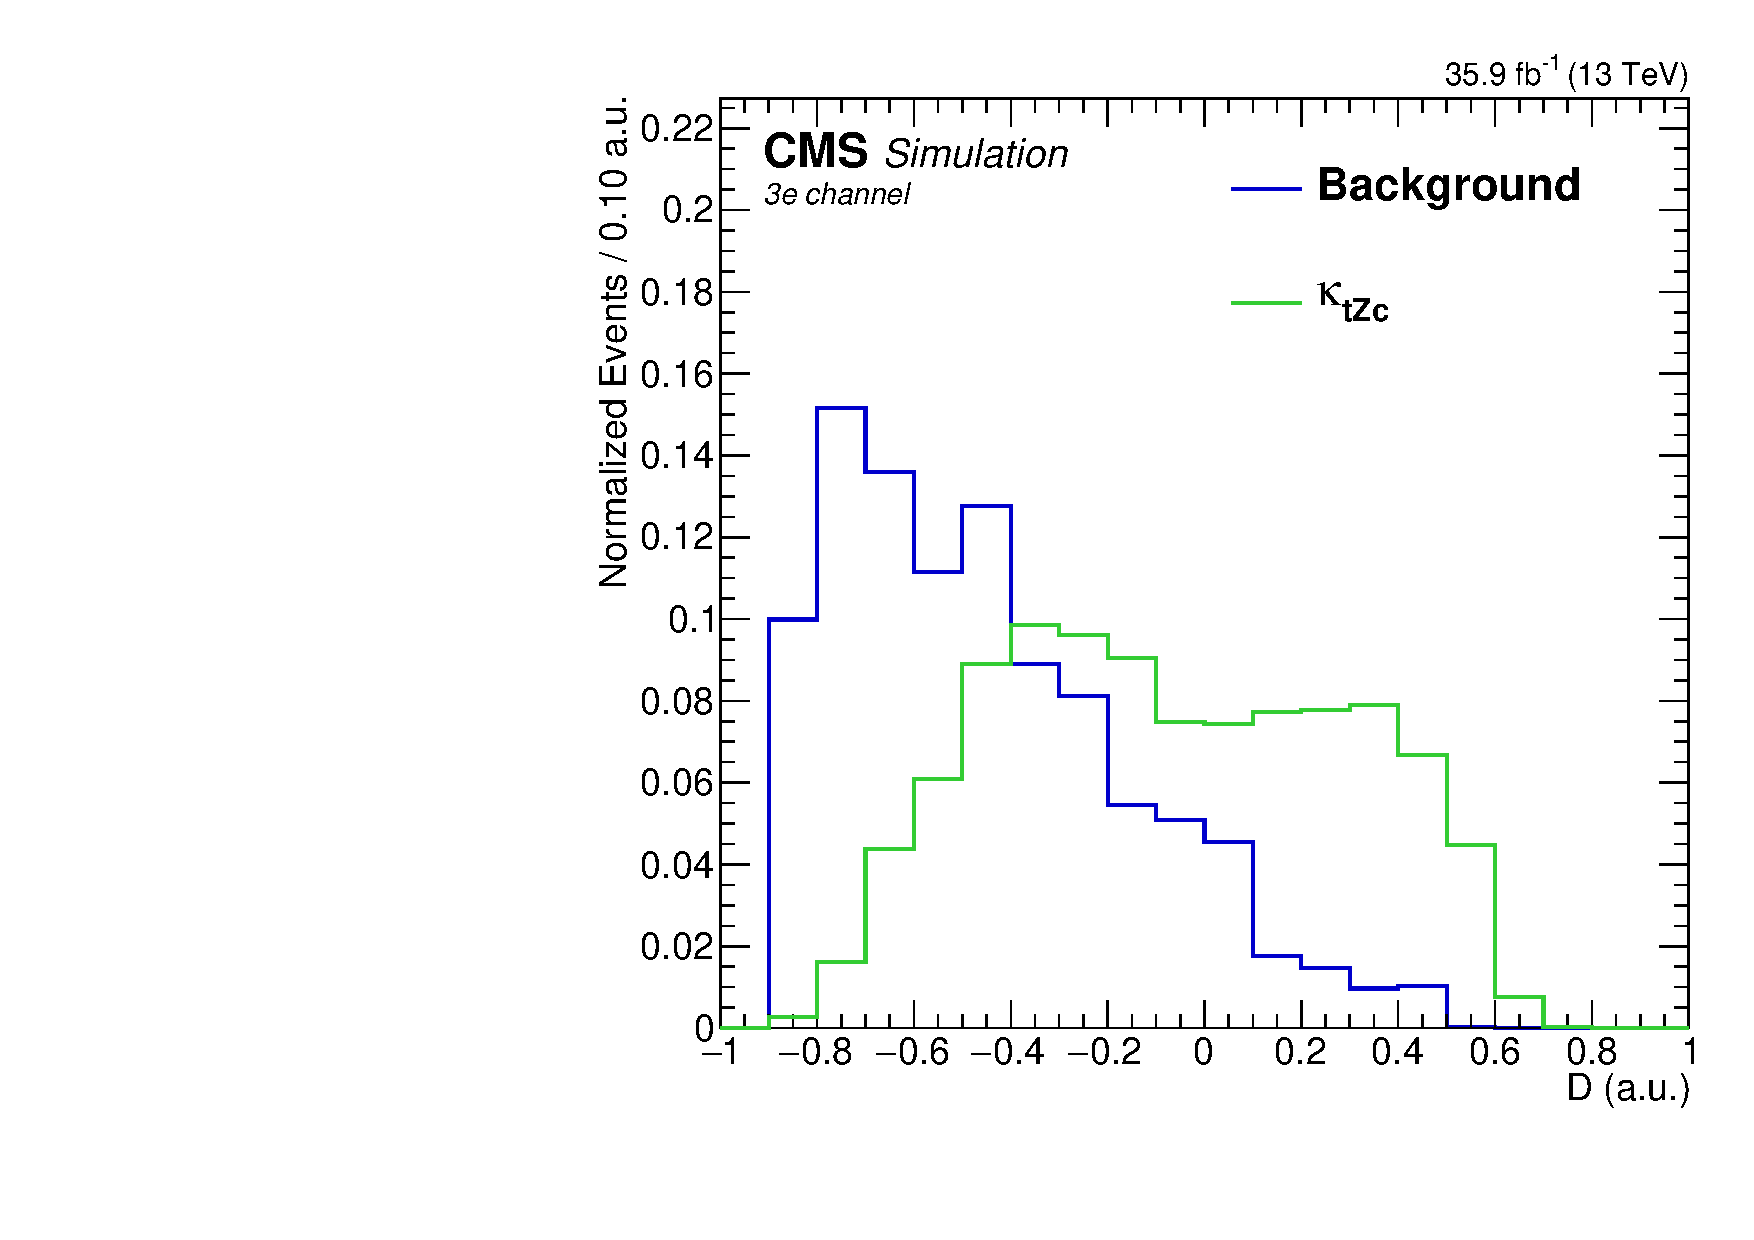
\includegraphics[width=0.49\linewidth]{6_Search/Figures/BDTdistributionsNorm/toppair_Zct_BDT_eee_Normalized}
	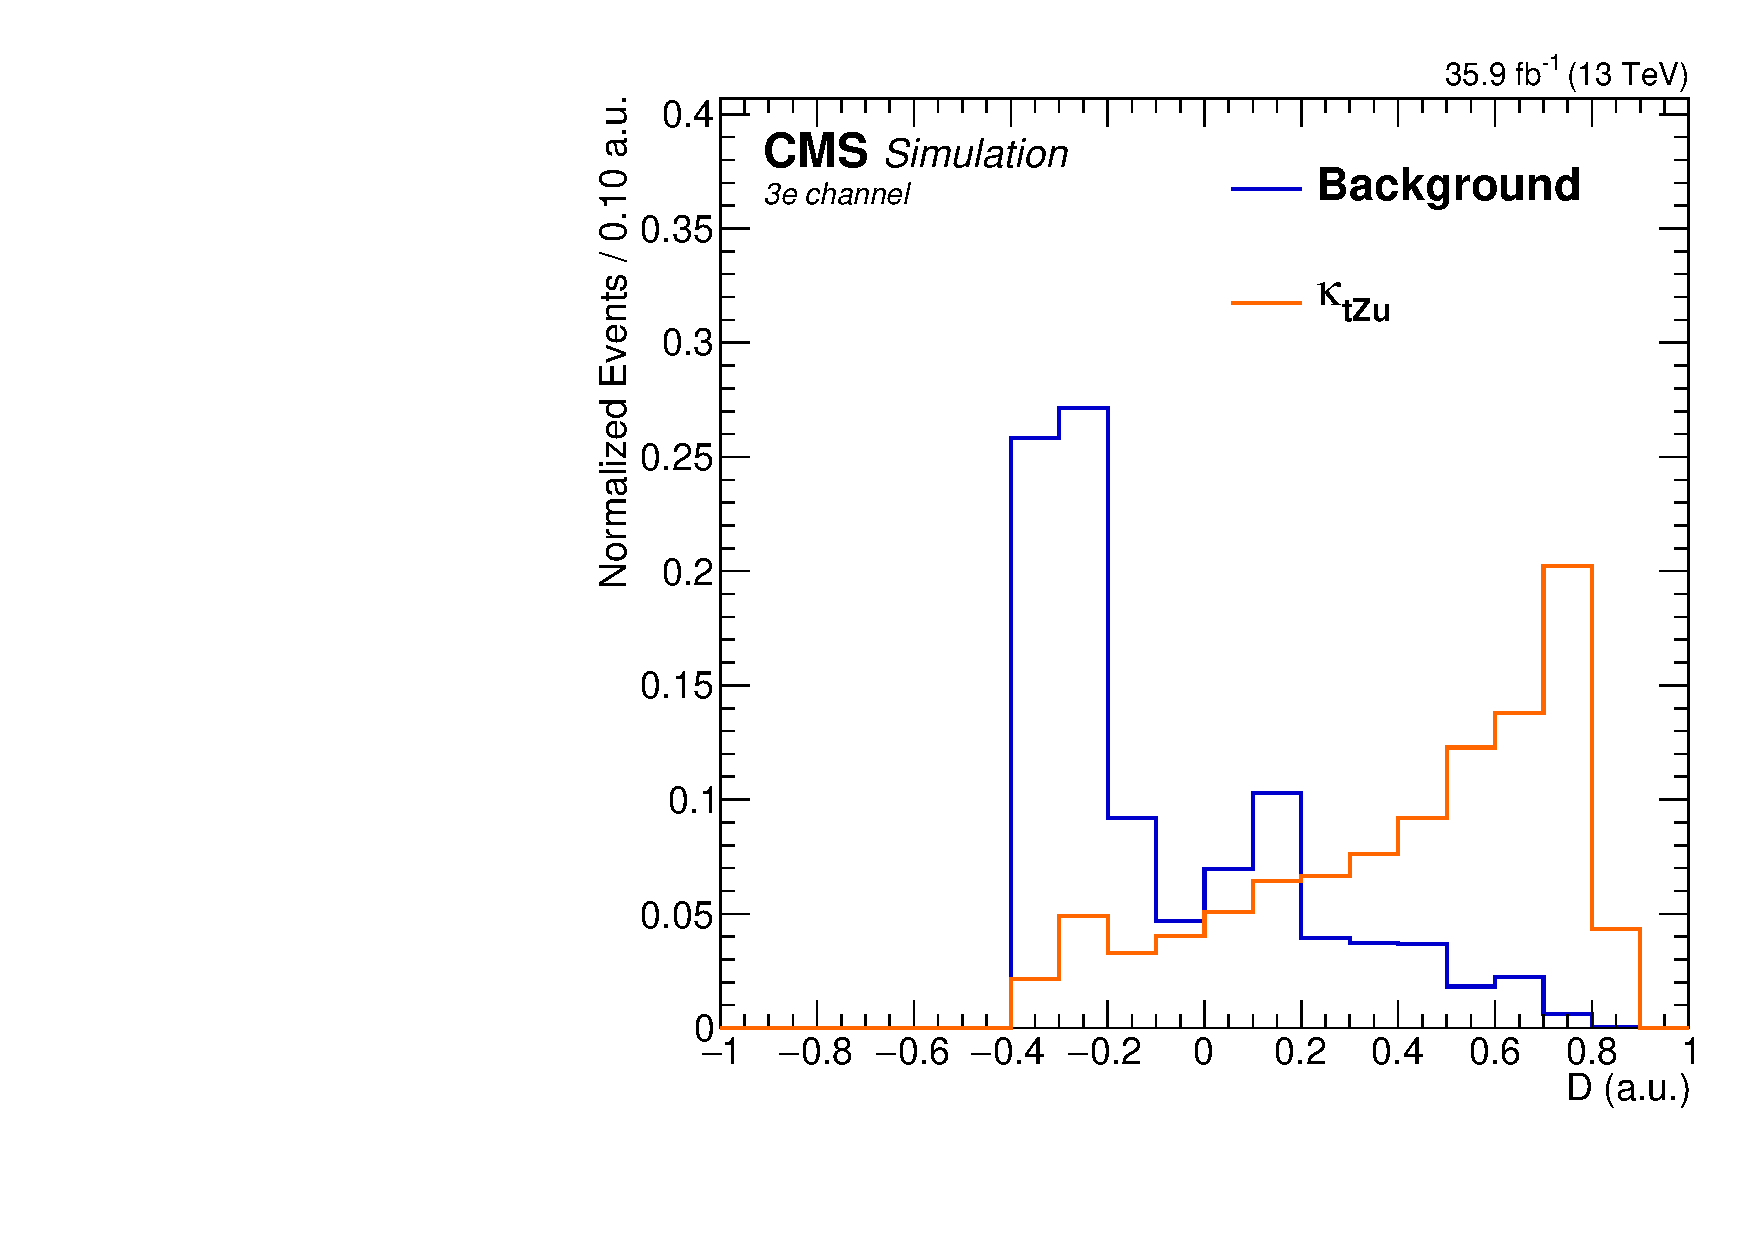
\includegraphics[width=0.49\linewidth]{6_Search/Figures/BDTdistributionsNorm/singletop_Zut_BDT_eee_Normalized}
	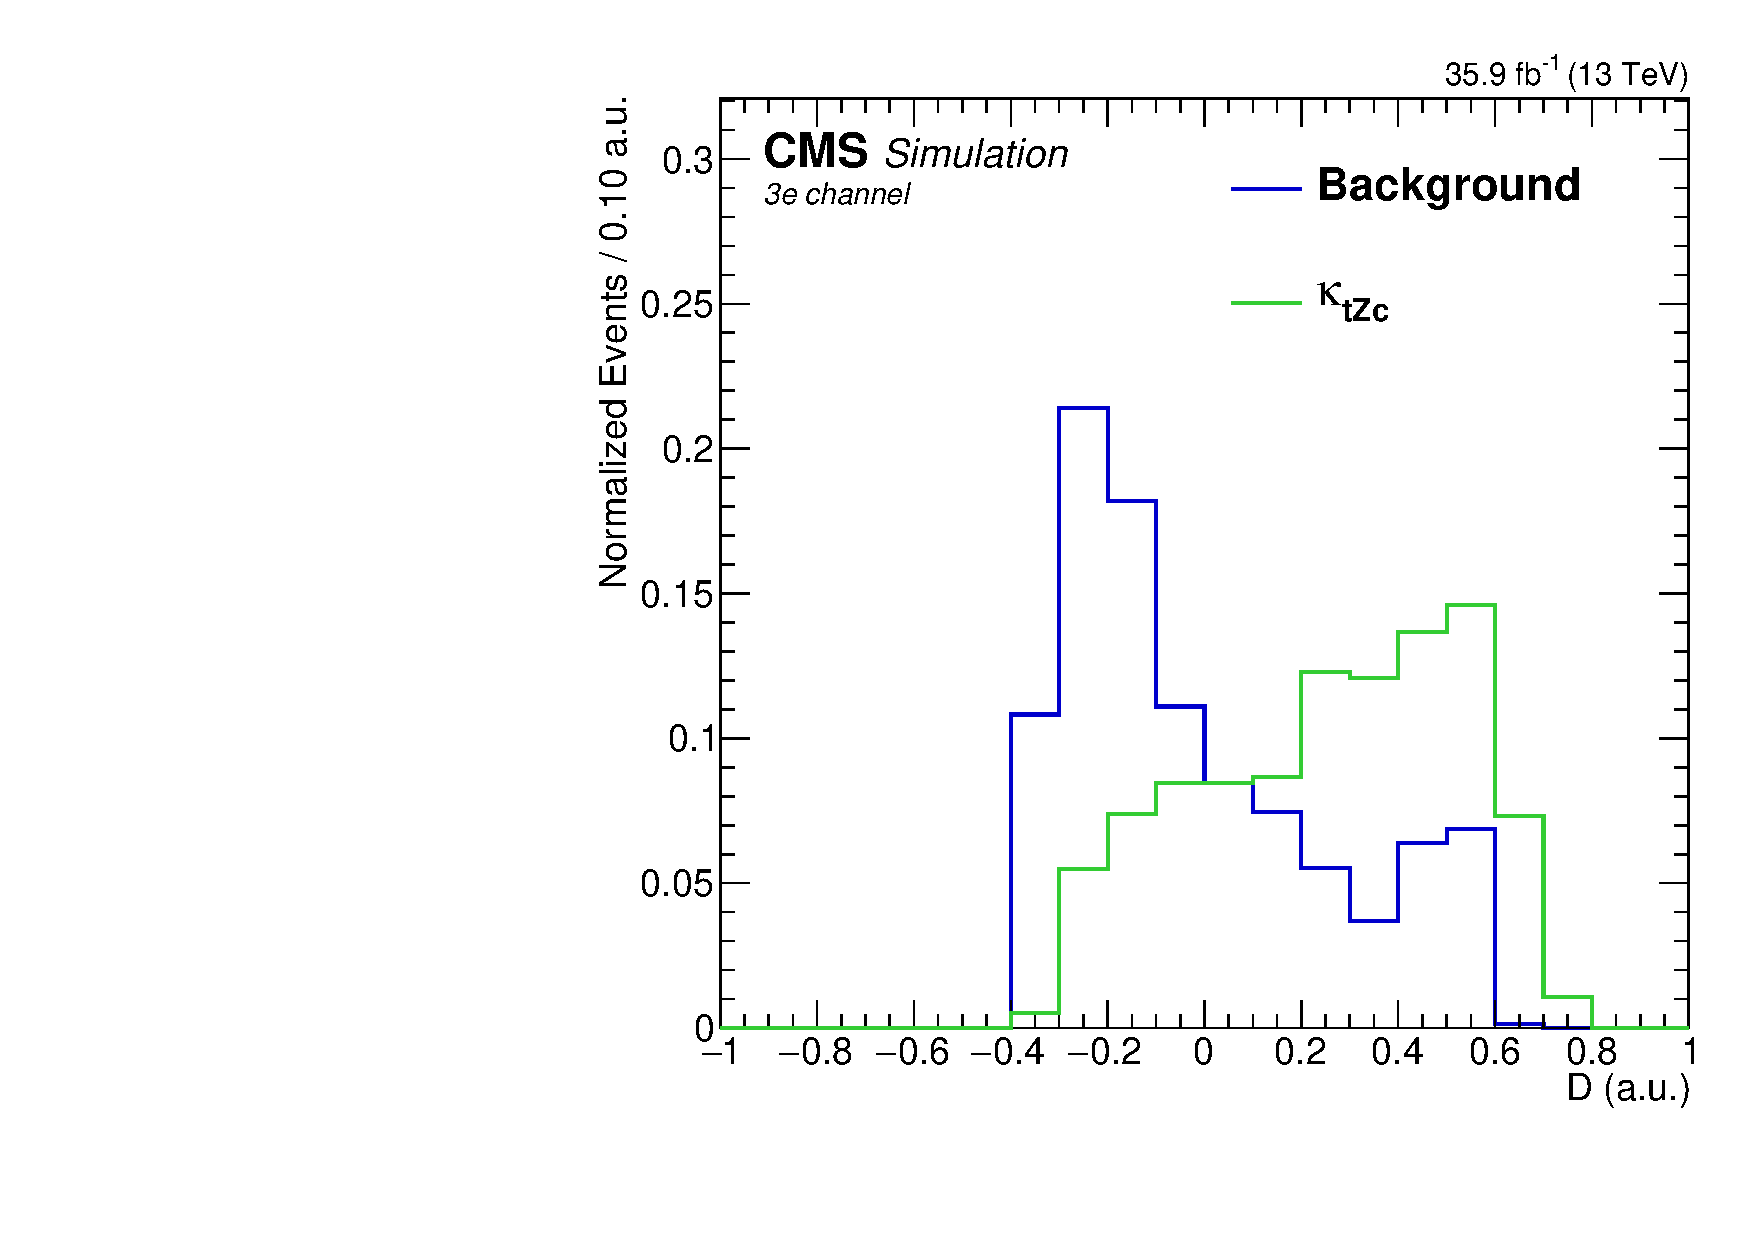
\includegraphics[width=0.49\linewidth]{6_Search/Figures/BDTdistributionsNorm/singletop_Zct_BDT_eee_Normalized}
	\caption{Normalised distributions of the discriminating variable before the fit, \eee\ lepton channel. Upper left: \TTSR\ \Zut , upper right: \TTSR\ \Zct ; lower left: \STSR\  \Zut , lower right: \STSR\  \Zct .}
	\label{fig:bdteeenorm}
\end{figure}	


\begin{figure}[htbp]
	\centering
	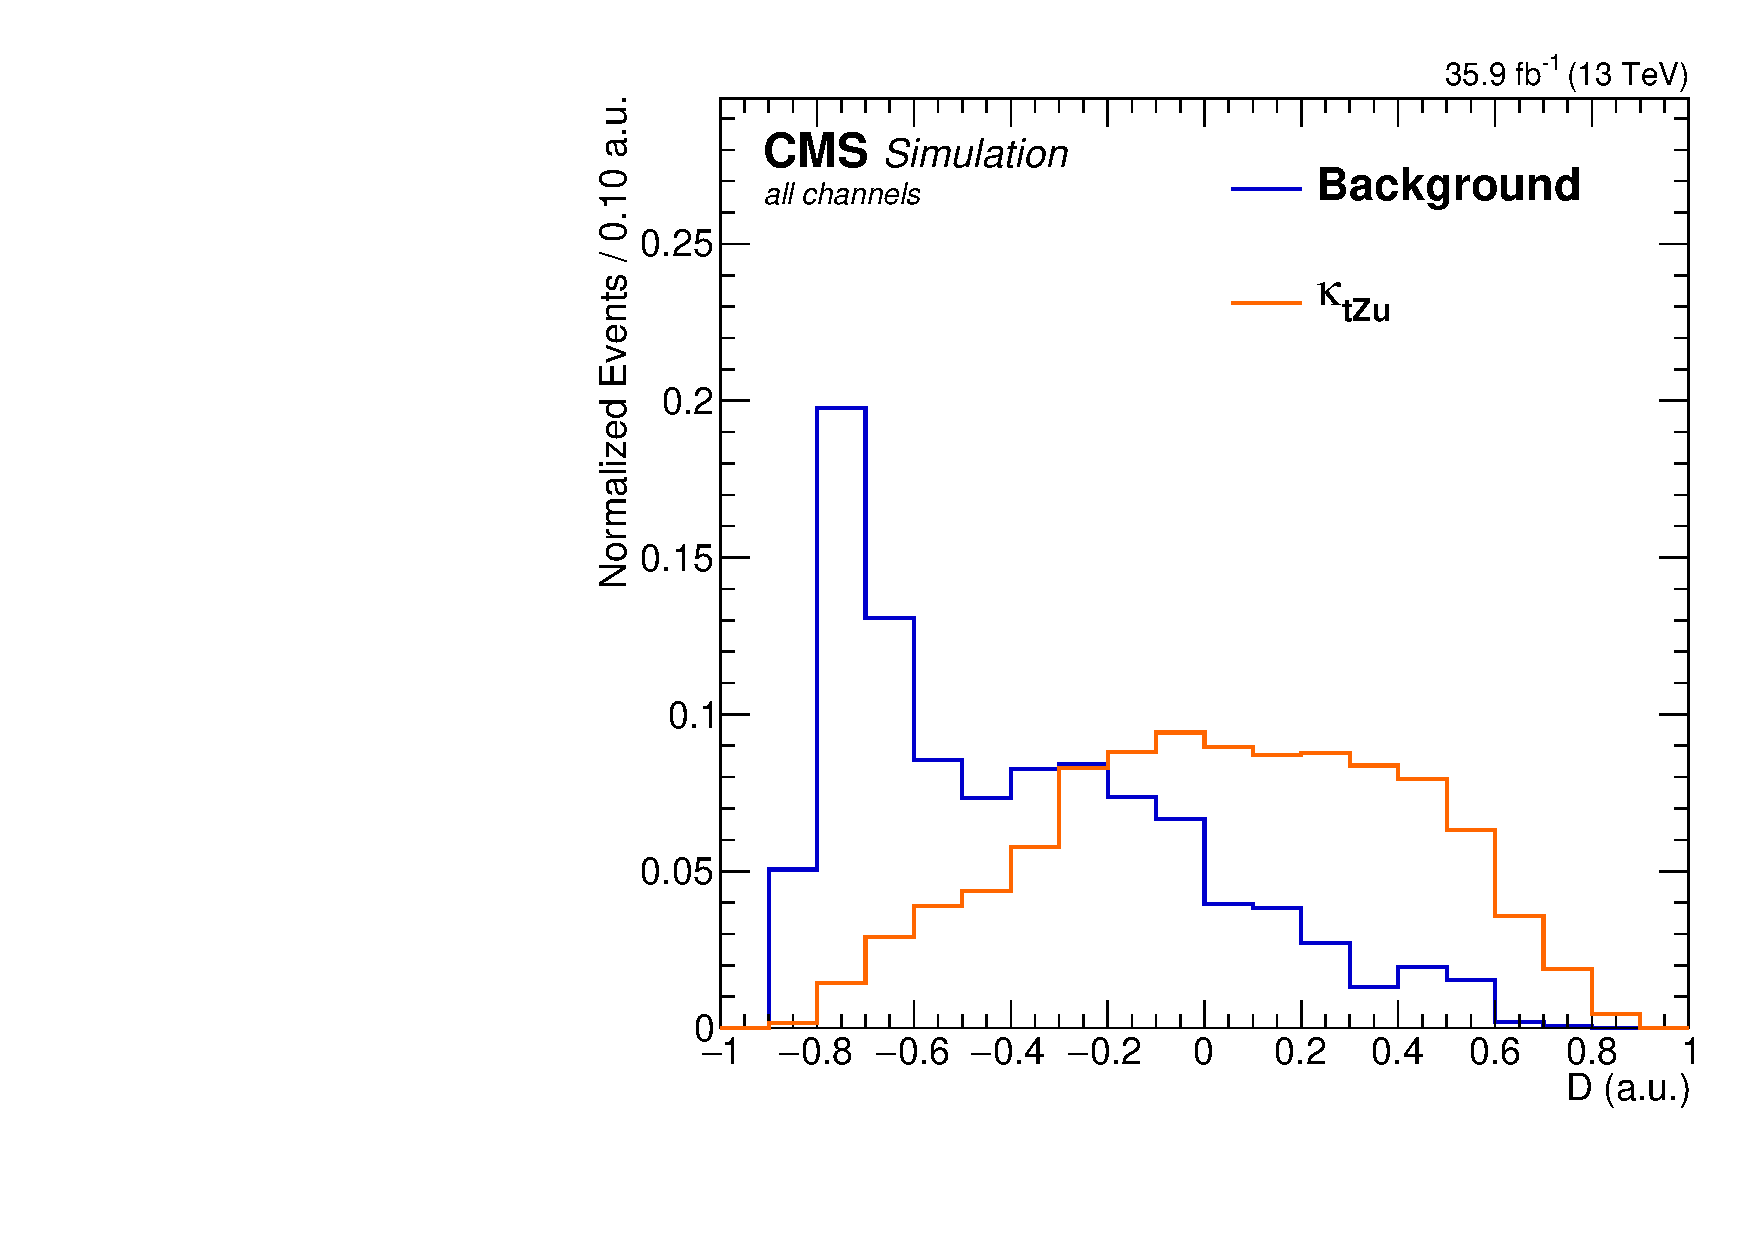
\includegraphics[width=0.49\linewidth]{6_Search/Figures/BDTdistributionsNorm/toppair_Zut_BDT_all_Normalized}
	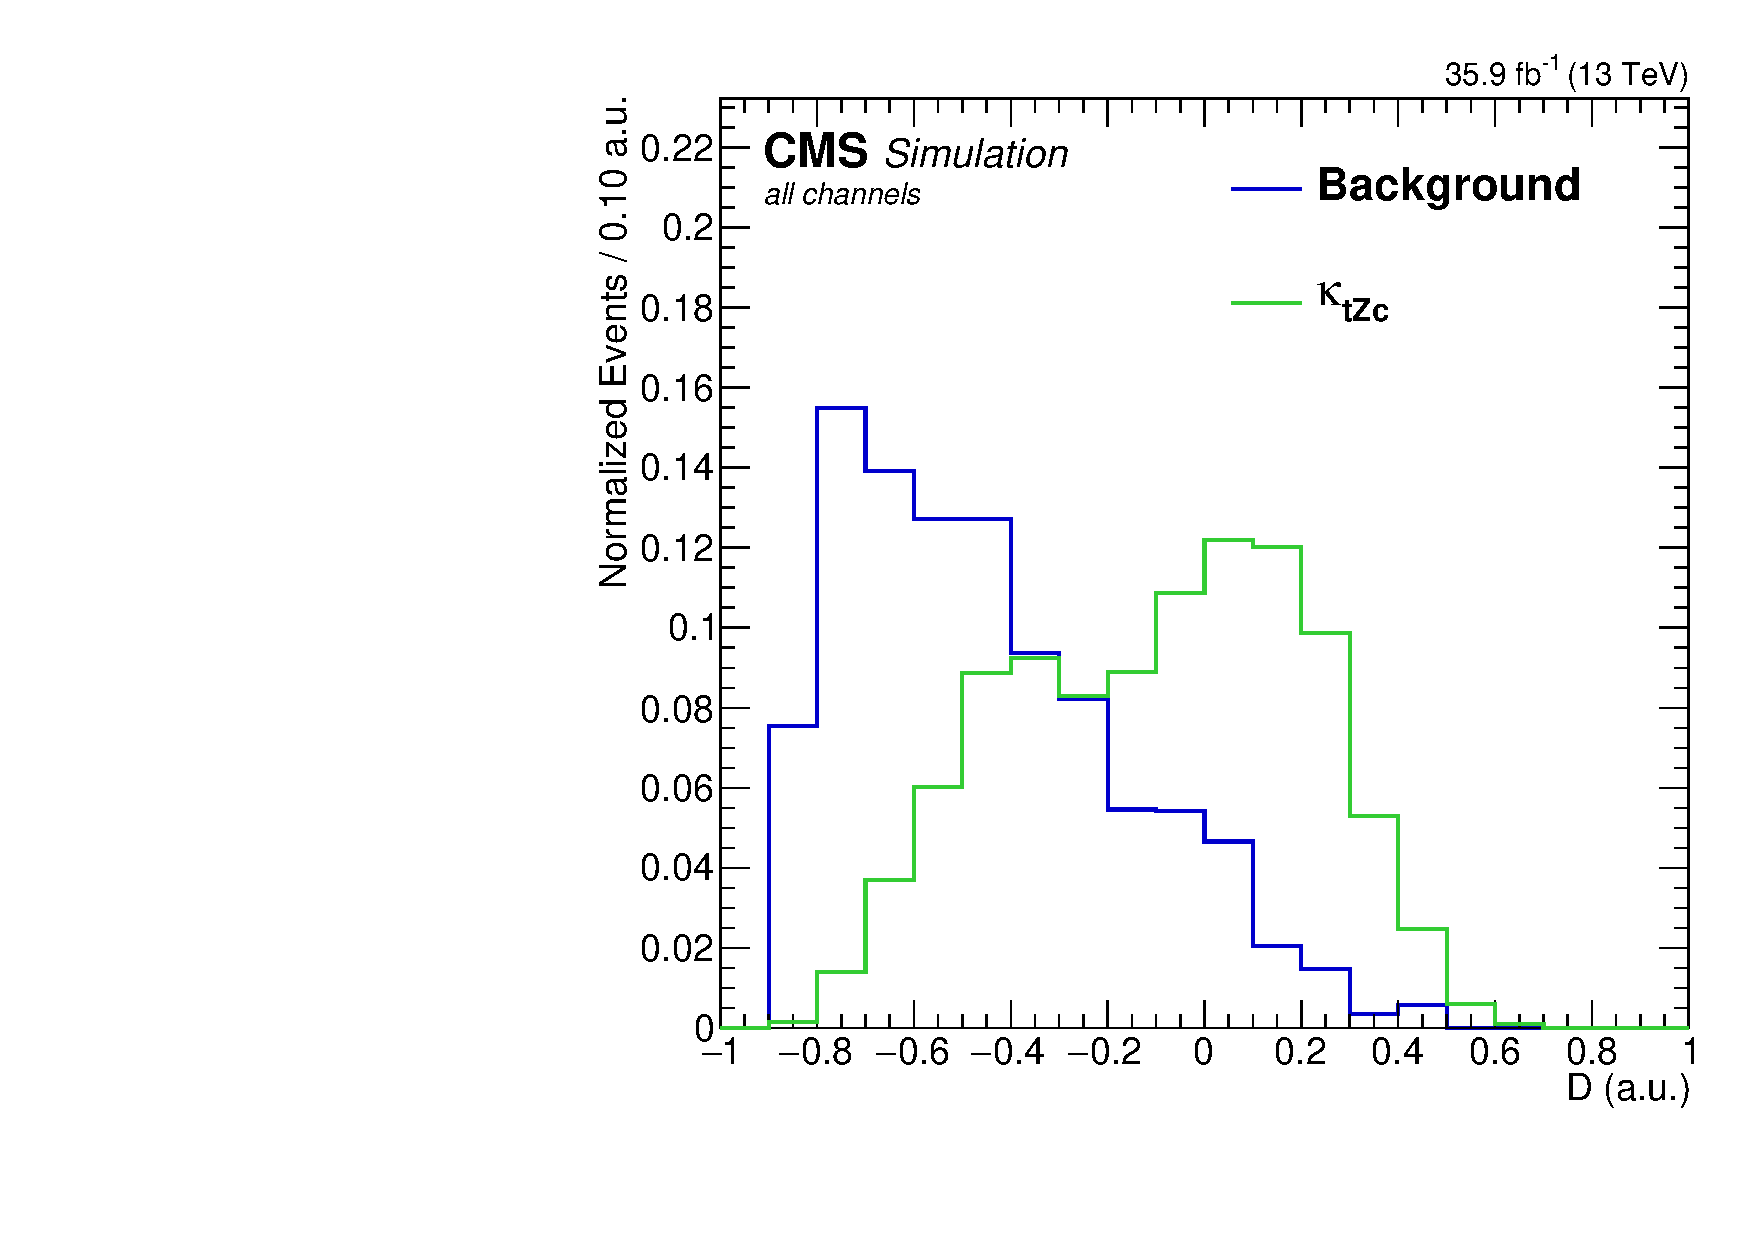
\includegraphics[width=0.49\linewidth]{6_Search/Figures/BDTdistributionsNorm/toppair_Zct_BDT_all_Normalized}
	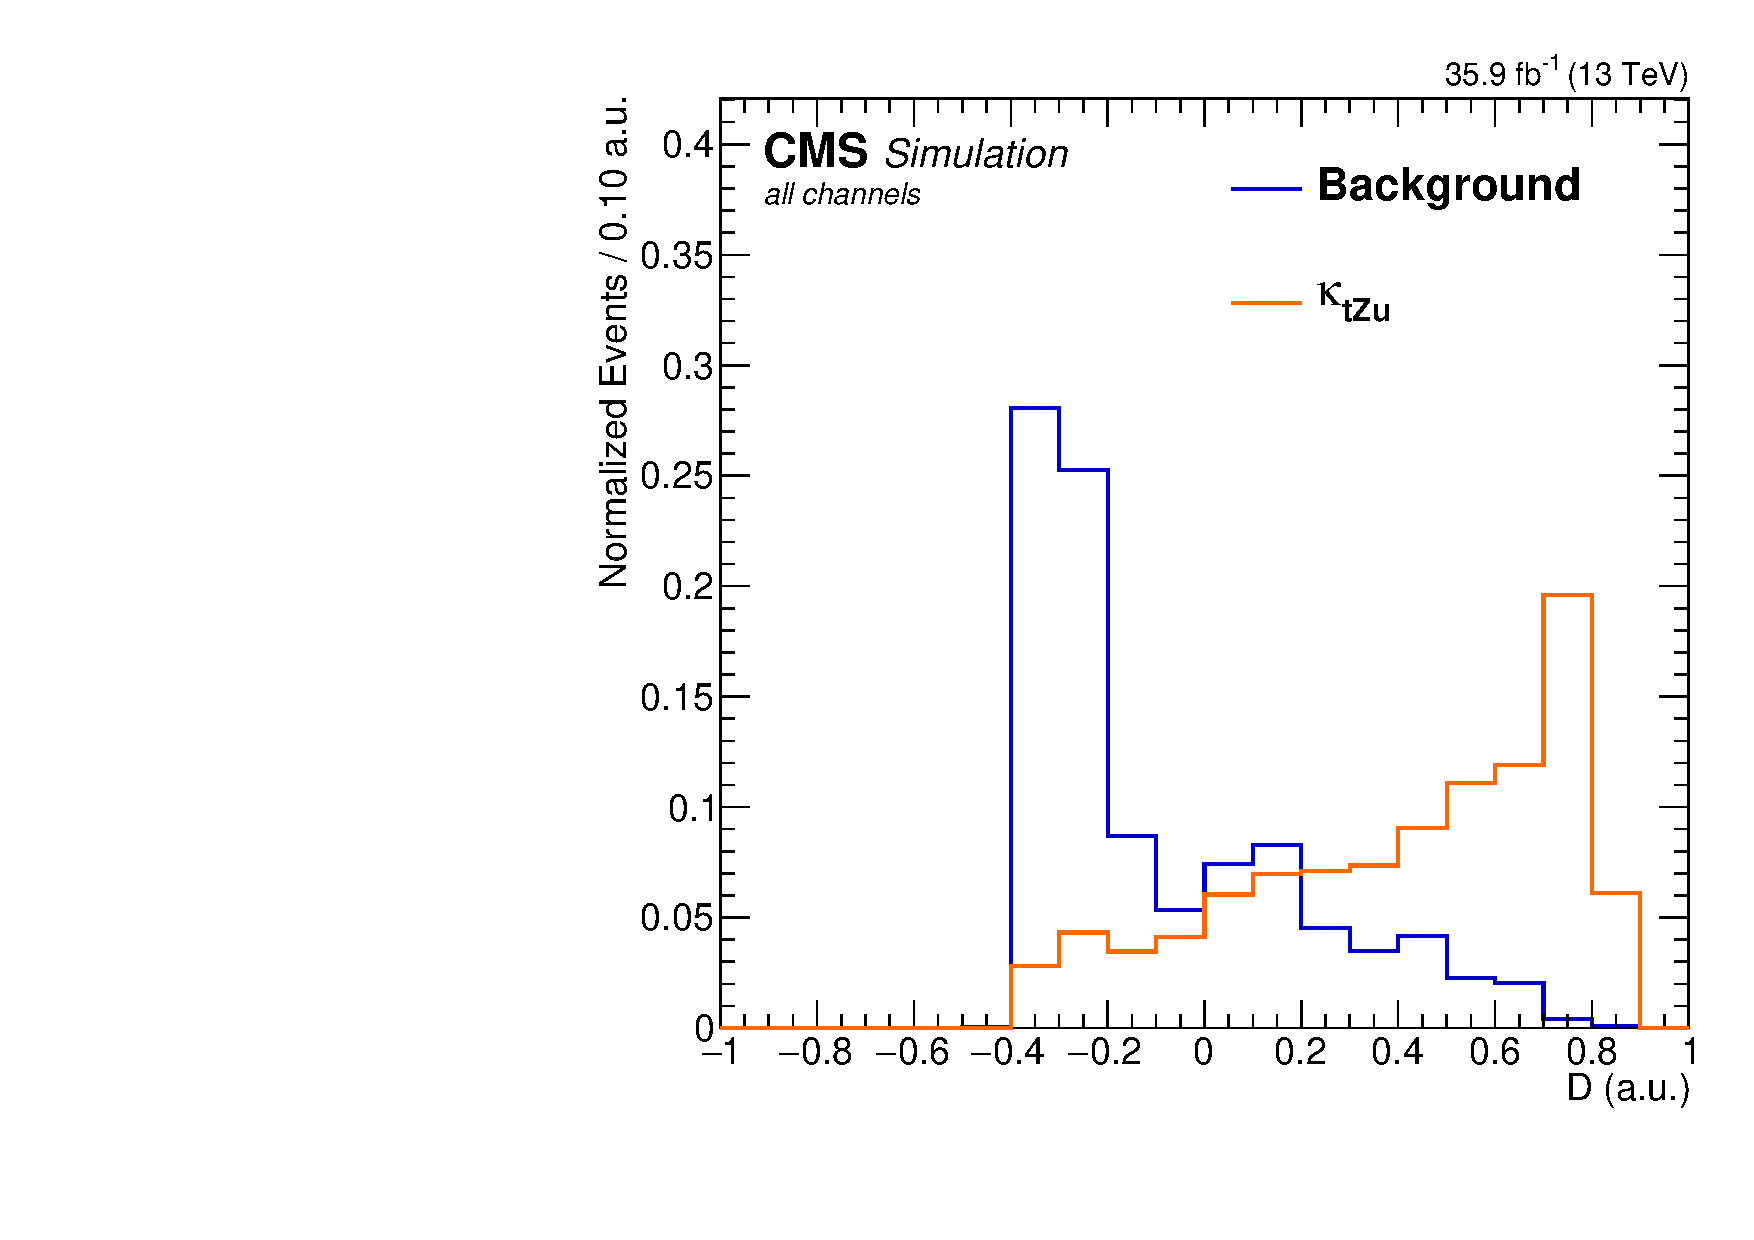
\includegraphics[width=0.49\linewidth]{6_Search/Figures/BDTdistributionsNorm/singletop_Zut_BDT_all_Normalized}
	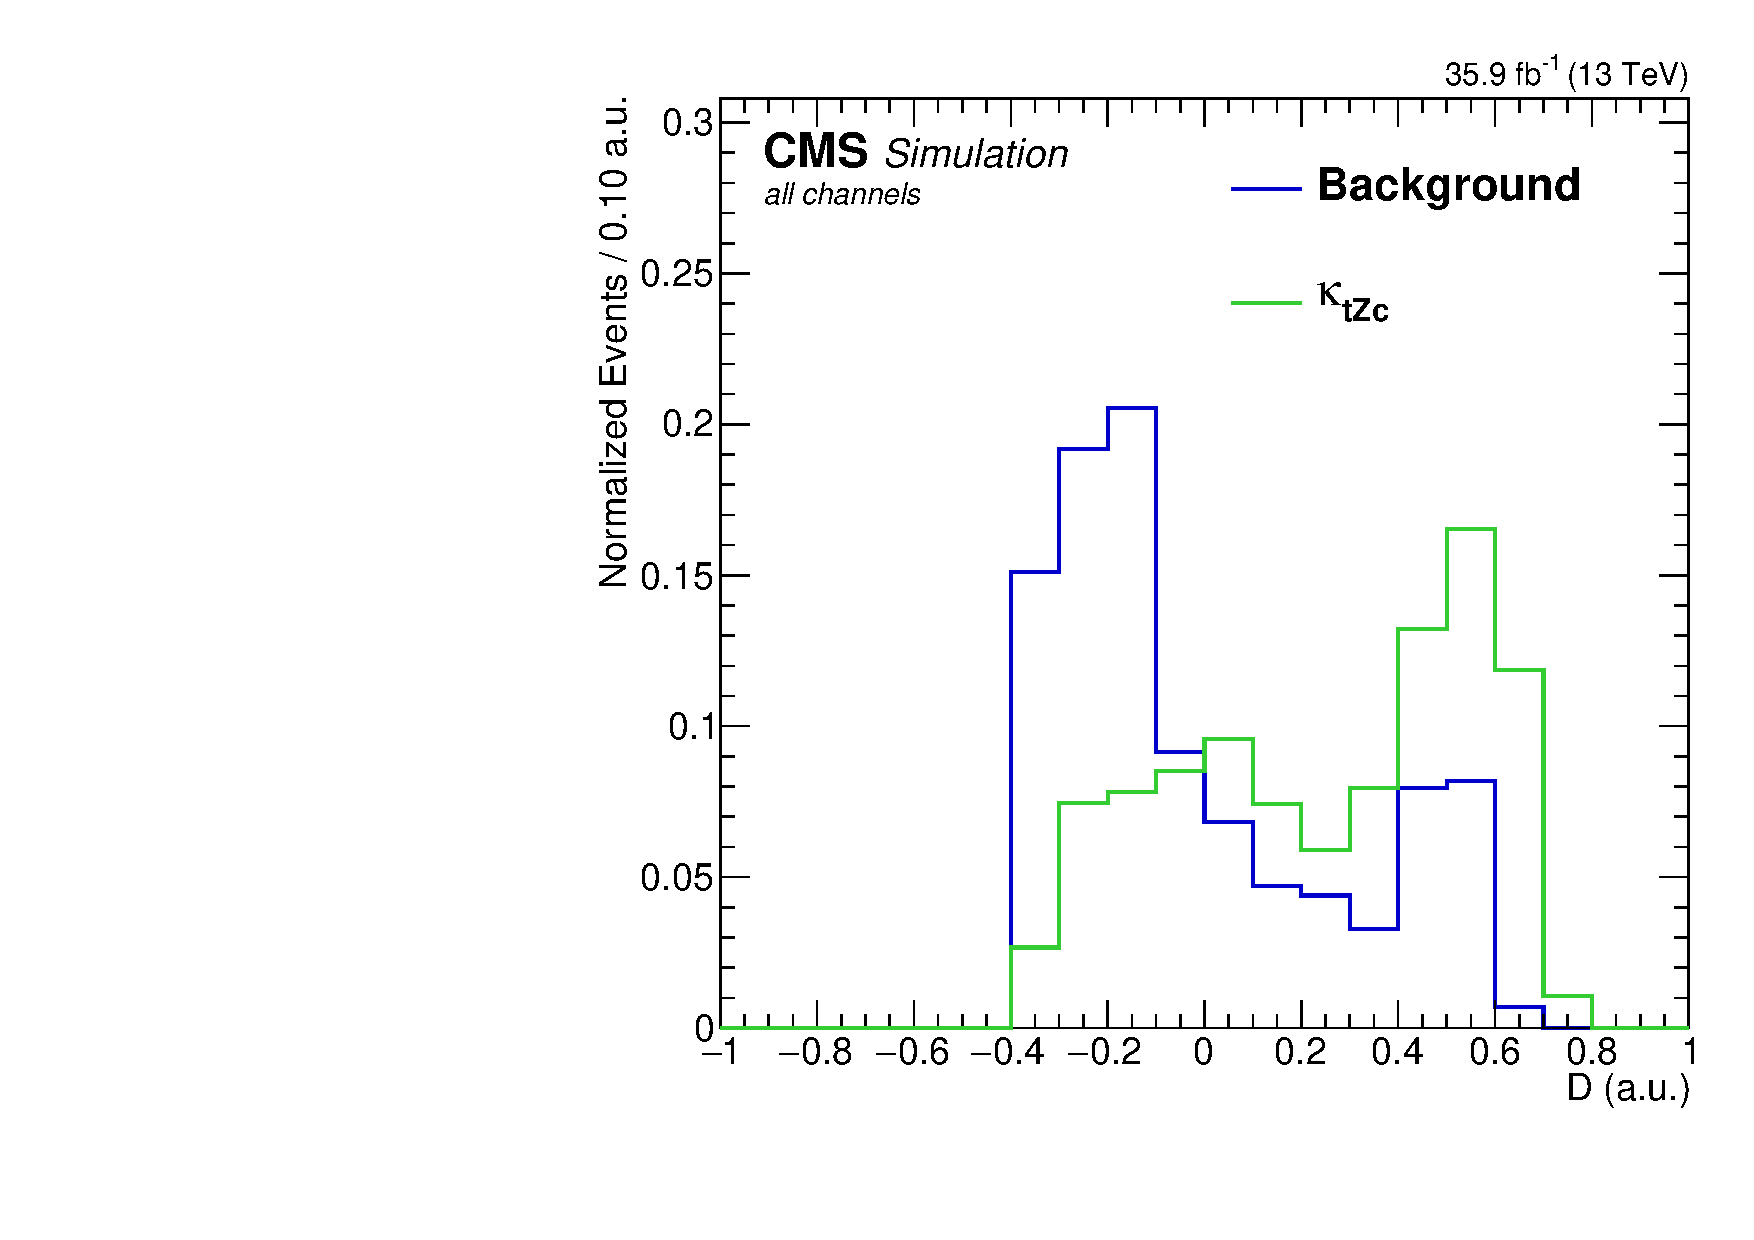
\includegraphics[width=0.49\linewidth]{6_Search/Figures/BDTdistributionsNorm/singletop_Zct_BDT_all_Normalized}
	\caption{Normalised distributions of the discriminating variable before the fit, all different lepton channels together. Upper left: \TTSR\ \Zut , upper right: \TTSR\ \Zct ; lower left: \STSR\  \Zut , lower right: \STSR\  \Zct .}
	\label{fig:bdtallnorm}
\end{figure}	

%\begin{figure}[htbp]
%	\centering
%	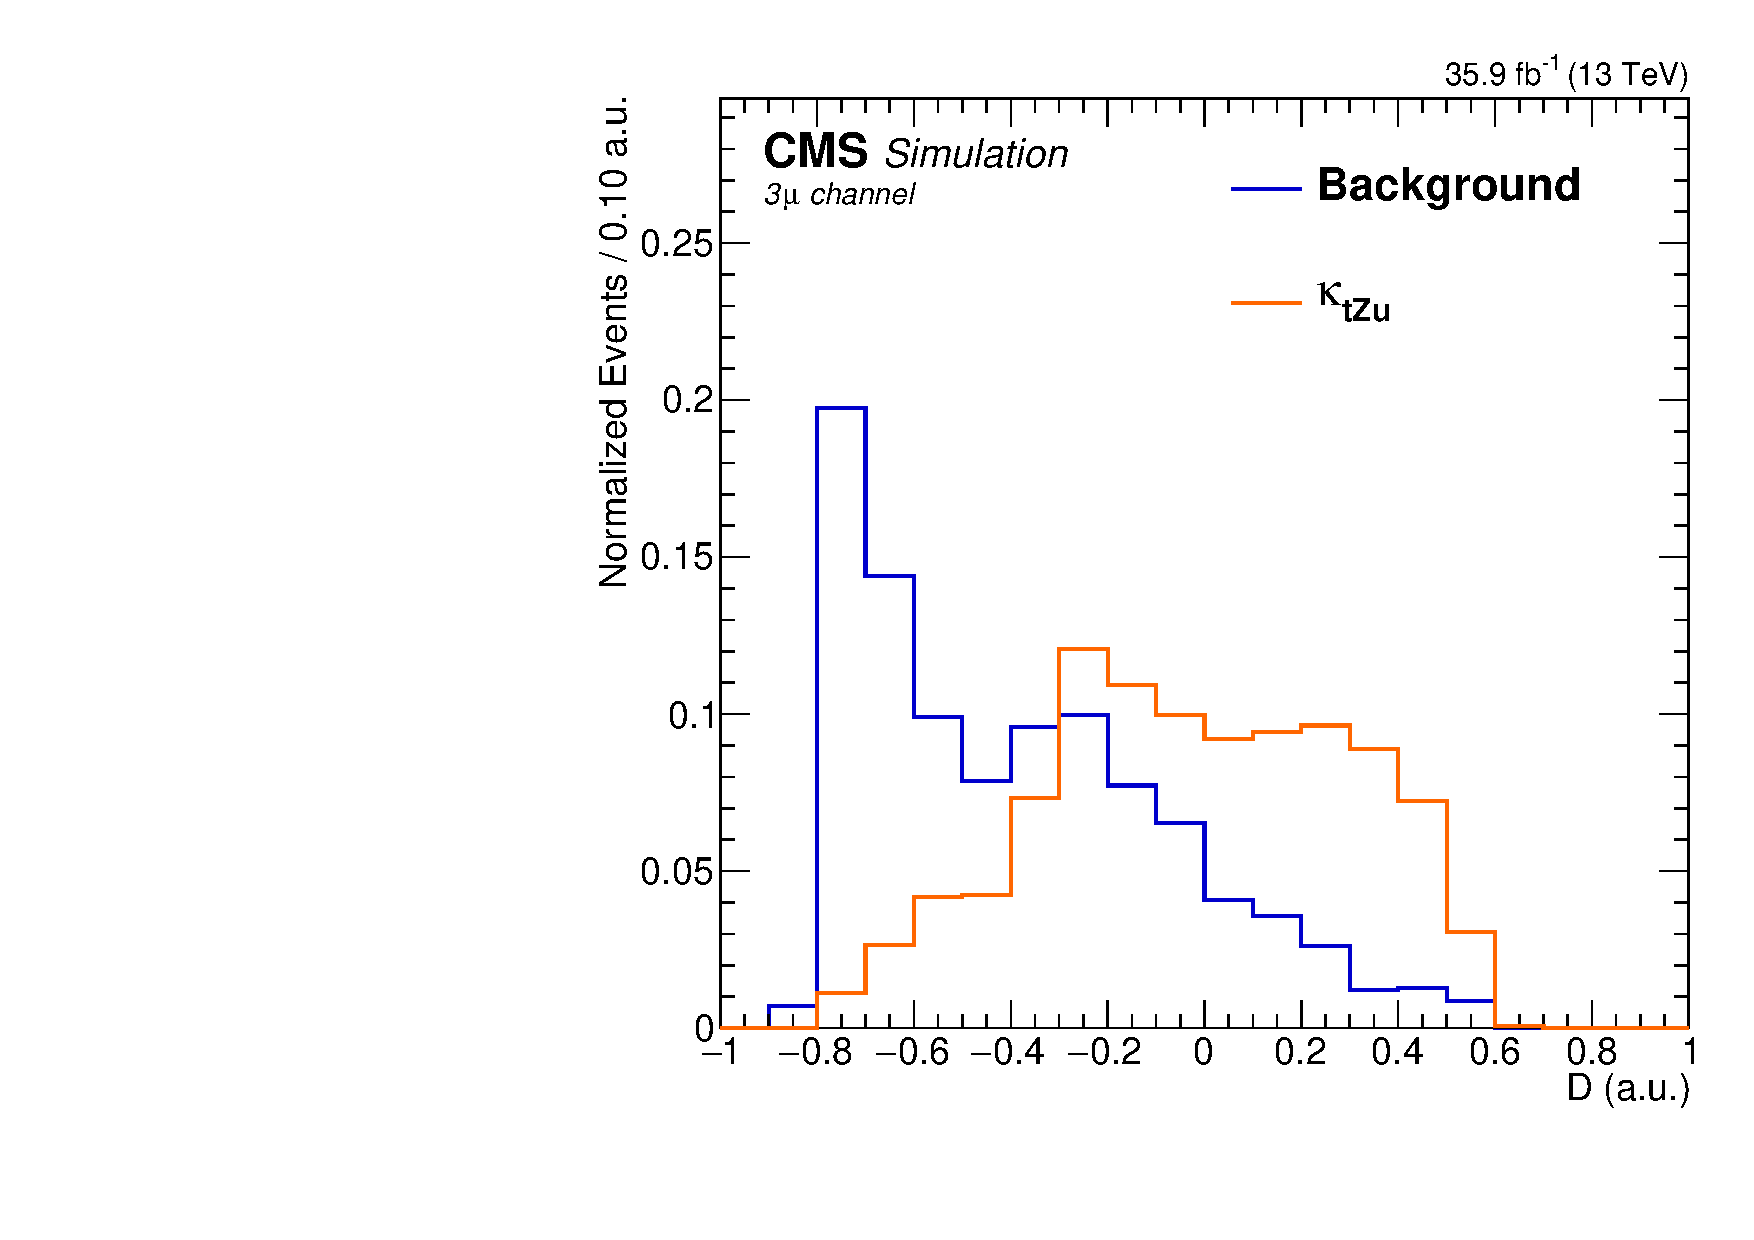
\includegraphics[width=0.24\linewidth]{6_Search/Figures/BDTdistributionsNorm/toppair_Zut_BDT_uuu_Normalized}
%	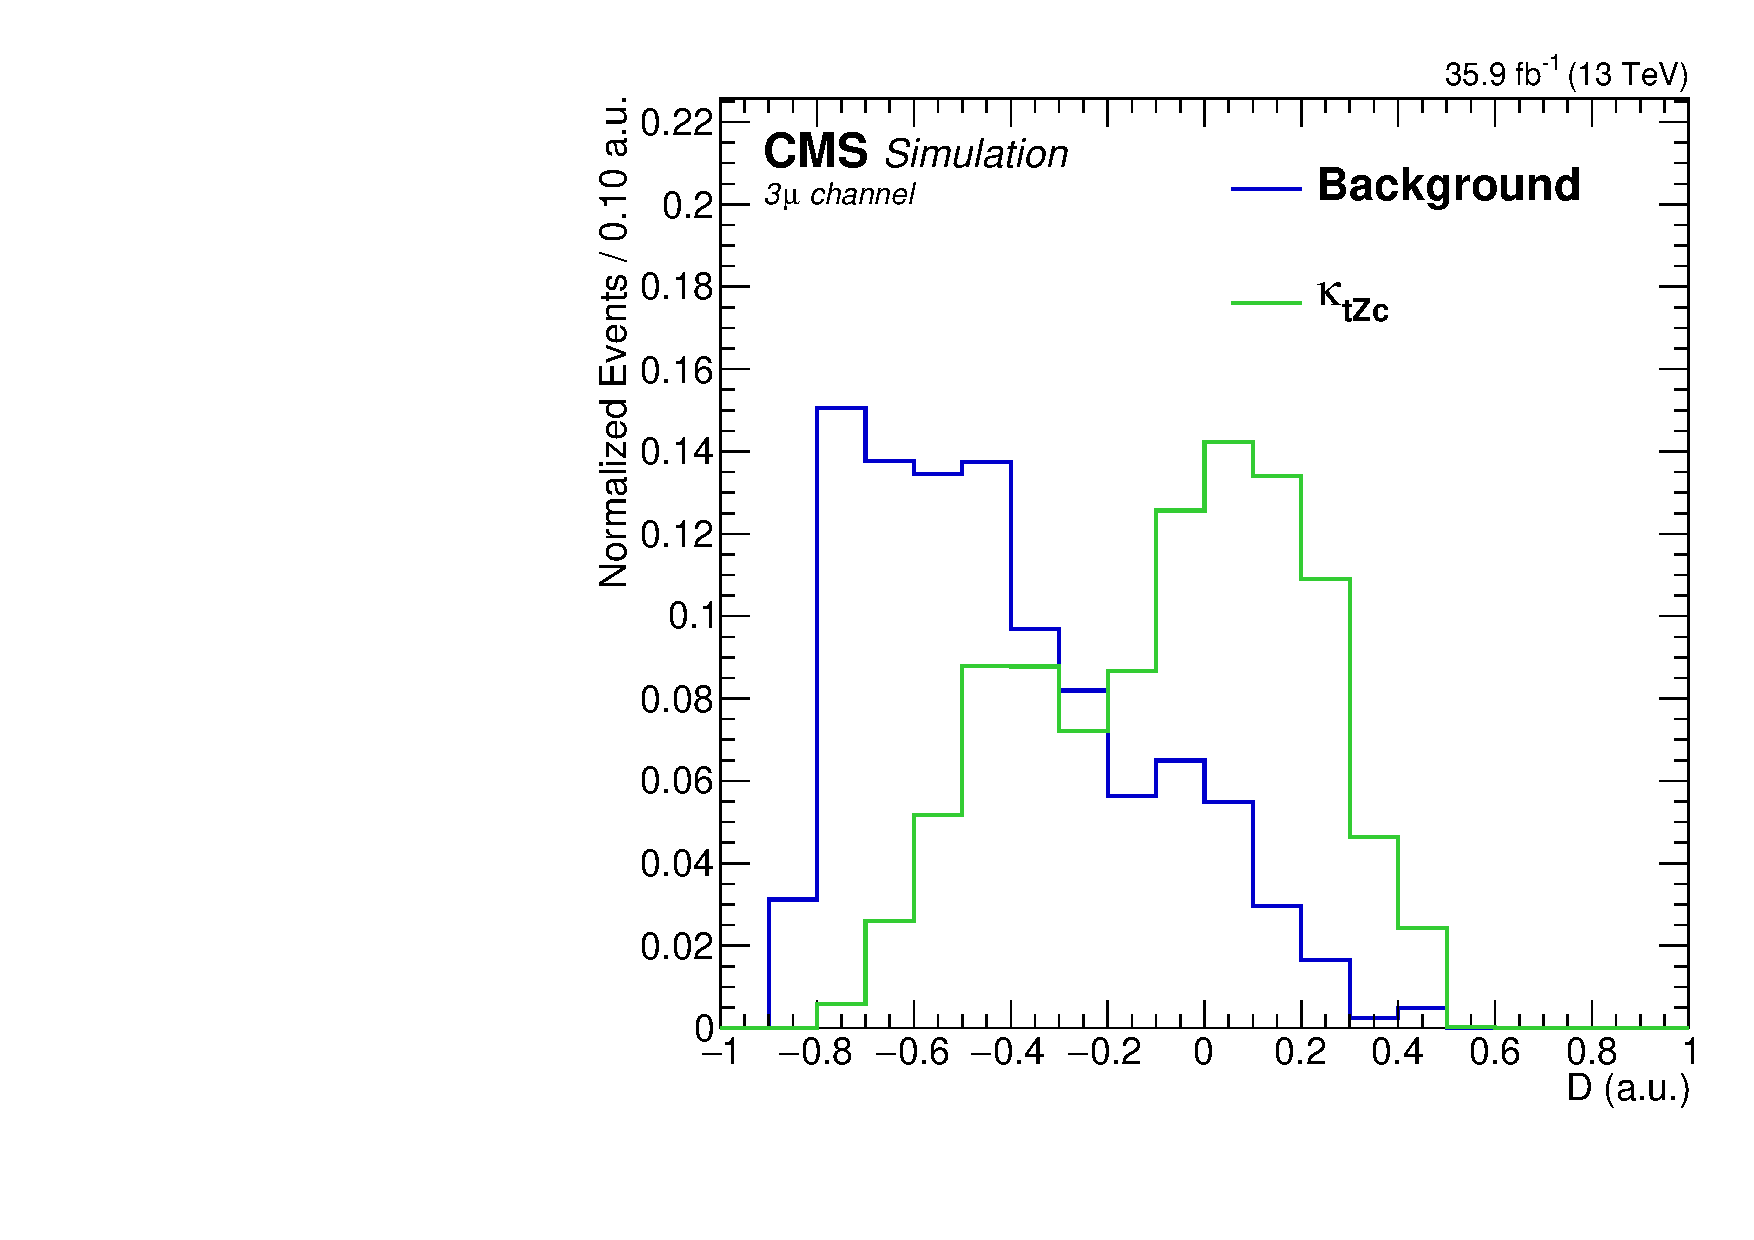
\includegraphics[width=0.24\linewidth]{6_Search/Figures/BDTdistributionsNorm/toppair_Zct_BDT_uuu_Normalized}
%	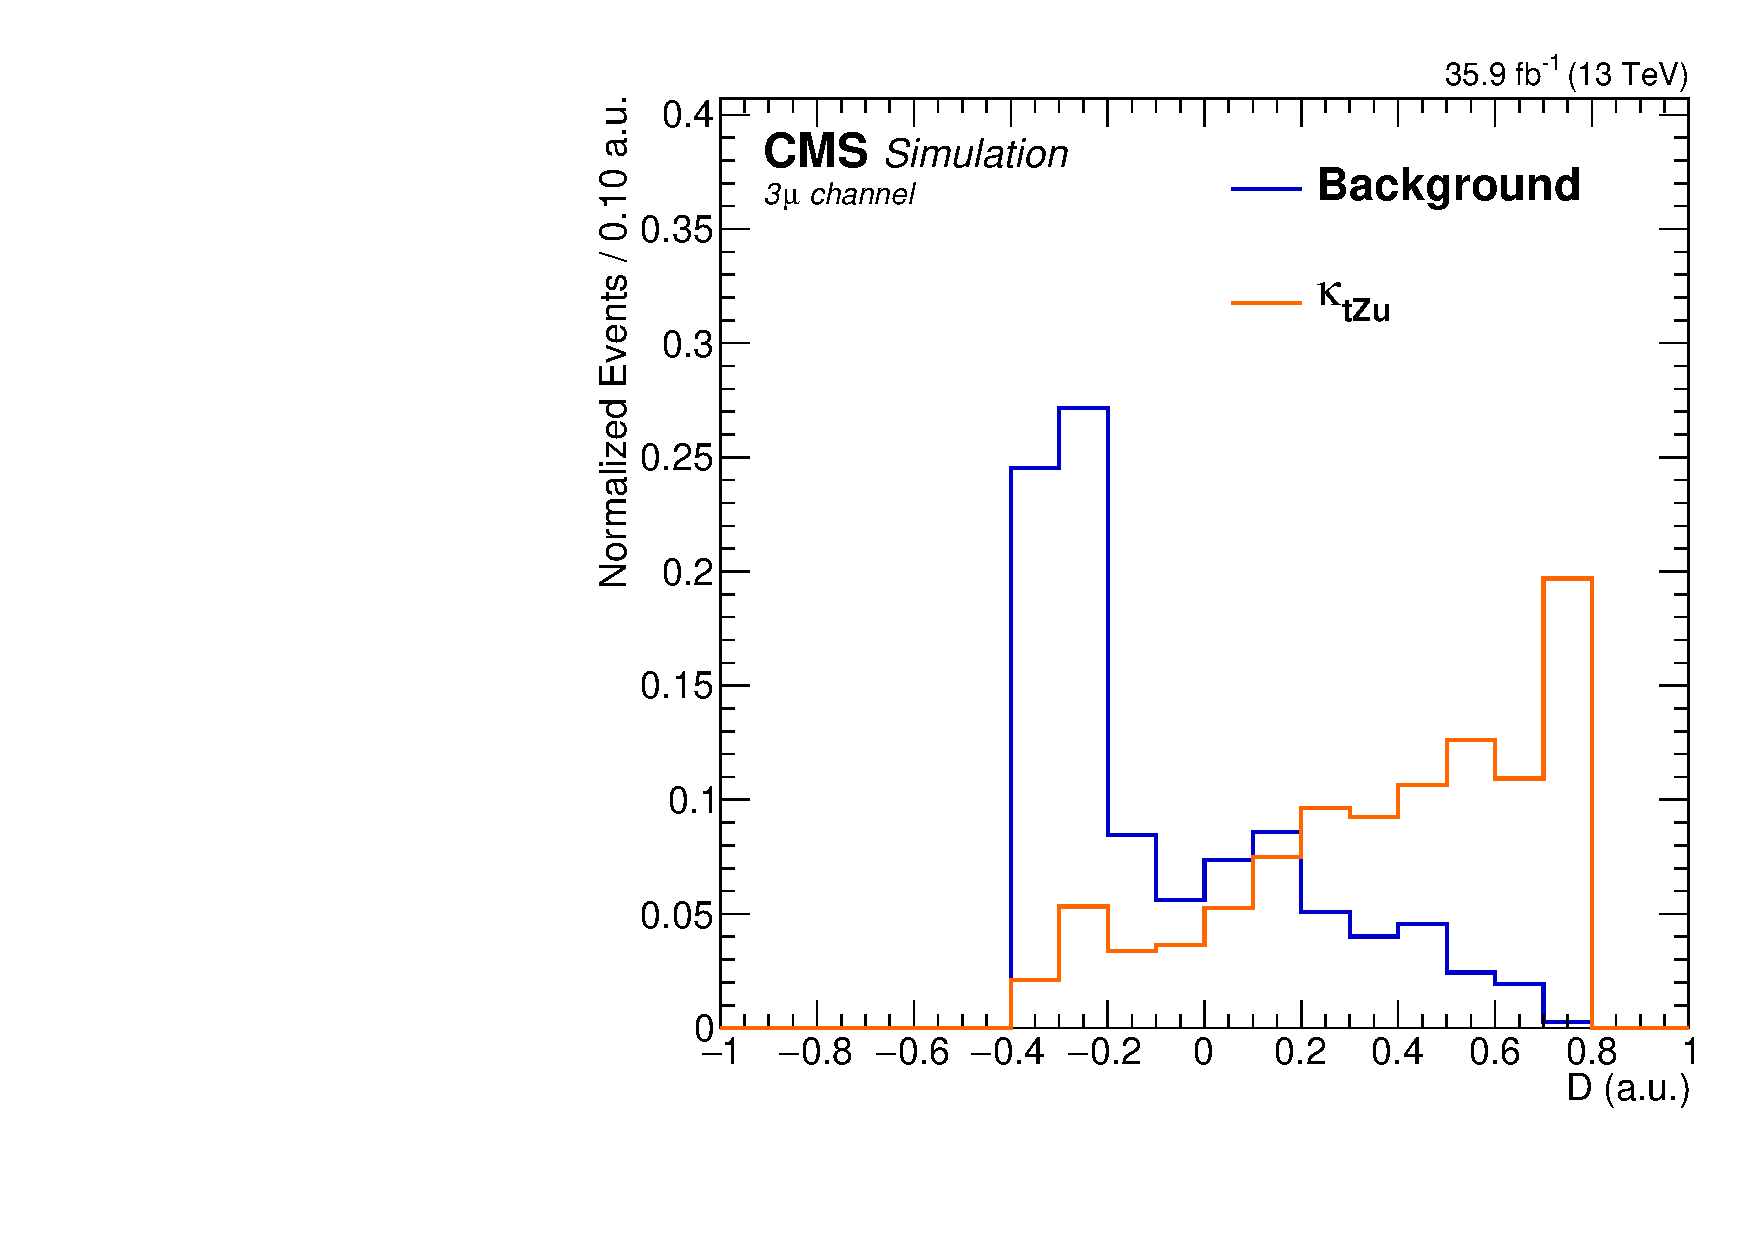
\includegraphics[width=0.24\linewidth]{6_Search/Figures/BDTdistributionsNorm/singletop_Zut_BDT_uuu_Normalized}
%	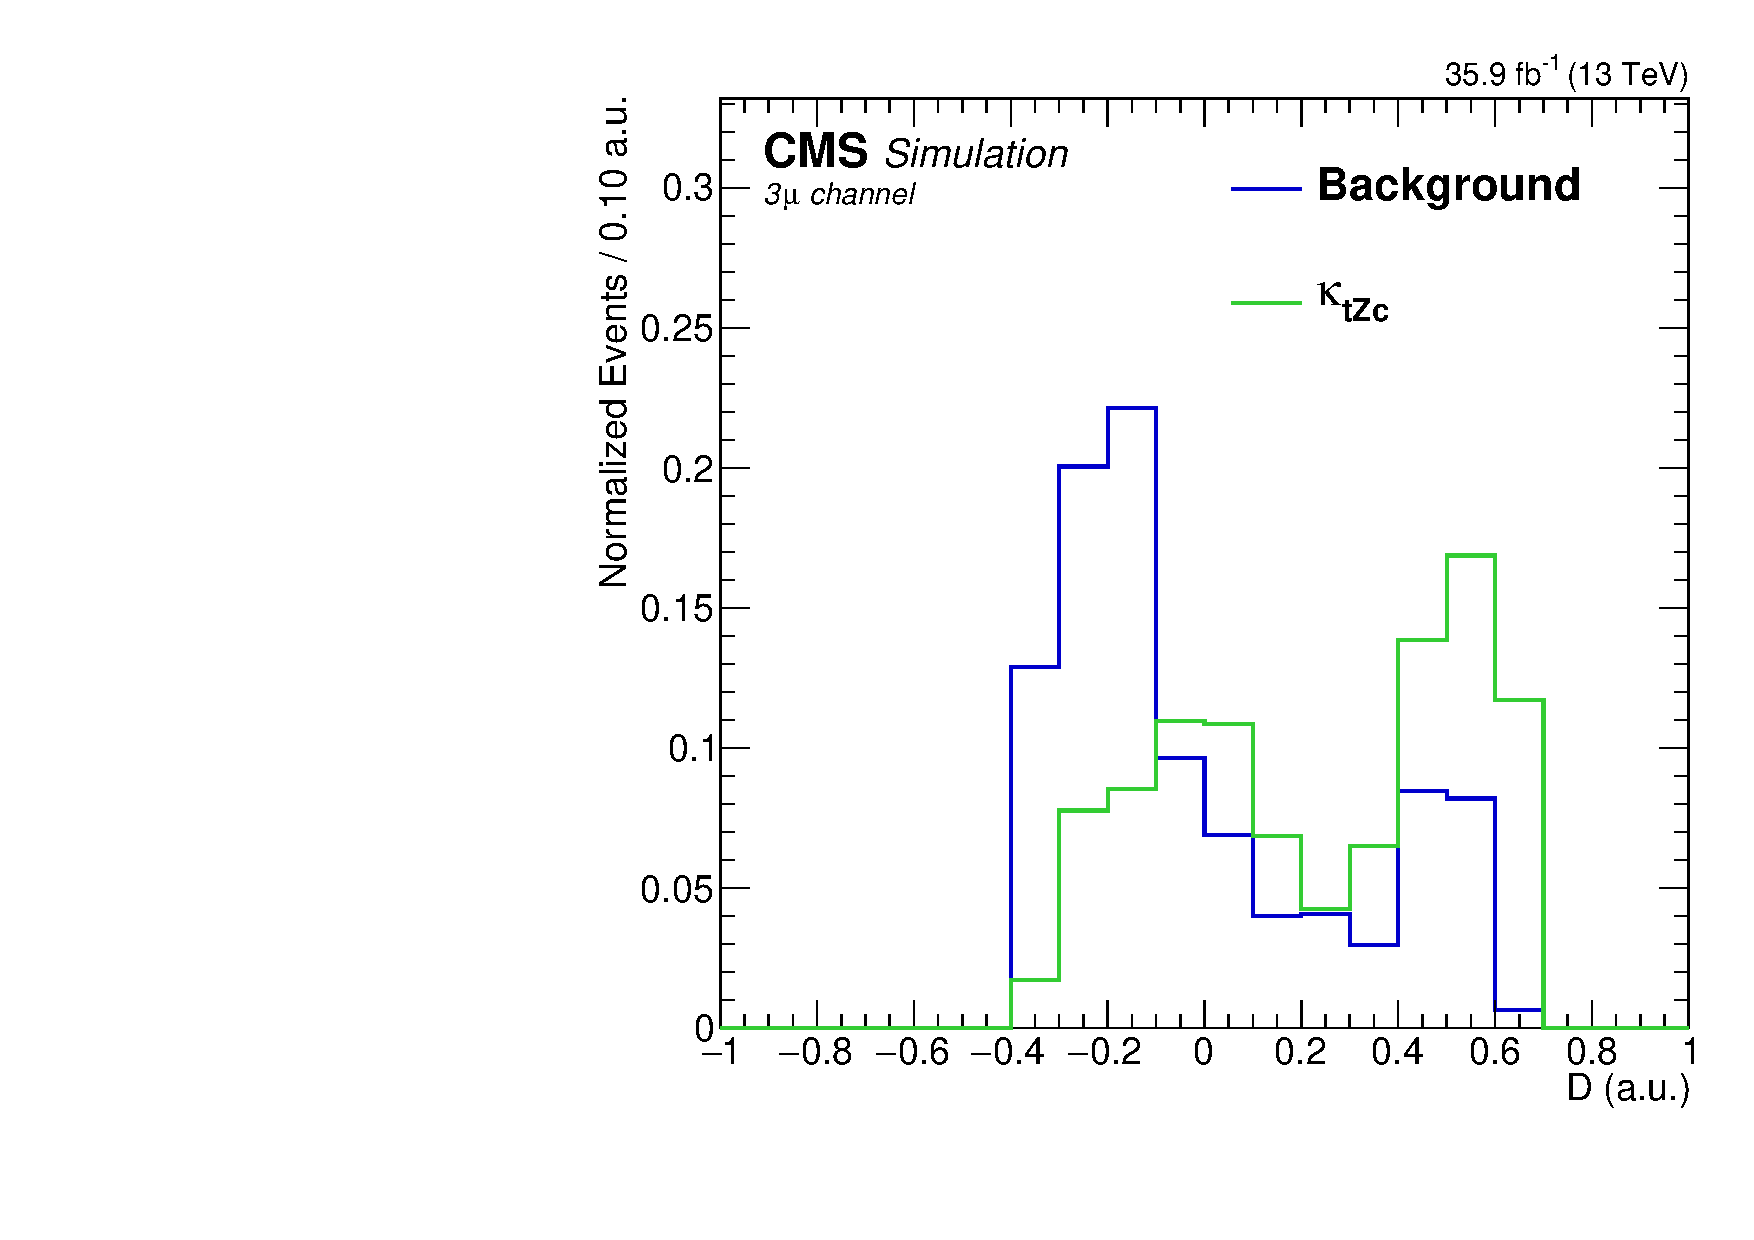
\includegraphics[width=0.24\linewidth]{6_Search/Figures/BDTdistributionsNorm/singletop_Zct_BDT_uuu_Normalized}
%	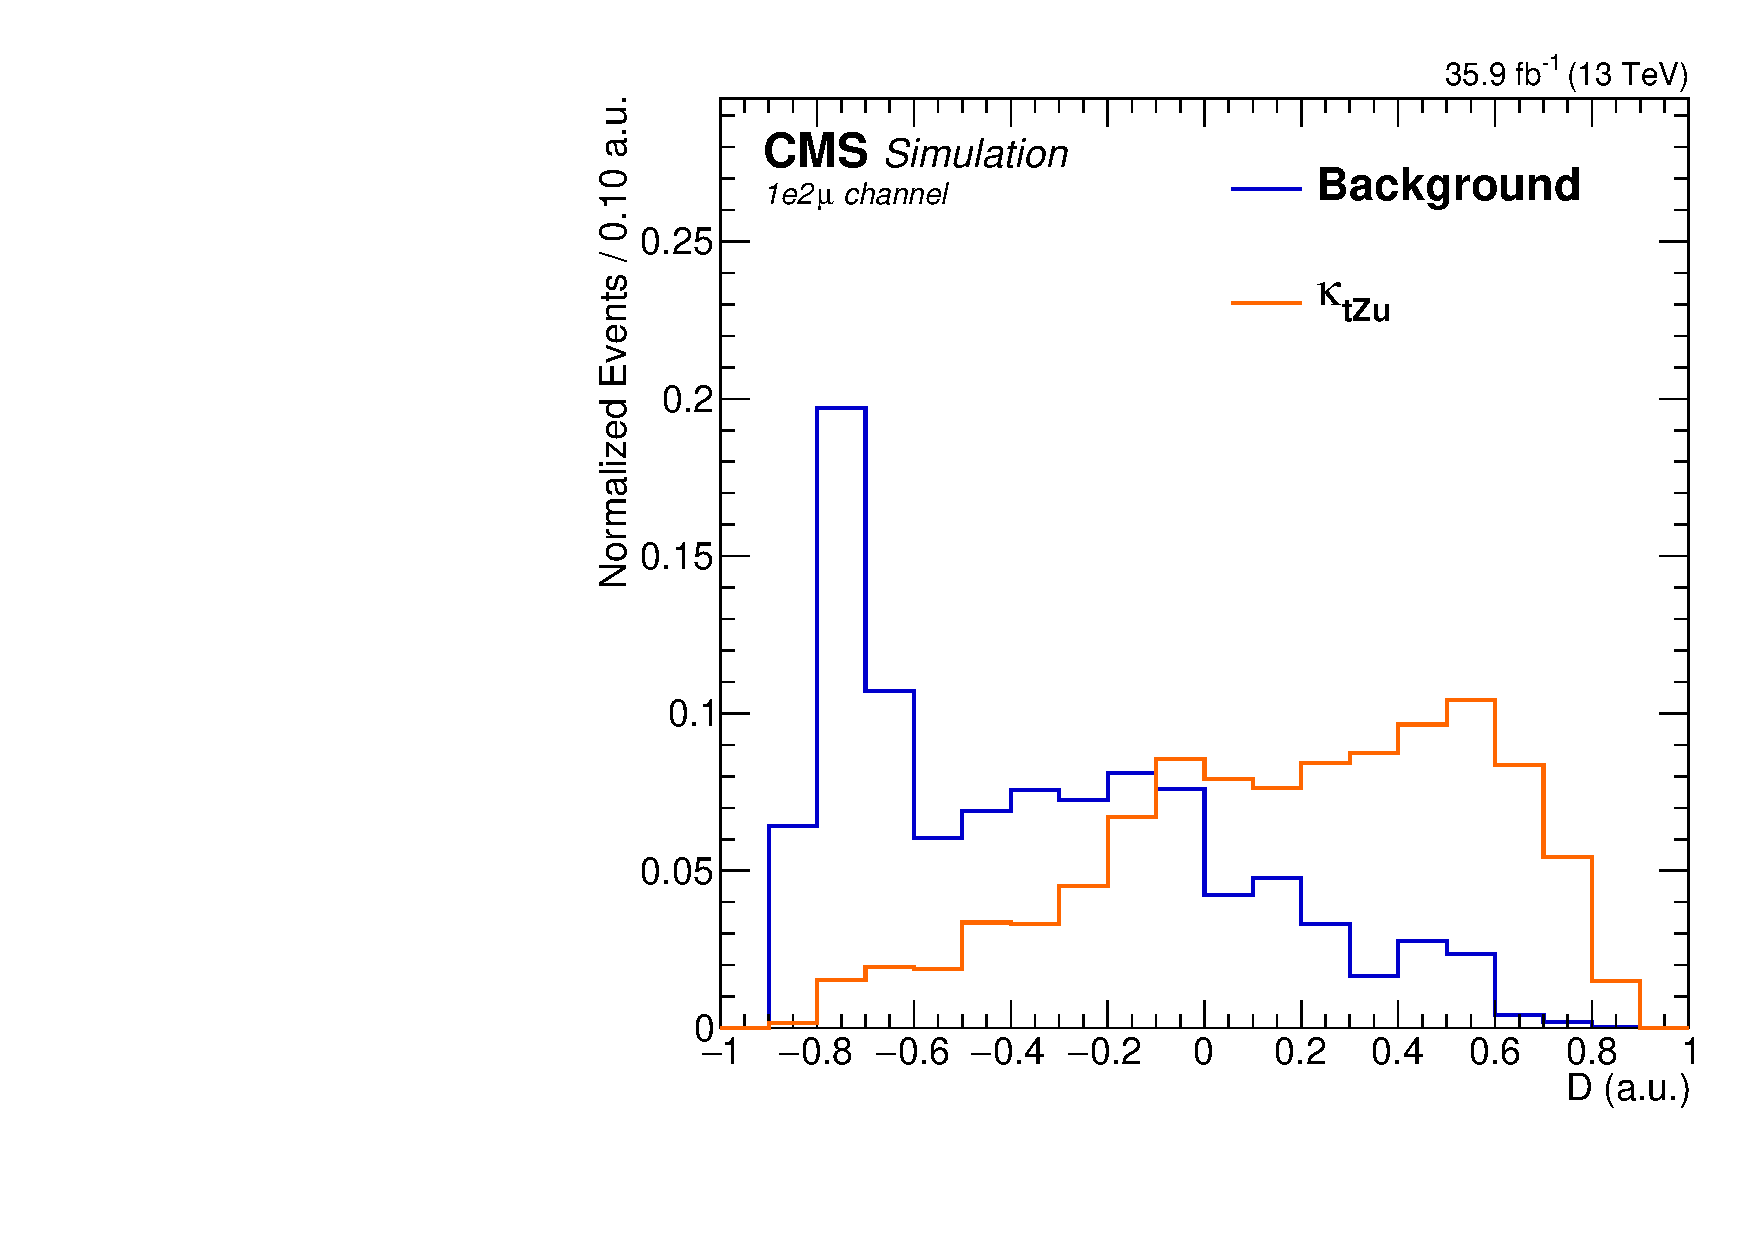
\includegraphics[width=0.24\linewidth]{6_Search/Figures/BDTdistributionsNorm/toppair_Zut_BDT_uue_Normalized}
%	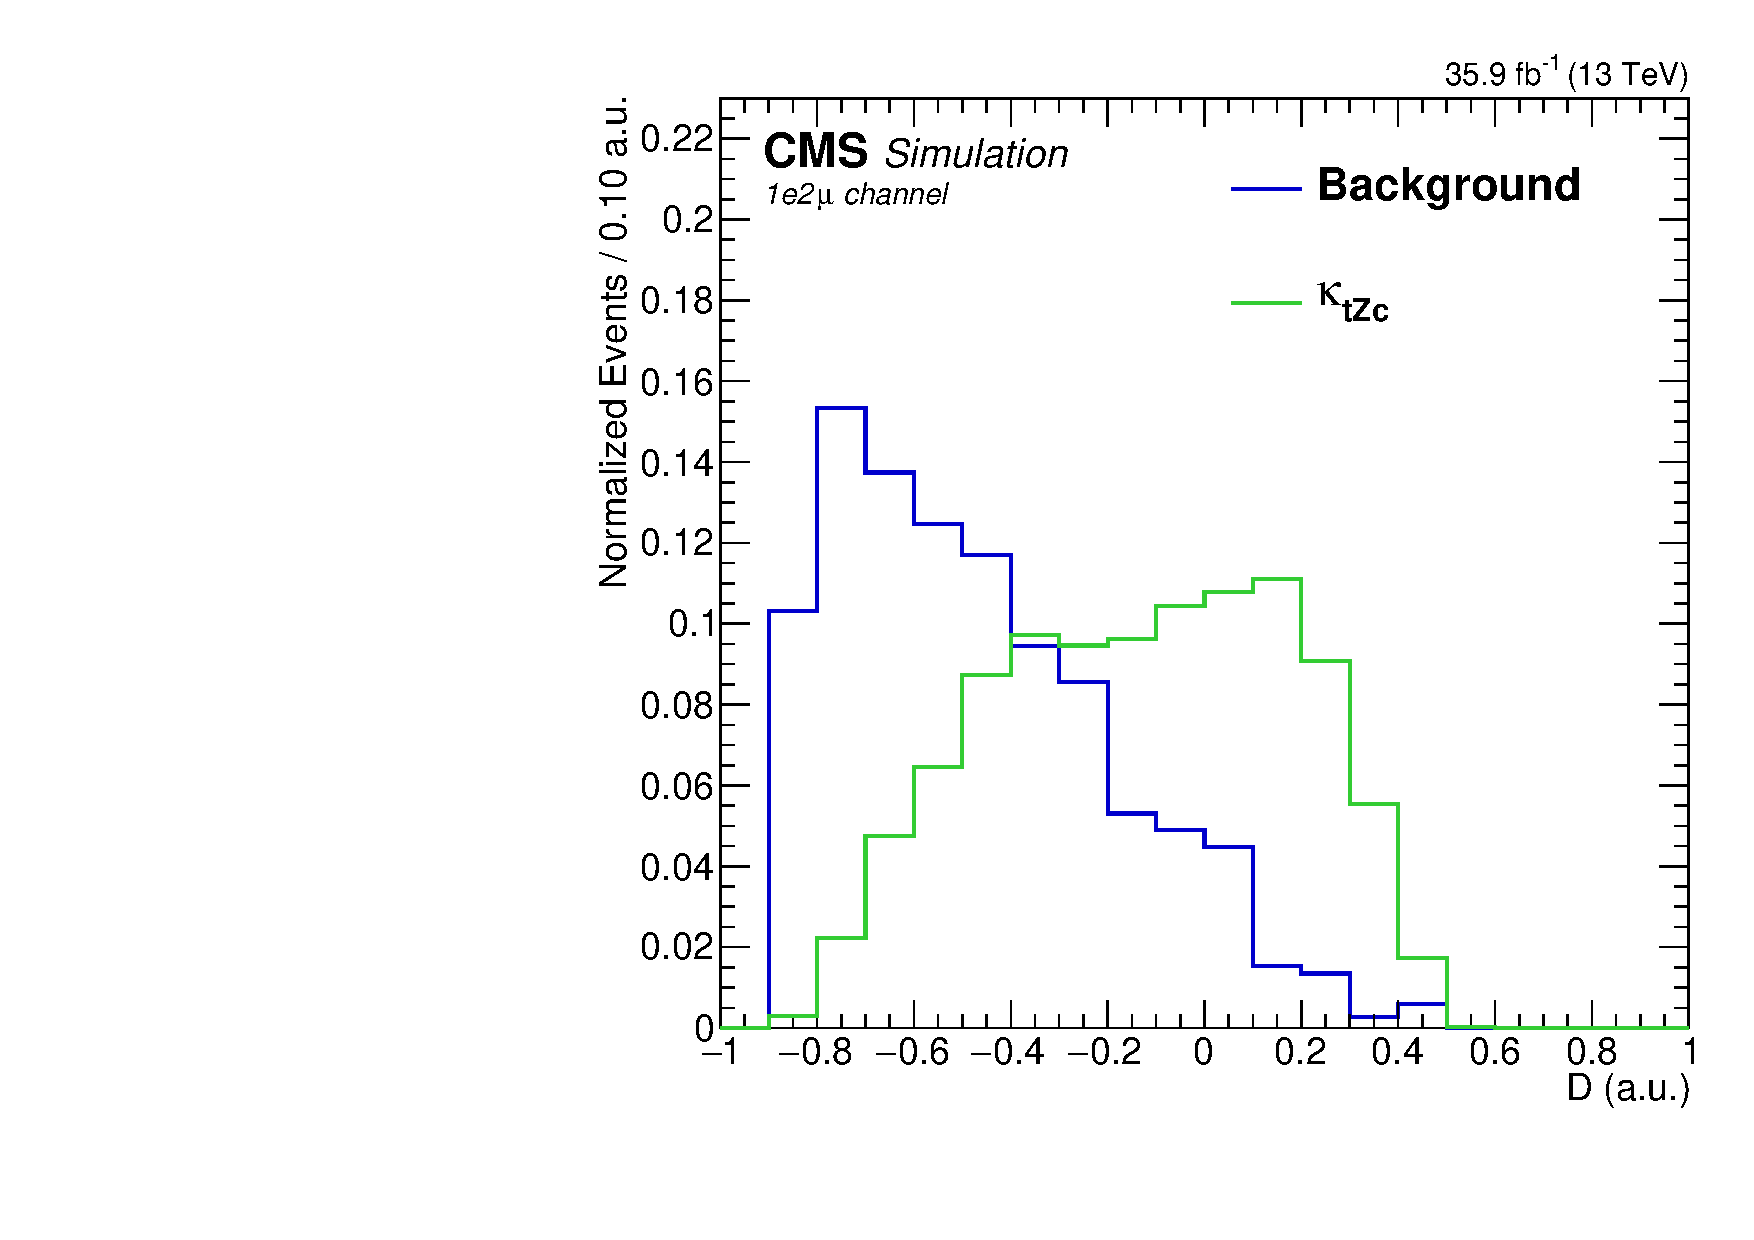
\includegraphics[width=0.24\linewidth]{6_Search/Figures/BDTdistributionsNorm/toppair_Zct_BDT_uue_Normalized}
%	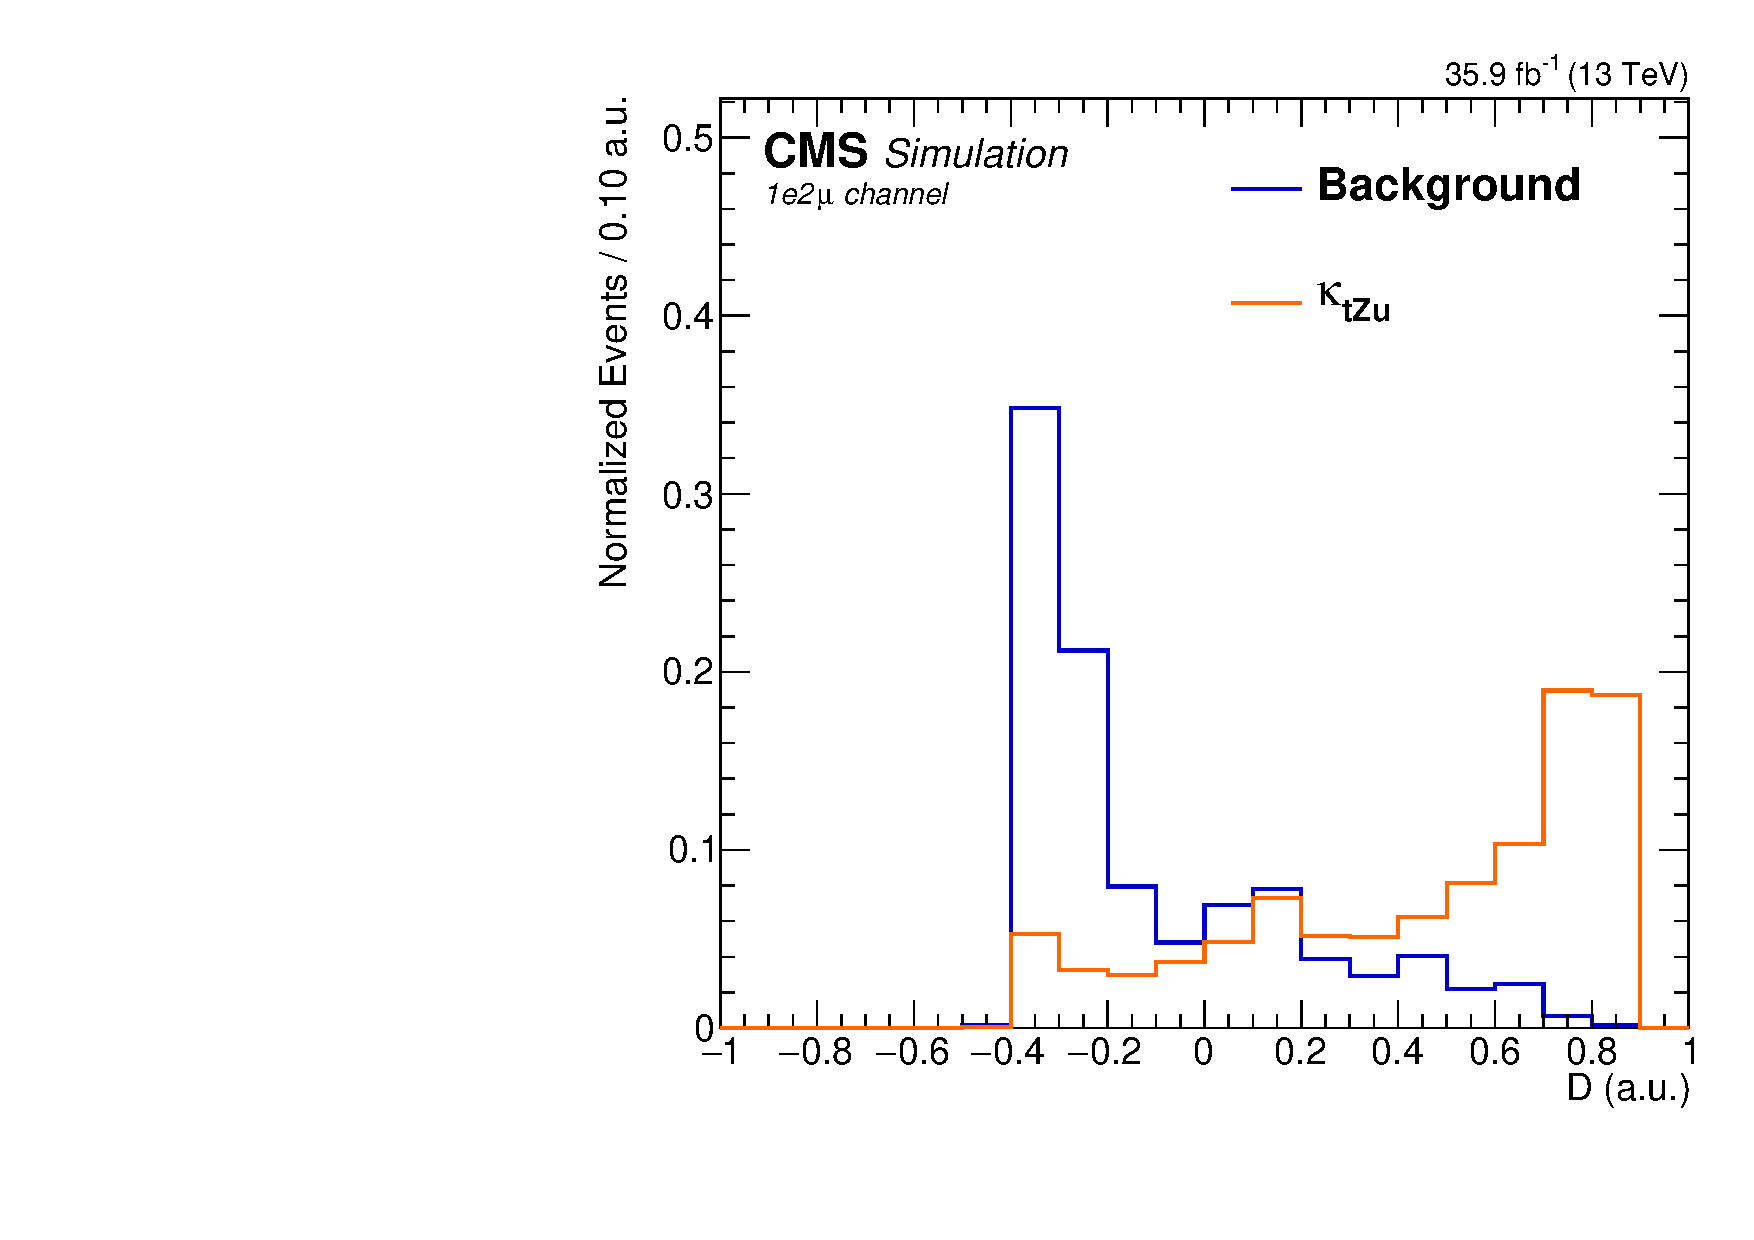
\includegraphics[width=0.24\linewidth]{6_Search/Figures/BDTdistributionsNorm/singletop_Zut_BDT_uue_Normalized}
%	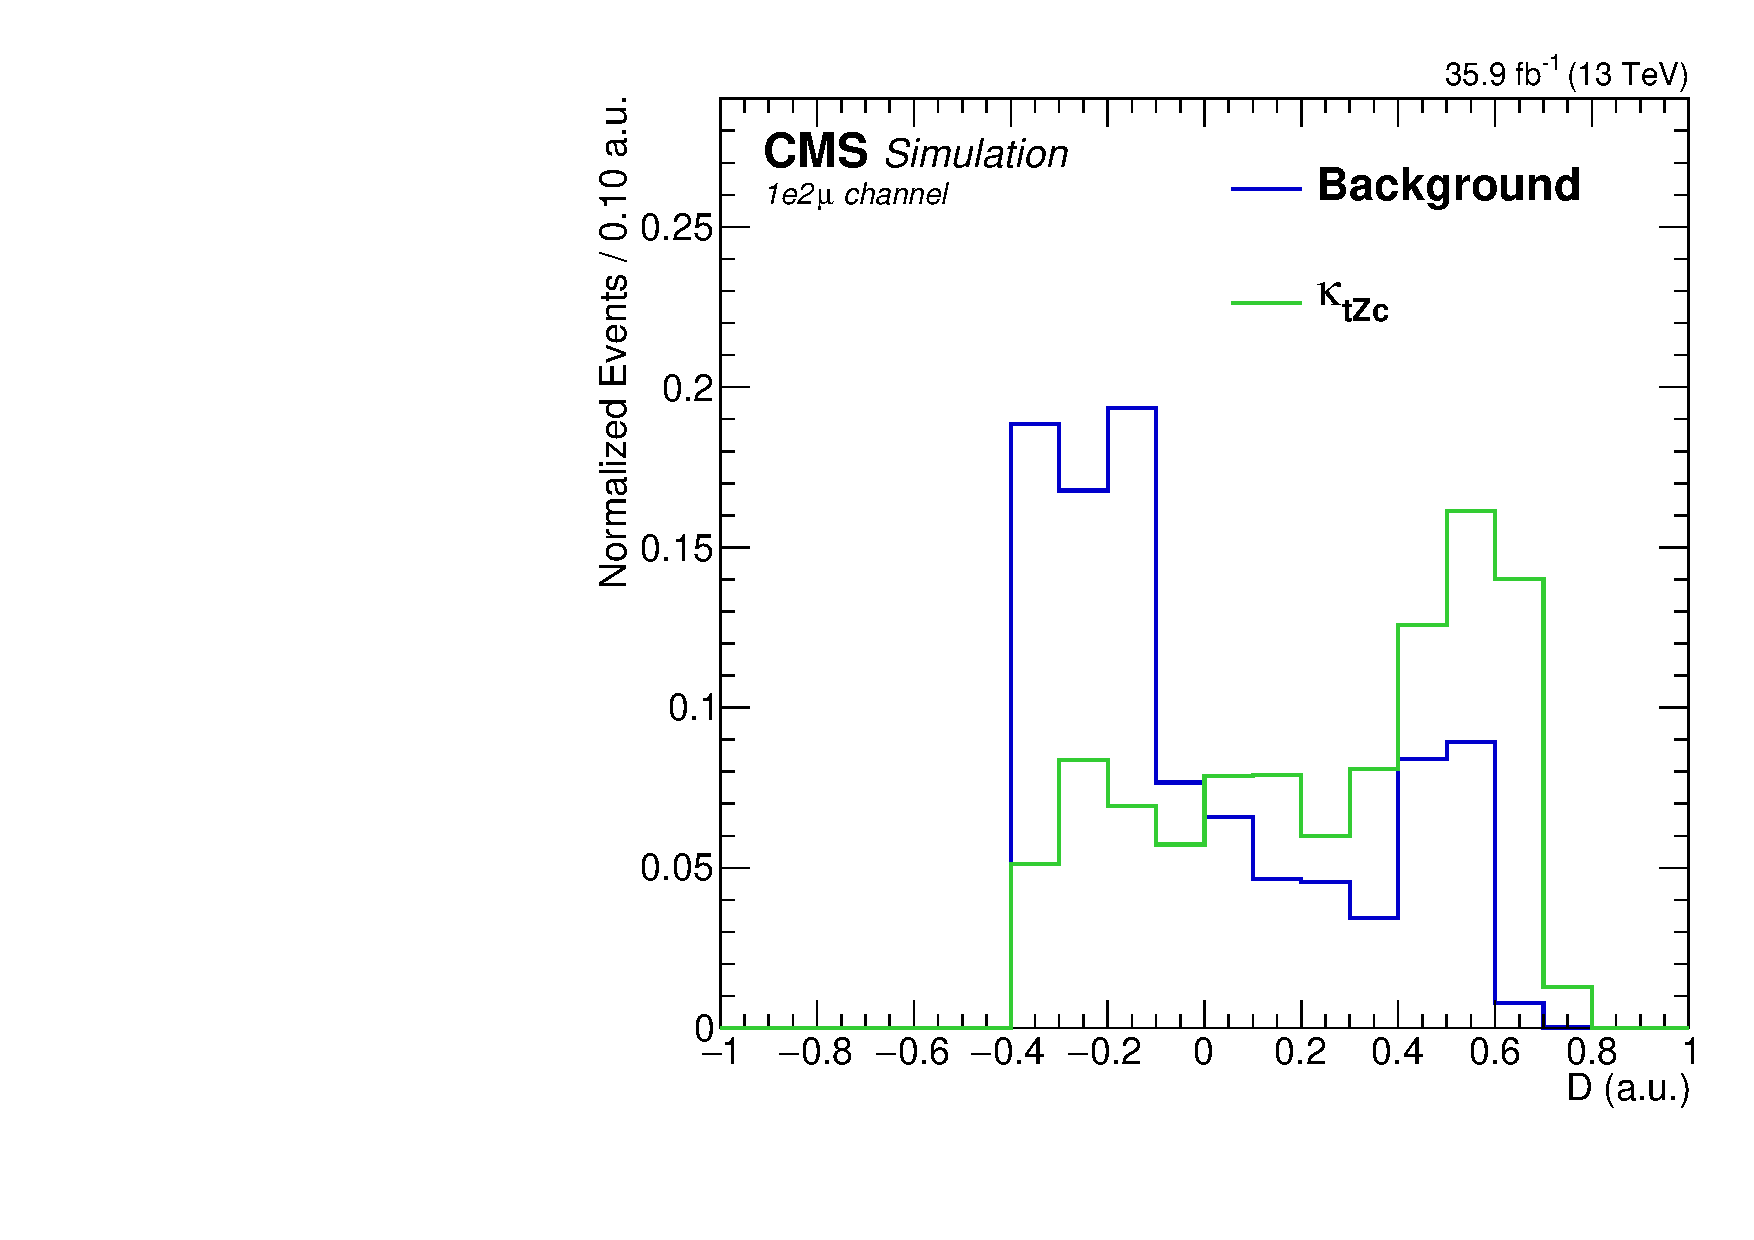
\includegraphics[width=0.24\linewidth]{6_Search/Figures/BDTdistributionsNorm/singletop_Zct_BDT_uue_Normalized}
%	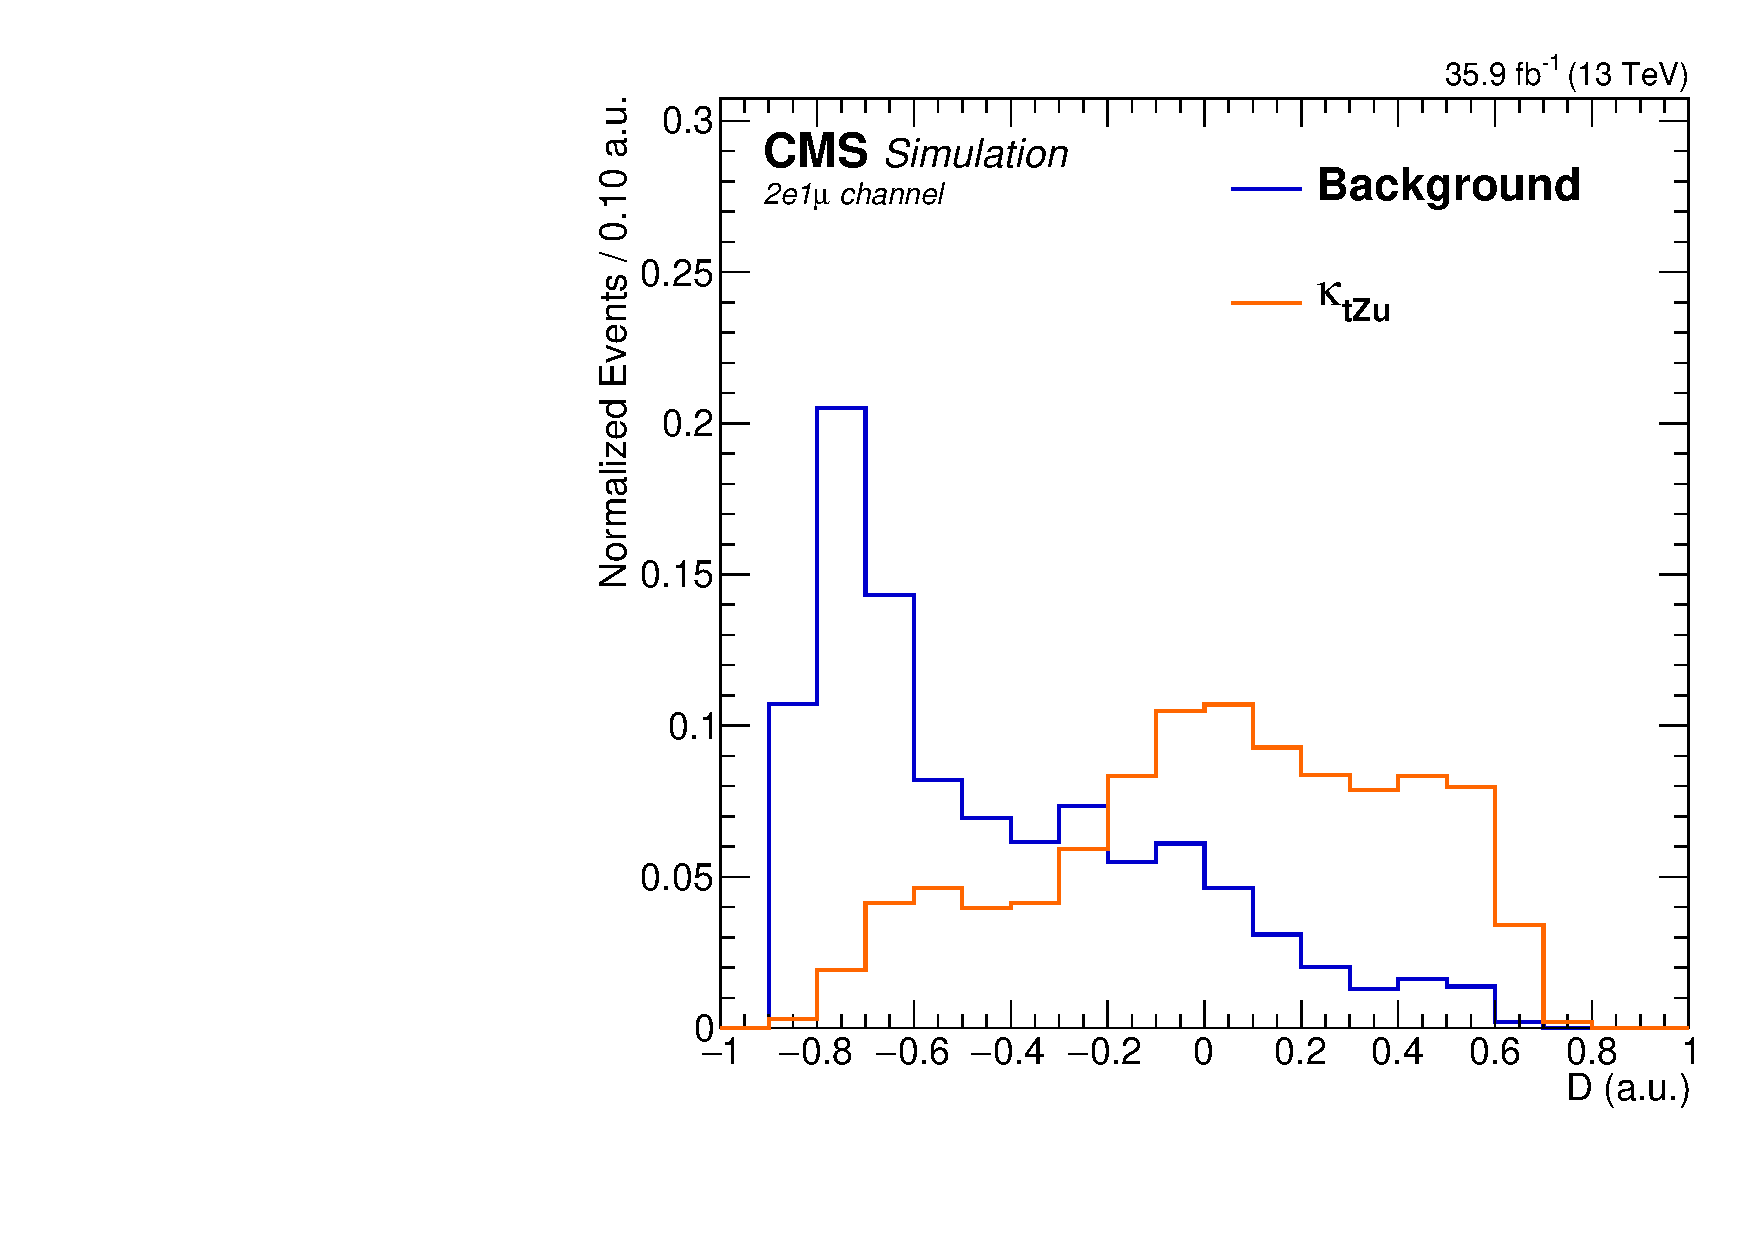
\includegraphics[width=0.24\linewidth]{6_Search/Figures/BDTdistributionsNorm/toppair_Zut_BDT_eeu_Normalized}
%	\includegraphics[width=0.24\linewidth]{6_Search/Figures/BDTdistributionsNorm/toppair_Zct_BDT_eeu_Normalized}
%	\includegraphics[width=0.24\linewidth]{6_Search/Figures/BDTdistributionsNorm/singletop_Zut_BDT_eeu_Normalized}
%	\includegraphics[width=0.24\linewidth]{6_Search/Figures/BDTdistributionsNorm/singletop_Zct_BDT_eeu_Normalized}
%		\includegraphics[width=0.24\linewidth]{6_Search/Figures/BDTdistributionsNorm/toppair_Zut_BDT_eee_Normalized}
%	\includegraphics[width=0.24\linewidth]{6_Search/Figures/BDTdistributionsNorm/toppair_Zct_BDT_eee_Normalized}
%	\includegraphics[width=0.24\linewidth]{6_Search/Figures/BDTdistributionsNorm/singletop_Zut_BDT_eee_Normalized}
%	\includegraphics[width=0.24\linewidth]{6_Search/Figures/BDTdistributionsNorm/singletop_Zct_BDT_eee_Normalized}
%	
%	\caption{Normalised distributions of the discriminating variable before the fit. Each row contains: left: \TTSR\ \Zut , left-middle: \TTSR\ \Zct ; right-middle: \STSR\  \Zut , right: \STSR\  \Zct.  First row: \mumumu\ lepton channel, second row: \emumu, third row: \eemu, and last row: \eee\ lepton channel.}
%	\label{fig:bdtuuunorm}
%\end{figure}	
%	
	

\clearpage
\subsection{Transverse mass in \WZCR}
The \WZCR\ is used to estimate the contribution from \WZ+jets and \NPL\ background. In this region, a fit is performed on the transverse mass distribution of the \PW\ boson. The prefit normalised templates are given in this section. \todo{beschrijf plotjes}
\begin{figure}[htbp]
	\centering
	\includegraphics[width=0.49\linewidth]{6_Search/Figures/MTWnormalised/MTW_uuu_Normalized}
	\includegraphics[width=0.49\linewidth]{6_Search/Figures/MTWnormalised/MTW_uue_Normalized}
	\includegraphics[width=0.49\linewidth]{6_Search/Figures/MTWnormalised/MTW_eeu_Normalized}
	\includegraphics[width=0.49\linewidth]{6_Search/Figures/MTWnormalised/MTW_eee_Normalized}
	\caption{The normalised distribution of the transverse mass of the W boson in the \WZCR, before the fit. Left: \mumumu, left-middle: \emumu, right-middle: \eemu, and right: \eee\ lepton channel.  }
	\label{fig:mtwnorm}
\end{figure}
\begin{figure}[htbp]
	\centering
	\includegraphics[width=0.49\linewidth]{6_Search/Figures/MTWnormalised/MTW_all_Normalized}
	\caption{The normalised distribution of the transverse mass of the W boson in the \WZCR, before the fit. All different lepton channels together. }
	\label{fig:mtwallnorm}
\end{figure}


\section{Systematic uncertainties}
The systematic uncertainties entering the analysis are coming from different sources. The experimental uncertainties arise from the reconstruction of the objects and are discussed in \Sec{sec:PhysicsObject}. These influence the number of events passing the selection, so-called normalisation uncertainties, or the relative occupancies of the distributions, so-called shape
 uncertainties. The normalisation uncertainties coming from reconstruction include the uncertainty of 2.5\% on the measured integrated luminosity and the efficiency of the trigger logic used for the analysis which has a 1\% (5\%) uncertainty on the 
 \mumumu\ and \emumu\ (\eemu\ and \eee) channels. The  pileup distribution is calculated via the minimum bias cross section which has a 4.6\% uncertainty. This uncertainty results in a systematic shift in the pileup distribution and its shape effect is estimated by recalculating the pileup distribution for each variation of the minimum bias cross section. The shape uncertainties also include the uncertainties coming from the applied lepton scale factors. Their systematic uncertainty originates from three sources: identification, isolation and tracking.  The uncertainties arising from jet energy corrections require a recalculation of all jet related kinematic observables and its effect is propagated to the missing transverse energy.  The reweighting of the CSVv2 discriminant is also a source of uncertainty. There are three sources of uncertainty contributing to the measurement of the b-tag related scale factors: statistical uncertainties, jet energy scale and the purity of the sample. These result in eight uncorrelated contributions. 
 
 Since the \NPL\ sample is artificially made from data by inverting the isolation of the third lepton. Its effect has to be estimated. The shape uncertainty one the \NPL\ processes is obtained by varying the isolation inversion with respect to tight working point to the loose working point for electrons and muons at the same time. This found to have negligible effect. The uncertainty on the normalisation of the overall \NPL\ yield is taken as 50\% in accordance with the \SM\ \tZq\ search~\cite{CMS-PAS-TOP-16-020}.
 
 The uncertainty on the expected yield of the simulated backgrounds is taken to be 30\% of the yield such that it covers all uncertainties at next to leading order accuracy. Theory uncertainties  originating from the modelling of the main backgrounds are estimated to account for the effect on the shape of the distributions from the choice of parton density funnctions, and renormalization (\muR) and factorization (\muF) scales. The effect of the  renormalization (\muR) and factorization (\muF) scales is estimated by varying each independently and correlated up and down by a factor of two, where the anti-correlated variations are dropped. The envelope of these variations is used as an uncertainty. The uncertainties coming from the parton density functions  used for simulation are estimated using the PDF4LHC recipe~\cite{Ball:2017nwa}, which combines the MMHT14, CT14, and NNPDF3.0 PDF sets~\cite{Ball:2017nwa}. The theory uncertainties are considered for the main backgrounds coming from simulation: \WZ+jets, \ZZ+jets, \ttZ, and \tZq. This is found to have a negligible effect.

 The way the uncertainties are treated as nuisance parameters is summarized in \tab{tab:nuis}. The effect of systematic uncertainties that are treated as shape uncertainties is shown in \Sec{sec:MTW} and \Sec{sec:BDTsys} . \todo{INCLUDE EFFECT PDF AND FACT/RENO}

\begin{table}[htbp]
	\centering
	\caption{Uncertainties used in this analysis. The column labelled type represents how the uncertainty is treated for the fit.}
	\begin{tabular}{ccc}
		\toprule
		Source & Systematic input & Type \\ 
		\midrule 
		nonprompt muon norm. & 50\% & normalisation \\ 
		 
		nonprompt electron norm. & 50\% & normalisation \\ 
		 
		background \ttZ\ norm. & 30\% & normalisation \\ 
		 
		background \WZ\ norm. & 30\% & normalisation \\ 
		 
		background \tZq\ norm. & 30\% & normalisation \\ 
		 
		background \ZZ\ norm.& 30\% & normalisation \\ 
		 
		background other MC norm. & 30\% & normalisation \\ 
		 
		trigger & 1\% (5\%) & normalisation \\ 
		 
		lepton identification  & $\pm \sigma(p_{T},\eta)$ & shape \\ 
		 
		JES & $\pm \sigma(p_{T},\eta)$ & shape \\ 
		 
		JER & $\pm \sigma(p_{T},\eta)$ &  shape \\ 
		 
		b-tagging & $\pm \sigma(p_{T},\eta)$ & shape \\ 
		 
		pileup\ & $\pm \sigma$ of min. bias cross section &  shape \\ 
		 
		PDF & PDF4LHC recipe &  shape   \\ 
		 
		luminosity & 2.5\% & normalisation \\ 
		 
		renorm. and fact. scales & varying indep. and corr. &  shape \\ 
		\bottomrule
	\end{tabular} 
	\label{tab:nuis}
\end{table}
\clearpage
\subsection{Effect of systematic uncertainties on the transverse mass distribution}
\label{sec:MTW}
\begin{figure}[htbp] 
	\centering 
	\subbottom[Pileup uncertainty]{
	    \includegraphics[width=0.2\linewidth]{6_Search/Figures/SystematicEffect/MTWsys/MWT_pileupBKG}
    }
    \subbottom[Electron identification  uncertainty]{
    	\includegraphics[width=0.2\linewidth]{6_Search/Figures/SystematicEffect/MTWsys/MWT_electronBKG}
    }
    \subbottom[Muon identification uncertainty]{
    	\includegraphics[width=0.2\linewidth]{6_Search/Figures/SystematicEffect/MTWsys/MWT_muonBKG}
    }
	\subbottom[Jet energy scale uncertainty]{
		\includegraphics[width=0.2\linewidth]{6_Search/Figures/SystematicEffect/MTWsys/MTW_JESBKG}
	}
	\subbottom[Jet energy resolution uncertainty]{
		\includegraphics[width=0.2\linewidth]{6_Search/Figures/SystematicEffect/MTWsys/MTW_JERBKG}
	}
	\subbottom[CSVv2: cf uncertainty~(1)]{
		\includegraphics[width=0.2\linewidth]{6_Search/Figures/SystematicEffect/MTWsys/MWT_btagSF_cferr1BKG}
	}
    \subbottom[CSVv2: cf uncertainty~(2)]{
    	\includegraphics[width=0.2\linewidth]{6_Search/Figures/SystematicEffect/MTWsys/MWT_btagSF_cferr2BKG}
    }
    \subbottom[CSVv2: hf uncertainty]{
     	\includegraphics[width=0.2\linewidth]{6_Search/Figures/SystematicEffect/MTWsys/MWT_btagSF_hfBKG}
    }
    \subbottom[CSVv2: lf uncertainty ]{
    	\includegraphics[width=0.2\linewidth]{6_Search/Figures/SystematicEffect/MTWsys/MWT_btagSF_lfBKG}
    }
    \subbottom[CSVv2: hf statistical uncertainty~(1) ]{
    	\includegraphics[width=0.2\linewidth]{6_Search/Figures/SystematicEffect/MTWsys/MWT_btagSF_hfstats1BKG}
    }
    \subbottom[CSVv2: hf statistical uncertainty~(2) ]{
		\includegraphics[width=0.2\linewidth]{6_Search/Figures/SystematicEffect/MTWsys/MWT_btagSF_hfstats2BKG}
    }
    \subbottom[CSVv2: lf statistical uncertainty~(1) ]{
    	\includegraphics[width=0.2\linewidth]{6_Search/Figures/SystematicEffect/MTWsys/MWT_btagSF_lfstats1BKG}
    }
    \subbottom[CSVv2: lf statistical uncertainty~(2) ]{
		\includegraphics[width=0.2\linewidth]{6_Search/Figures/SystematicEffect/MTWsys/MWT_btagSF_lfstats2BKG}
	}
\subbottom[Factorisation and renormalization scale uncertainty ]{
	\includegraphics[width=0.2\linewidth]{6_Search/Figures/theorysys/factrenoall}
}
\subbottom[PDF uncertainty ]{
	\includegraphics[width=0.2\linewidth]{6_Search/Figures/theorysys/pdfbdtall}
}
	\caption{Distribution of the nominal values and shift due to  systematic uncertainties for the transverse mass of the \PW\ boson in the \WZCR\ for the \WZ\ process. All lepton channels summed.}
	\label{fig:shiftMTW}
\end{figure}
\newpage
\subsection{Effect of the systematic uncertainties on the multivariate discriminator distributions}
\label{sec:BDTsys}
The  effect of the systematic uncertainties on the multivariate discriminator in the \STSR\ involving the \Zut\ vertex is shown. Other regions are shown in \App{app:sys}. \todo{Bespreek plotjes}

 %./BDTAnalyzer Ntup MVAinput/BDT_toppair_Zct/Reader_BDT_toppair_Zct_MVA_regionEq1.root Zct  toppair  PlotJeSystematics doSystematics

\begin{figure}[htbp] 
	\centering 
	\subbottom[Pileup uncertainty]{
		\includegraphics[width=0.2\linewidth]{6_Search/Figures/SystematicEffect/singletopzut/pileupBKG}
		\includegraphics[width=0.2\linewidth]{6_Search/Figures/SystematicEffect/singletopzut/pileupSIG}
	}
	\subbottom[Electron identification  uncertainty]{
		\includegraphics[width=0.2\linewidth]{6_Search/Figures/SystematicEffect/singletopzut/electronBKG}
		\includegraphics[width=0.2\linewidth]{6_Search/Figures/SystematicEffect/singletopzut/electronSIG}
	}
	\subbottom[Muon identification uncertainty]{
		\includegraphics[width=0.2\linewidth]{6_Search/Figures/SystematicEffect/singletopzut/muonBKG}
		\includegraphics[width=0.2\linewidth]{6_Search/Figures/SystematicEffect/singletopzut/muonSIG}
	}
	\subbottom[Jet energy scale uncertainty]{
		\includegraphics[width=0.2\linewidth]{6_Search/Figures/SystematicEffect/singletopzut/JESBKG}
		\includegraphics[width=0.2\linewidth]{6_Search/Figures/SystematicEffect/singletopzut/JESSIG}
	}
	\subbottom[Jet energy resolution uncertainty]{
		\includegraphics[width=0.2\linewidth]{6_Search/Figures/SystematicEffect/singletopzut/JERBKG}
		\includegraphics[width=0.2\linewidth]{6_Search/Figures/SystematicEffect/singletopzut/JERSIG}
	}
\subbottom[Factorisation and renormalization scale normalised uncertainty ]{
	\includegraphics[width=0.22\linewidth]{6_Search/Figures/theorysys/factrenosinglezutbdtall}
}
\subbottom[PDF normalised uncertainty ]{
	\includegraphics[width=0.22\linewidth]{6_Search/Figures/theorysys/pdfsinglezutbdtall}
}

	\caption{Distribution of the nominal values and shift due to systematic uncertainties for the transverse mass of the \PW\ boson in the \STSR\ for the \WZ\ process and FCNC signal involving a \Zut\ vertex. All lepton channels summed. Part one.}
\label{fig:shiftBDTSTZut1}
\end{figure}
\begin{figure}[htbp] 
	\centering 
	\subbottom[CSVv2: cf uncertainty~(1)]{
		\includegraphics[width=0.2\linewidth]{6_Search/Figures/SystematicEffect/singletopzut/btagSF_cferr1BKG}
		\includegraphics[width=0.2\linewidth]{6_Search/Figures/SystematicEffect/singletopzut/btagSF_cferr1SIG}
	}
	\subbottom[CSVv2: cf uncertainty~(2)]{
		\includegraphics[width=0.2\linewidth]{6_Search/Figures/SystematicEffect/singletopzut/btagSF_cferr2BKG}
		\includegraphics[width=0.2\linewidth]{6_Search/Figures/SystematicEffect/singletopzut/btagSF_cferr2SIG}
	}
	\subbottom[CSVv2: hf uncertainty]{
		\includegraphics[width=0.2\linewidth]{6_Search/Figures/SystematicEffect/singletopzut/btagSF_hfBKG}
		\includegraphics[width=0.2\linewidth]{6_Search/Figures/SystematicEffect/singletopzut/btagSF_hfSIG}
	}
	\subbottom[CSVv2: lf uncertainty ]{
		\includegraphics[width=0.2\linewidth]{6_Search/Figures/SystematicEffect/singletopzut/btagSF_lfBKG}
		\includegraphics[width=0.2\linewidth]{6_Search/Figures/SystematicEffect/singletopzut/btagSF_lfSIG}
	}
	\subbottom[CSVv2: hf statistical uncertainty~(1) ]{
		\includegraphics[width=0.2\linewidth]{6_Search/Figures/SystematicEffect/singletopzut/btagSF_hfstats1BKG}
		\includegraphics[width=0.2\linewidth]{6_Search/Figures/SystematicEffect/singletopzut/btagSF_hfstats1SIG}
	}
	\subbottom[CSVv2: hf statistical uncertainty~(2) ]{
		\includegraphics[width=0.2\linewidth]{6_Search/Figures/SystematicEffect/singletopzut/btagSF_hfstats2BKG}
		\includegraphics[width=0.2\linewidth]{6_Search/Figures/SystematicEffect/singletopzut/btagSF_hfstats2SIG}
	}
	\subbottom[CSVv2: lf statistical uncertainty~(1) ]{
		\includegraphics[width=0.2\linewidth]{6_Search/Figures/SystematicEffect/singletopzut/btagSF_lfstats1BKG}
		\includegraphics[width=0.2\linewidth]{6_Search/Figures/SystematicEffect/singletopzut/btagSF_lfstats1SIG}
	}
	\subbottom[CSVv2: lf statistical uncertainty~(2) ]{
		\includegraphics[width=0.2\linewidth]{6_Search/Figures/SystematicEffect/singletopzut/btagSF_lfstats2BKG}
		\includegraphics[width=0.2\linewidth]{6_Search/Figures/SystematicEffect/singletopzut/btagSF_lfstats2SIG}
	}
	\caption{Distribution of the nominal values and shift due to systematic uncertainties for the transverse mass of the \PW\ boson in the \STSR\ for the \WZ\ process and FCNC signal involving a \Zut\ vertex. All lepton channels summed. Part two.}
	\label{fig:shiftBDTSTZut}
\end{figure}
\clearpage
\section{Limit setting procedure validation}
The analysis strategy has been established using a blinded strategy. Through the use of a pseudo dataset, the limit setting procedure has been validated. Signal injection tests for which the signal strength from a pseudo dataset with a pre-set  signal strength is estimated are performed and shown in \fig{fig:plotzut}. \todo{Bespreek plotjes}
\begin{figure}[htbp]
	\centering
	 \includegraphics[width=0.49\linewidth]{6_Search/Figures/SignalInjection/plotZut}
	 \includegraphics[width=0.49\linewidth]{6_Search/Figures/SignalInjection/plotZct}
	\caption{The  obtained signal strength with the Maximum Likelihood method is in agreement with the signal strength used to generate the Asimov data set for the \Zut\ (left) and \Zct\ (right) couplings.}
	\label{fig:plotzut}
\end{figure}

Another validation has been done by performing a Maximum Likelihood fit in the \WZCR\ only, considering all lepton channels. A simultaneous fit of the signal strength of the \NPE, \NPM\ and the \WZ+jets backgrounds is done by using the multi-dimensional fit in \texttt{Higgs} \texttt{Combine} \texttt{Tool}. The resulting signal strengths can then be applied on the distribution o f the transverse mass of the \PW\ boson to verify data/MC agreement, as can be seen in \fig{fig:mtwstack}. Furthermore, a goodness of fit test is performed, resulting in a p-value of 0.3 (see \fig{fig:gof} ) .

\begin{figure}[htbp]
	\centering
	 \includegraphics[width=0.7\linewidth]{6_Search/Figures/GOF/GOF_1000toys}
	\caption{Goodness of fit testing in the \WZCR\  with 1000 toys. The likelihood ration is denoted as $\lambda$.}
	\label{fig:gof}
\end{figure}

\begin{figure}[htbp]
	\centering
	\includegraphics[width=0.49\linewidth]{6_Search/Figures/InitialFit/vars/wzcontrol_MVA_mWt_uuu_Stack}
	\includegraphics[width=0.49\linewidth]{6_Search/Figures/InitialFit/vars/wzcontrol_MVA_mWt_uue_Stack}
	\includegraphics[width=0.49\linewidth]{6_Search/Figures/InitialFit/vars/wzcontrol_MVA_mWt_eeu_Stack}
	\includegraphics[width=0.49\linewidth]{6_Search/Figures/InitialFit/vars/wzcontrol_MVA_mWt_eee_Stack}
	\caption{The transverse mass of the \PW\ boson in the \WZCR\ for the \mumumu\ channel (left, upper), \emumu\ channel (right, upper), \eemu\ channel (left, lower), and 3 electrons channel (right, lower). The uncertainty band does not include theoretical uncertainties.}
	\label{fig:mtwstack}
\end{figure}


\newpage
\section{Results and discussion}
The limit setting procedure explained in \Sec{sec:Stat} is applied and results are obtained for each lepton channel separately as well as the combination. For both the \Zut\ and \Zct\ coupling, the maximum likelihood estimator of their signal strengths $\hat{\mu}$ is compatible with zero. This is shown in \fig{fig:mlezut}. One can see that the \eee\ lepton channel has the largest uncertainty. This is due to the fact that this channel is the most influences by the lack of statistics for this search.
\begin{figure}[htbp]
	\centering
	\includegraphics[width=0.49\linewidth]{6_Search/Figures/MLE/MLEZut.pdf}
	\includegraphics[width=0.49\linewidth]{6_Search/Figures/MLE/MLEZct.pdf}
	\caption{The maximum likelihood estimators for the signal strengths for the \Zut\ vertex (right) and \Zct\ vertex (left) per lepton channel as well as the combination in the \STSR, \TTSR, and all regions combined. }
	\label{fig:mlezut}
\end{figure}

The maximum likelihood estimators for the nuisance parameters $\hat{\theta}$ are shown in \fig{fig:171102zctmle} for the \Zct\ interaction and in the Appendix (\fig{fig:171102zutmle}) for the \Zut\ interaction. Their values obtained from the signal plus background or background only fits are in agreement. The transfer factors have an initial value different than one and have small uncertainties. The normalisation uncertainties on the yields of the simulated backgrounds get constrained by the fit.  %A well known verification of the error coverage for the fit is the pull distribution. For a random variable $x$ following a Gaussian distribution of mean $m$ and width $w$, the pull $g$ is defined as
%\begin{equation}
% g = \frac{x - m}{w},
%\end{equation}
%and follows a standard Gaussian with mean zero and unit width. This property can be applied to our case of parameter estimation due to the central limit theorem~\cite{CDF:AN5776}. The pull distributions are shown in \fig{fig:pulls}. These are peaking at zero with tails going to $\pm2.5$.
%\begin{figure}[htbp]
%	\centering
%	\includegraphics[width=.49\linewidth]{6_Search/Figures/impact/pullsZutwithMC.pdf}
%	\includegraphics[width=.49\linewidth]{6_Search/Figures/impact/pullsZctwithMC.pdf}
%	\caption{Post-fit distribution of the pulls for the \Zut\ (left) and \Zct\ (right) vertex.}
%	\label{fig:pulls}
%\end{figure}

%\newpage
 In \fig{fig:impactsZut1} and \fig{fig:impactsZct1}, one can see that the nuisance parameters related to the \NPL\ normalisations are shifted with respect to their initial values. This is to be expected since their initial  normalisation is arbitrary. Furthermore, the effect of the uncertainties on the maximum likelihood estimate of the signal strength is shown. The search is limited by lack of data, as can be seen from \fig{fig:exclusionlimitbrcomp} and \fig{fig:exclusionlimitbrfcnczct}. After the limited data statistics, the most important systematic uncertainty are the \ttZ\ normalisation, JES uncertainty and the \NPL\ normalisation uncertainty. 
 
  The distributions of multivariate discriminating  variables as well as the distribution of the transverse mass of the \PW\ boson are recreated with the maximum likelihood estimations of the nuisance parameters. The resulting distributions are shown in \fig{fig:shapesfitALL}, \fig{fig:shapesfit3mu}, \fig{fig:shapesfit1e2mu}, \fig{fig:shapesfit2e1mu}, and \fig{fig:shapesfit3e}. The post-fit distributions of the inputvariables for the BDTs are given in \App{app:PostFit}. \todo{MAKE THESE}

\begin{figure}[htbp]
	\centering
	\includegraphics[width=1.\linewidth]{6_Search/Figures/impact/171102ZctMLE.pdf}
	\caption{Maximum likelihood estimators for the \Zct\ vertex.}
	\label{fig:171102zctmle}
\end{figure}

\newpage
\begin{figure}[htbp] 
	\centering
	  \includegraphics[page=1,width=.99\linewidth,keepaspectratio]{6_Search/Figures/impact/171102Zut.pdf}
	\caption{The pulls of the most influential each nuisance parameter and the influence of their uncertainty on the maximum likelihood estimation of the signal strength $\hat{r}$ for the \Zut\ vertex, part one.}
	\label{fig:impactsZut1}
\end{figure}


\newpage

\begin{figure}[htbp] 
	\centering
	\includegraphics[page=1,width=.99\linewidth,keepaspectratio]{6_Search/Figures/impact/171102Zct.pdf}
	\caption{The pulls of the most influential nuisance parameter and the influence of their uncertainty on the maximum likelihood estimation of the signal strength $\hat{r}$ for the \Zct\ vertex, part one.}
	\label{fig:impactsZct1}
\end{figure}

\newpage


\begin{figure}[htbp]
	\centering
	\includegraphics[width=0.32\linewidth]{6_Search/Figures/ZutFit/shapes_fit_s_0_all_error_trial.pdf}
	\includegraphics[width=0.32\linewidth]{6_Search/Figures/ZutFit/shapes_fit_s_3_all_error_trial.pdf}
	\includegraphics[width=0.32\linewidth]{6_Search/Figures/ZutFit/shapes_fit_s_4_all_error_trial.pdf}
	\includegraphics[width=0.32\linewidth]{6_Search/Figures/ZctFit/shapes_fit_s_0_all_error_trial.pdf}
	\includegraphics[width=0.32\linewidth]{6_Search/Figures/ZctFit/shapes_fit_s_3_all_error_trial.pdf}
	\includegraphics[width=0.32\linewidth]{6_Search/Figures/ZctFit/shapes_fit_s_4_all_error_trial.pdf}
	\caption{Post fit distributions for the all lepton channels of the transverse mass of the \PW\ boson in the \WZCR\ (left), the multivariate discriminating variable in the \STSR\ (middle), and the multivariate discriminating variable in the \TTSR\ (right) for the \Zut\ (top) and \Zct\ (bottom) couplings. }
	\label{fig:shapesfitALL}
\end{figure}


\begin{figure}[htbp]
	\centering
	\includegraphics[width=0.32\linewidth]{6_Search/Figures/ZutFit/shapes_fit_s_LepChan_3mu_WZCR_error_trial.pdf}
	\includegraphics[width=0.32\linewidth]{6_Search/Figures/ZutFit/shapes_fit_s_LepChan_3mu_STSR_error_trial.pdf}
	\includegraphics[width=0.32\linewidth]{6_Search/Figures/ZutFit/shapes_fit_s_LepChan_3mu_TTSR_error_trial.pdf}
	\includegraphics[width=0.32\linewidth]{6_Search/Figures/ZctFit/shapes_fit_s_LepChan_3mu_WZCR_error_trial.pdf}
	\includegraphics[width=0.32\linewidth]{6_Search/Figures/ZctFit/shapes_fit_s_LepChan_3mu_STSR_error_trial.pdf}
	\includegraphics[width=0.32\linewidth]{6_Search/Figures/ZctFit/shapes_fit_s_LepChan_3mu_TTSR_error_trial.pdf}
	\caption{Post fit distributions for the \mumumu\ lepton channel of the transverse mass of the \PW\ boson in the \WZCR\ (left), the multivariate discriminating variable in the \STSR\ (middle), and the multivariate discriminating variable in the \TTSR\ (right) for the \Zut\ (top) and \Zct\ (bottom) couplings. }
	\label{fig:shapesfit3mu}
\end{figure}

\newpage
\begin{figure}[htbp]
	\centering
	\includegraphics[width=0.32\linewidth]{6_Search/Figures/ZutFit/shapes_fit_s_LepChan_1e2mu_WZCR_error_trial.pdf}
	\includegraphics[width=0.32\linewidth]{6_Search/Figures/ZutFit/shapes_fit_s_LepChan_1e2mu_STSR_error_trial.pdf}
	\includegraphics[width=0.32\linewidth]{6_Search/Figures/ZutFit/shapes_fit_s_LepChan_1e2mu_TTSR_error_trial.pdf}
	\includegraphics[width=0.32\linewidth]{6_Search/Figures/ZctFit/shapes_fit_s_LepChan_1e2mu_WZCR_error_trial.pdf}
	\includegraphics[width=0.32\linewidth]{6_Search/Figures/ZctFit/shapes_fit_s_LepChan_1e2mu_STSR_error_trial.pdf}
	\includegraphics[width=0.32\linewidth]{6_Search/Figures/ZctFit/shapes_fit_s_LepChan_1e2mu_TTSR_error_trial.pdf}
	\caption{Post fit distributions for the \emumu\ lepton channel of the transverse mass of the \PW\ boson in the \WZCR\ (left), the multivariate discriminating variable in the \STSR\ (middle), and the multivariate discriminating variable in the \TTSR\ (right) for the \Zut\ (top) and \Zct\ (bottom) couplings. }
	\label{fig:shapesfit1e2mu}
\end{figure}

\begin{figure}[htbp]
	\centering
	\includegraphics[width=0.32\linewidth]{6_Search/Figures/ZutFit/shapes_fit_s_LepChan_2e1mu_WZCR_error_trial.pdf}
	\includegraphics[width=0.32\linewidth]{6_Search/Figures/ZutFit/shapes_fit_s_LepChan_2e1mu_STSR_error_trial.pdf}
	\includegraphics[width=0.32\linewidth]{6_Search/Figures/ZutFit/shapes_fit_s_LepChan_2e1mu_TTSR_error_trial.pdf}
	\includegraphics[width=0.32\linewidth]{6_Search/Figures/ZctFit/shapes_fit_s_LepChan_2e1mu_WZCR_error_trial.pdf}
	\includegraphics[width=0.32\linewidth]{6_Search/Figures/ZctFit/shapes_fit_s_LepChan_2e1mu_STSR_error_trial.pdf}
	\includegraphics[width=0.32\linewidth]{6_Search/Figures/ZctFit/shapes_fit_s_LepChan_2e1mu_TTSR_error_trial.pdf}
	\caption{Post fit distributions for the \eemu\ lepton channel of the transverse mass of the \PW\ boson in the \WZCR\ (left), the multivariate discriminating variable in the \STSR\ (middle), and the multivariate discriminating variable in the \TTSR\ (right) for the \Zut\ (top) and \Zct\ (bottom) couplings. }
	\label{fig:shapesfit2e1mu}
\end{figure}

\newpage
\begin{figure}[htbp]
	\centering
	\includegraphics[width=0.32\linewidth]{6_Search/Figures/ZutFit/shapes_fit_s_LepChan_3e_WZCR_error_trial.pdf}
	\includegraphics[width=0.32\linewidth]{6_Search/Figures/ZutFit/shapes_fit_s_LepChan_3e_STSR_error_trial.pdf}
	\includegraphics[width=0.32\linewidth]{6_Search/Figures/ZutFit/shapes_fit_s_LepChan_3e_TTSR_error_trial.pdf}
	\includegraphics[width=0.32\linewidth]{6_Search/Figures/ZctFit/shapes_fit_s_LepChan_3e_WZCR_error_trial.pdf}
	\includegraphics[width=0.32\linewidth]{6_Search/Figures/ZctFit/shapes_fit_s_LepChan_3e_STSR_error_trial.pdf}
	\includegraphics[width=0.32\linewidth]{6_Search/Figures/ZctFit/shapes_fit_s_LepChan_3e_TTSR_error_trial.pdf}
	\caption{Post fit distributions for the 3e lepton channel of the transverse mass of the \PW\ boson in the \WZCR\ (left), the multivariate discriminating variable in the \STSR\ (middle), and the multivariate discriminating variable in the \TTSR\ (right) for the \Zut\ (top) and \Zct\ (bottom) couplings. }
	\label{fig:shapesfit3e}
\end{figure}

%\clearpage
\subsection{Postfit yields}
\label{sec:postfityields}
%\begin{table}[htbp]
\centering
\caption{Prefit and postfit yields for the background only and signal plus background fits in the STSR for all leptonic channels combined. For the \kZut\ coupling.}
\begin{tabular}{lccc}
\toprule
Process & Prefit yield & S+B postfit yield & B-only postfit yield \\
\midrule
FCNC ST signal \kZut\          &    9.27 $\pm$    0.25 &     2.00 $\pm$    0.17 &     0.00 $\pm$    0.00 \\
FCNC TT signal \kZut\          &    1.97 $\pm$    0.08 &     0.43 $\pm$    0.04 &     0.00 $\pm$    0.00 \\
\WZ\                           &    6.10 $\pm$    1.17 &     7.79 $\pm$    0.10 &     7.72 $\pm$    0.13 \\
\ZZ\                           &    4.60 $\pm$    0.82 &     6.21 $\pm$    0.49 &     6.13 $\pm$    0.42 \\
\tZq\                          &    8.03 $\pm$    1.06 &     8.92 $\pm$    0.62 &     8.77 $\pm$    0.56 \\
\ttZ\                          &    3.53 $\pm$    0.44 &     3.91 $\pm$    0.25 &     3.83 $\pm$    0.23 \\
\NPE\ DY-like                  &    2.70 $\pm$    4.65 &    32.82 $\pm$   15.71 &    32.94 $\pm$   13.48 \\
\NPM\ DY-like                  &    3.42 $\pm$    2.42 &    47.82 $\pm$    4.97 &    47.81 $\pm$    3.96 \\
\NPE\ \ttbar -like             &    1.33 $\pm$    0.35 &     2.09 $\pm$    1.20 &     2.04 $\pm$    0.96 \\
\NPM\ \ttbar -like             &    8.00 $\pm$    3.39 &    14.04 $\pm$    2.46 &    13.64 $\pm$    1.67 \\
\bottomrule
\end{tabular}
\label{tab:PrePostAllSTSR}
\end{table}

\begin{table}[htbp]
	\centering
	\caption{Prefit and postfit yields for the background only and signal plus background fits in the TTSR for all leptonic channels combined. For the \kZut\ coupling.}
	\begin{tabular}{lccc}
		\toprule
		Process & Prefit yield & S+B postfit yield & B-only postfit yield \\
		\midrule
		FCNC ST signal \kZut\          &   11.35 $\pm$    0.32 &     2.42 $\pm$    0.19 &     0.00 $\pm$    0.00 \\
		FCNC TT signal \kZut\          &   10.42 $\pm$    0.27 &     2.24 $\pm$    0.20 &     0.00 $\pm$    0.00 \\
		\WZ\                           &   12.45 $\pm$   28.01 &    15.70 $\pm$    0.30 &    15.55 $\pm$    0.39 \\
		\ZZ\                           &    4.84 $\pm$    0.82 &     5.49 $\pm$    0.21 &     5.46 $\pm$    0.18 \\
		\tZq\                          &   16.92 $\pm$   13.56 &    18.54 $\pm$    0.38 &    18.36 $\pm$    0.49 \\
		\ttZ\                          &   42.56 $\pm$ 25330.89 &    62.23 $\pm$  145.44 &    59.89 $\pm$    0.74 \\
		\NPE\ DY-like                  &    6.00 $\pm$    8.77 &    50.56 $\pm$   15.97 &    50.84 $\pm$   10.47 \\
		\NPM\ DY-like                  &    3.36 $\pm$    1.83 &    62.67 $\pm$    9.84 &    63.26 $\pm$    6.37 \\
		\NPE\ \ttbar -like             &    2.00 $\pm$    0.63 &     1.95 $\pm$    0.75 &     1.94 $\pm$    0.67 \\
		\NPM\ \ttbar -like             &    6.00 $\pm$    2.92 &     8.98 $\pm$    0.93 &     8.97 $\pm$    0.61 \\
		\bottomrule
	\end{tabular}
	\label{tab:PrePostAllTTSR}
\end{table}

\begin{table}[htbp]
\centering
\caption{Prefit and postfit yields for the background only and signal plus background fits in the WZCR for all leptonic channels combined. For the \kZut\ coupling.}
\begin{tabular}{lccc}
\toprule
Process & Prefit yield & S+B postfit yield & B-only postfit yield \\
\midrule
FCNC ST signal \kZut\          &    7.43 $\pm$    0.14 &     1.55 $\pm$    0.13 &     0.00 $\pm$    0.00 \\
FCNC TT signal \kZut\          &    6.69 $\pm$    0.15 &     1.41 $\pm$    0.13 &     0.00 $\pm$    0.00 \\
\WZ\                           &  551.63 $\pm$ 7250816525940.28 &   591.52 $\pm$ 3323299702.84 &   590.57 $\pm$ 232464588.41 \\
\ZZ\                           &   46.19 $\pm$ 57672.64 &    44.46 $\pm$   74.09 &    44.42 $\pm$    9.74 \\
\tZq\                          &    7.30 $\pm$    0.90 &     7.47 $\pm$    0.36 &     7.45 $\pm$    0.29 \\
\ttZ\                          &    9.57 $\pm$    1.33 &    10.22 $\pm$    0.75 &    10.18 $\pm$    0.53 \\
\NPE\ DY-like                  &  127.00 $\pm$ 1428.61 &   215.56 $\pm$  139.90 &   215.20 $\pm$   90.57 \\
\NPM\ DY-like                  &   77.00 $\pm$   73.01 &   193.28 $\pm$   25.58 &   193.27 $\pm$   20.45 \\
\bottomrule
\end{tabular}
\label{tab:PrePostAllWZCR}
\end{table}

\begin{table}[htbp]
	\centering
	\caption{Prefit and postfit yields for the background only and signal plus background fits in the TTCR for all leptonic channels combined. For the \kZut\ coupling.}
	\begin{tabular}{lccc}
		\toprule
		Process & Prefit yield & S+B postfit yield & B-only postfit yield \\
		\midrule
		FCNC ST signal \kZut\          &    0.54 $\pm$    0.03 &     0.12 $\pm$    0.01 &     0.00 $\pm$    0.00 \\
		FCNC TT signal \kZut\          &    0.07 $\pm$    0.01 &     0.02 $\pm$    0.00 &     0.00 $\pm$    0.00 \\
		\WZ\                           &    3.98 $\pm$    0.53 &     4.71 $\pm$    0.34 &     4.67 $\pm$    0.27 \\
		\ZZ\                           &    0.32 $\pm$    0.06 &     0.36 $\pm$    0.03 &     0.36 $\pm$    0.02 \\
		\tZq\                          &    0.79 $\pm$    0.10 &     0.79 $\pm$    0.06 &     0.79 $\pm$    0.05 \\
		\ttZ\                          &    2.85 $\pm$    0.38 &     2.93 $\pm$    0.20 &     2.93 $\pm$    0.17 \\
		\NPE\ \ttbar -like             &    5.00 $\pm$    3.02 &     4.84 $\pm$    2.33 &     4.82 $\pm$    1.81 \\
		\NPM\ \ttbar -like             &   24.00 $\pm$   60.29 &    24.08 $\pm$    5.76 &    24.07 $\pm$    4.19 \\
		\bottomrule
	\end{tabular}
	\label{tab:PrePostAllTTCR}
\end{table}

\begin{table}[htbp]
\centering
\caption{Prefit and postfit yields for the background only and signal plus background fits in the STCR for all leptonic channels combined. For the \kZut\ coupling.}
\begin{tabular}{lccc}
\toprule
Process & Prefit yield & S+B postfit yield & B-only postfit yield \\
\midrule
FCNC ST signal \kZut\          &    0.40 $\pm$    0.01 &     0.08 $\pm$    0.01 &     0.00 $\pm$    0.00 \\
FCNC TT signal \kZut\          &    0.01 $\pm$    0.00 &     0.00 $\pm$    0.00 &     0.00 $\pm$    0.00 \\
\WZ\                           &    3.52 $\pm$    0.06 &     3.82 $\pm$    0.03 &     3.81 $\pm$    0.02 \\
\ZZ\                           &    0.31 $\pm$    0.08 &     0.38 $\pm$    0.05 &     0.37 $\pm$    0.04 \\
\tZq\                          &    0.31 $\pm$    0.04 &     0.29 $\pm$    0.03 &     0.29 $\pm$    0.02 \\
\ttZ\                          &    0.18 $\pm$    0.06 &     0.38 $\pm$    0.04 &     0.36 $\pm$    0.03 \\
\NPE\ \ttbar -like             &    7.00 $\pm$   10.86 &     1.79 $\pm$    1.17 &     1.78 $\pm$    0.92 \\
\NPM\ \ttbar -like             &   26.00 $\pm$   41.93 &    23.54 $\pm$    7.70 &    23.45 $\pm$    5.78 \\
\bottomrule
\end{tabular}
\label{tab:PrePostAllSTCR}
\end{table}
  \begin{table}[htbp]
	\centering
	\caption{Event yields in the \STCR. The signal yield is set to its expected value for branching fraction equal to the expected limits of most stringent upper limit set by CMS~\cite{Sirunyan:2017kkr}, being $\BR(\Ptop \rightarrow \Pup\PZ) <  2.7  \times 10^{-4}$ and  $\BR(\Ptop \rightarrow \Pcharm\PZ) < 12 \times 10^{-4}$. The \NPL\ background has an arbitrary normalisation. }
	\begin{tabular} {l c c c c c  }
		\toprule
		Process & all channels & \mumumu\ channel & \emumu\ channel & \eemu\ channel &\eee\ channel  \\
		\midrule
		\NPL\ \ttbar& 25.33 $ \pm $ 3.66 &  9.05 $\pm$ 2.12 & 14.49 $\pm$ 2.72 & 0.40 $\pm$ 0.91 & 1.39 $\pm$ 0.82 \\ 
		\ttZ 		&  0.38 $ \pm $ 0.59 &  0.13 $\pm$ 0.04 &  0.15 $\pm$ 0.59 & 0.04 $\pm$ 0.02 & 0.05 $\pm$ 0.02 \\ 
		\WZ 		&  3.82 $ \pm $ 0.20 &  1.54 $\pm$ 0.03 &  1.18 $\pm$ 0.11 & 0.78 $\pm$ 0.15 & 0.32 $\pm$ 0.03\\ 
		\ZZ 		&  0.38 $ \pm $ 0.05 &  0.20 $\pm$ 0.05 &  0.09 $\pm$ 0.01 & 0.05 $\pm$ 0.01 & 0.04 $\pm$ 0.02\\ 
		Other bkg.	&  2.50 $ \pm $ 0.42 &  0.81 $\pm$ 0.33 &  0.78 $\pm$ 0.09 & 0.81 $\pm$ 0.25 & 0.11 $\pm$ 0.01 \\ 
		\tZq 		&  0.29 $ \pm $ 0.04 &  0.13 $\pm$ 0.03 &  0.08 $\pm$ 0.02 & 0.04 $\pm$ 0.01 & 0.04 $\pm$ 0.01 \B \\ 
		\hdashline
		\kZut  		&  0.09 $ \pm $ 0.01 &  0.04 $\pm$ 0.01 &  0.03 $\pm$ 0.01 & 0.02 $\pm$ 0.01 & <0.01 $\pm$ <0.01 \T \B\\
		\hdashline
		Data 		& 32.00 $ \pm $ 3.28 & 11.00 $\pm$ 1.30 & 16.00 $\pm$ 1.30 & 2.00 $\pm$ 1.30 & 1.00  $\pm$ 1.30 \T \\
		Total bkg.	& 32.70 $ \pm $ 3.78 & 11.86 $\pm$ 2.20 & 16.76 $\pm$ 2.82 & 2.12 $\pm$ 0.90 & 1.97  $\pm$ 0.82 \\
		\bottomrule
	\end{tabular}
	\label{tab:PYieldSTCR}
\end{table}
\begin{table}[htbp]
	\centering
	\caption{Event yields in the \TTCR. The signal yield is set to its expected value for branching fraction equal to the expected limits of most stringent upper limit set by CMS~\cite{Sirunyan:2017kkr}, being $\BR(\Ptop \rightarrow \Pup\PZ) <  2.7  \times 10^{-4}$ and  $\BR(\Ptop \rightarrow \Pcharm\PZ) < 12 \times 10^{-4}$. The \NPL\ background has an arbitrary normalisation. }
	
	\begin{tabular} {l c c c c c }
		\toprule
		Process &   all channels & \mumumu\ channel & \emumu\ channel & \eemu\ channel &\eee\ channel \\
		\midrule
		\NPL\ \ttbar& 28.92 $ \pm $ 3.47 & 14.28 $\pm$ 2.00 &  9.79 $\pm$ 2.32 & 4.45 $\pm$ 1.49 & 0.39 $\pm$ 0.67 \\ 
		\ttZ 		&  2.93 $ \pm $ 0.25 &  1.23 $\pm$ 0.20 &  0.66 $\pm$ 0.10 & 0.56 $\pm$ 0.08 & 0.48 $\pm$ 0.08 \\ 
		\WZ			&  4.71 $ \pm $ 0.43 &  2.01 $\pm$ 0.34 &  1.55 $\pm$ 0.25 & 0.57 $\pm$ 0.08 & 0.58 $\pm$ 0.06 \\ 
		\ZZ 		&  0.36 $ \pm $ 0.04 &  0.15 $\pm$ 0.03 &  0.10 $\pm$ 0.02 & 0.05 $\pm$ 0.01 & 0.06 $\pm$ 0.01 \\ 
		Other bkg. 	&  4.05 $ \pm $ 0.31 &  1.60 $\pm$ 0.15 &  1.36 $\pm$ 0.22 & 0.74 $\pm$ 0.13 & 0.35 $\pm$ 0.08 \\ 
		\tZq 		&  0.79 $ \pm $ 0.07 &  0.38 $\pm$ 0.06 &  0.25 $\pm$ 0.04 & 0.10 $\pm$ 0.01 & 0.06 $\pm$ 0.02 \B\\ 
		\hdashline
		\kZut  		&  0.13 $ \pm $ 0.01 &  0.06 $\pm$ 0.01 &  0.04 $\pm$ 0.01 & 0.02 $\pm$ 0.01 & 0.02 $\pm$ <0.01  \T\B\\
		\hdashline
		Data 		& 43.50 $ \pm $ 3.28 & 19.00 $\pm$ 1.30 & 15.00 $\pm$ 1.30 & 6.00 $\pm$ 1.30 & 2.00 $\pm$ 1.30 \T\\
		Total bkg.	& 41.76 $ \pm $ 3.44 & 19.65 $\pm$ 1.94 & 13.72 $\pm$ 2.32 & 6.47 $\pm$ 1.50 & 1.92 $\pm$ 0.68\\
		\bottomrule
	\end{tabular}
	\label{tab:PYieldTTCR}
\end{table}
\begin{landscape}
	\vspace*{\fill}
	
	\begin{table}[htbp]
		\centering
		\caption{Event yields in the \TTSR, after the global fit for the \Zut\ FCNC signal.  }	
		\begin{tabular} {l c c c c c}
			\toprule
			Process & all channels & \mumumu\ channel & \emumu\ channel & \eemu\ channel &\eee\ channel \\
			\midrule
			\NPL\ \DY  		& 113.23 $ \pm $  5.31 & 45.59 $\pm$  3.83 & 28.77 $\pm$  2.63 & 17.08 $\pm$ 1.76 & 21.80 $\pm$ 1.89 \\ 
			\ttZ 			&  62.23 $ \pm $  1.23 & 25.11 $\pm$  0.89 & 16.65 $\pm$  0.58 & 12.17 $\pm$ 0.48 &  8.30 $\pm$ 0.39 \\ 
			\WZ 			&  15.70 $ \pm $  0.27 &  6.40 $\pm$  0.20 &  4.39 $\pm$  0.11 &  3.03 $\pm$ 0.12 &  1.87 $\pm$ 0.07 \\ 
			\ZZ 			&   5.49 $ \pm $  0.12 &  2.09 $\pm$  0.08 &  1.87 $\pm$  0.08 & 0.80 $\pm$ 0.03 &  0.73 $\pm$ 0.04 \\ 
			Other bkg. 		&   5.89 $ \pm $  0.44 &  2.21 $\pm$  0.15 &  1.45 $\pm$  0.10 & 1.60 $\pm$ 0.40 &  0.62 $\pm$ 0.06\\ 
			\tZq 			&  18.54 $ \pm $  0.24 &  8.27 $\pm$  0.15 &  4.95 $\pm$  0.10 & 3.21 $\pm$ 0.14 &  2.11 $\pm$ 0.07\\ 
			NPL \ttbar      &   10.93 $ \pm $ 0.54 &  4.94 $\pm$  0.26 &  4.05 $\pm$  0.34 & 1.55 $\pm$ 0.20 &  0.40 $\pm$ 0.25 \B\\
			\hdashline
			\kZut  			&   4.66 $ \pm $  0.15 &  1.00 $\pm$  0.12 &  1.26 $\pm$  0.07 & 0.89 $\pm$ 0.06 &  0.60 $\pm$ 0.04 \T\B\\
			\hdashline
			Data 			& 243.00 $ \pm $ 19.21 & 107.00 $\pm$ 11.19 & 58.00 $\pm$ 9.77 & 38.00 $\pm$ 8.20 & 40.00 $\pm$ 7.87 \T \\
			Total bkg. 	& 232.02 $ \pm $  4.05 &  94.62 $\pm$  4.06 & 62.13 $\pm$ 2.77 & 39.44 $\pm$ 1.95 & 35.83 $\pm$ 1.97 \\
			\bottomrule
		\end{tabular}
		\label{tab:PYieldTTSR}
	\end{table}
	
	
	\vspace*{\fill}
\end{landscape}
\begin{landscape}	
	\vspace*{\fill}
	
	\begin{table}[htbp]
		\centering
		\caption{Event yields in the \STSR, after the global fit for the \Zut\ FCNC signal. }
		
		\begin{tabular} {l c c c c c   }
			\toprule
			Process &   all channels & \mumumu\ channel & \emumu\ channel & \eemu\ channel &\eee\ channel\\
			\midrule
			\NPL\ \DY    & 80.64  $ \pm $  4.44& 36.55 $ \pm $ 3.20& 25.49 $\pm$ 2.78 & 11.27 $\pm$ 1.09 & 7.33 $\pm$ 0.76 \\ 
			\ttZ         & 3.91 $ \pm $ 0.23 & 1.44 $ \pm $ 0.12   &  0.96 $\pm$ 0.10 &  0.94 $\pm$ 0.15 & 0.57 $\pm$ 0.06\\ 
			\WZ          & 7.79 $ \pm $ 0.15 & 3.28 $ \pm $ 0.07   &  2.32 $\pm$ 0.11 &  1.31 $\pm$ 0.05 & 0.88 $\pm$ 0.04\\ 
			\ZZ 		 & 6.21 $ \pm $ 0.40 & 2.42 $ \pm $ 0.25   &  2.31 $\pm$ 0.30 &  0.78 $\pm$ 0.07 & 0.70 $\pm$ 0.06 \\ 
			Other bkg.   & 1.31 $ \pm $ 0.08 & 0.71 $ \pm $ 0.06   &  0.29 $\pm$ 0.03 &  0.19 $\pm$ 0.03 & 0.11 $\pm$ 0.02 \\ 
			\tZq 		 & 8.92 $ \pm $ 0.27 & 4.05 $ \pm $ 0.21   &  2.31 $\pm$ 0.13 &  1.55 $\pm$ 0.09 & 1.01 $\pm$ 0.05\\ 
			NPL \ttbar   &16.13 $ \pm $ 0.88 & 6.00 $ \pm $ 0.51   &  8.04 $\pm$ 0.59 &  0.09 $\pm$ 0.07 & 2.00 $\pm$ 0.41 \B\\
			\hdashline
			\kZut  		 & 2.43 $ \pm $ 0.09 & 0.99 $ \pm $ 0.22   &  0.64 $\pm$ 0.05 &  0.48 $\pm$ 0.04 & 0.31 $\pm$ 0.03 \T\B \\
			\hdashline
			Data         & 138.00 $ \pm $ 14.97 & 55.00 $\pm$ 7.78 & 47.00 $\pm$ 7.14 & 21.00 $\pm$ 5.25 & 15.00 $\pm$ 4.72 \T\\
			Total bkg.   & 124.91 $ \pm $  4.61 & 54.44 $\pm$ 3.29 & 41.74 $\pm$ 2.89 & 16.14 $\pm$ 1.11 & 12.59 $\pm$ 0.91 \\
			\bottomrule
		\end{tabular}
		\label{tab:PYieldSTSR}
	\end{table}
	\vspace*{\fill}
\end{landscape}
\begin{landscape}
	\vspace*{\fill}
	\begin{table}[htbp]
		\centering
		\caption{Event yields  in the \WZCR, after the global fit for the \Zut\ signal.  }	
		\begin{tabular} {l c c c c c  }
			\toprule
			Process & all channels & \mumumu\ channel & \emumu\ channel & \eemu\ channel &\eee\ channel \\
			\midrule
			\NPL\ \DY  & 408.84 $ \pm $ 13.11 & 152.48 $\pm$ 8.12 &151.47 $\pm$ 7.97 & 40.80 $\pm$ 4.57 & 64.09 $\pm$ 4.62 \\ 
			\ttZ    	& 10.22 $ \pm $ 0.36  &  4.18 $\pm$  0.25 &  2.63 $\pm$ 0.18 &   2.03 $\pm$ 0.14 &  1.39 $\pm$ 0.12 \\ 
			\WZ 		& 591.52 $ \pm $ 11.22& 247.73 $\pm$ 8.19 &164.23 $\pm$ 6.18 & 112.03 $\pm$ 3.28 & 67.53 $\pm$ 3.15 \\ 
			\ZZ 		& 44.46 $ \pm $ 1.25  & 17.93 $\pm$  0.87 &14.36  $\pm$ 0.77 &   6.80 $\pm$ 0.33 & 5.38 $\pm$ 0.32 \\ 
			Other bkg. 	& 7.40 $ \pm $ 0.47   &  3.54 $\pm$  0.36 &  2.13 $\pm$ 0.29 &   1.02 $\pm$ 0.06 & 0.70 $\pm$ 0.06 \\ 
			\tZq 		& 7.47 $ \pm $ 0.20   &  3.10 $\pm$  0.15 &  2.14 $\pm$ 0.10 &   1.36 $\pm$ 0.05 & 0.86  $\pm$ 0.05 \B \\ 
			\hdashline 
			\kZut  		& 2.97 $ \pm $ 0.13   &  1.21 $\pm$  0.10 & 0.80 $\pm$ 0.07 &   0.58 $\pm$ 0.05 & 0.38 $\pm$ 0.03 \T\B\\
			\hdashline
			Data        & 1053.00 $ \pm $ 34.45 & 415.00 $\pm$ 21.14 & 332.00 $\pm$ 18.76 & 168.00 $\pm$ 14.15 & 138.00 $\pm$ 12.82 \T \\
			Total bkg.  & 1069.91 $ \pm $ 20.08 & 428.96 $\pm$ 12.93 & 336.95 $\pm$ 12.50 & 164.04 $\pm$ 6.15 & 139.95 $\pm$ 6.50 \\
			\bottomrule
		\end{tabular}
		\label{tab:PYieldWZCR}
	\end{table}
	\vspace*{\fill}
\end{landscape}
\newpage
\subsection{One dimensional limits}
The limit setting procedure used in this search returns  limits on the signal strength modifier which can be translated to signal cross sections. These limits are translated to a limit on the branching fraction using \eq{eq:BR}. Additionally, the limit on the couplings are extracted using the fact that the cross sections are quadratically dependent on the couplings. In  \fig{fig:exclusionlimitbrfcnczut}, the resulting limits at 95\% CL on the branching fraction and couplings related to the \Zut\ vertex is shown. This observed (expected) limit amounts to $\BR < \BRZuto\: (\BRZut)$ when $\kZut \neq 0$ and$ \kZct = 0$.The expected limit surpasses the CMS search at a centre-of-mass of 8 \TeV\ expected limits of 0.027\% \cite{Sirunyan:2017kkr}. The observed limit of  \BRZuto\ for the \Zut\ interaction doesn't surpass the CMS 8~\TeV\ observed limit of 0.022\%~\cite{Sirunyan:2017kkr}. The ATLAS collaboration has set limits 95\% CL at a centre-of-mass of 13~\TeV~\cite{ATLAS-CONF-2017-070} with
observed (expected) limits of 0.017\% (0.024\%) for the \Zut\ coupling. The expected limit presented in this analysis surpasses the expected limit for \Zut.
 \begin{figure}[htbp]
	\centering
	\includegraphics[width=0.49\linewidth]{6_Search/Figures/ExclusionPlots1D_2017_10_25/ExclusionLimit_BR_FCNC_Zut.pdf}
	\includegraphics[width=0.49\linewidth]{6_Search/Figures/ExclusionPlots1D_2017_10_25/ExclusionLimit_Kappa_FCNC_Zut.pdf}
	\caption{Exclusion limits at 95\% CL on the FCNC branching fractions (left) and couplings (right) as a function of the cross section of the FCNC process,  considering only the \Zut\ vertex. The CMS observed (expected) limit at 95\% CL at a centre-of-mass of 8 \TeV~\cite{Sirunyan:2017kkr} is given with a blue line (dashed line).}
	\label{fig:exclusionlimitbrfcnczut}
\end{figure}

In \fig{fig:exclusionlimitbrcomp} and \tab{tab:ResultsTZU}, the limits for each lepton channel separate as well as their combined limits are shown for the \Zut\ vertex. The lepton channels are in agreement with eachother, where the presence of a muon helps pushing the limit further. The \STSR\ is the most sensitive region because of the higher presence of the targeted single top quark signal. Further, one can see that by combining signle top quark and top quark pair signals, one gains in sensitivity. 
\begin{table}[htbp]
	\centering
	\caption{Expected limits on the branching fractions at 95\% CL for the tZu coupling~\cite{Sirunyan:2017kkr,ATLAS-CONF-2017-070}.}
	\begin{tabular}{ccccccc}
		\toprule
		& expected & $+2\sigma$ & $+1\sigma$ & $-1\sigma$ & $-2\sigma$ & observed \\ 
		\midrule
		\mumumu\ & 0.032\% & 0.074\% & 0.050\% & 0.021\% & 0.014\% & 0.053\% \\ 
	
		\emumu\ & 0.032\% & 0.074\% & 0.050\% & 0.021\% & 0.014\% & 0.064\% \\ 
		
		\eemu\ & 0.036\% & 0.084\% & 0.056\% & 0.023\% & 0.016\% & 0.056\% \\ 
		
		\eee\ & 0.050\% & 0.13\% & 0.082\% & 0.031\% & 0.021\% & 0.038\% \B \\ 
		\hdashline
		\STSR\ only & 0.020\% & 0.049\% & 0.032\% & 0.013\% & 0.0086\% & 0.025\%  \T\\ 
		
		\TTSR\ only & 0.025\% & 0.054\% & 0.038\% & 0.025\% & 0.017\% & 0.039\% \B \\ 
		\hdashline
		combined & 0.015\% & 0.033\% & 0.023\% & 0.0097\% & 0.0068\% & 0.024\%  \T \B\\ 
		\hdashline
		8 \TeV\ CMS (19.7 \fbinv)   &0.027\% & -\%  & 0.42\% & 0.018\% & -\% & 0.022\%  \T\B\\
		\hdashline
		13 \TeV\ ATLAS (36 \fbinv)   & 0.024\% & -\% &   0.35\% & 0.017\%& -\% & 0.017\% \T\\
		
		\bottomrule
	\end{tabular} 
	\label{tab:ResultsTZU}
\end{table}
\begin{figure}[htbp]
	\centering
	\includegraphics[width=0.7\linewidth]{6_Search/Figures/TOP-17-017_limitsZutStat.pdf}
%	\includegraphics[width=0.49\linewidth]{Figures/TOP-17-017_limitsZct.pdf}
	\caption{Exclusion limits at 95\% CL for each lepton channel and signal region on the FCNC \Zut\ branching fractions considering one non-vanishing coupling at a time. The CMS observed (expected) limit at 95\% CL at a centre-of-mass of 8 \TeV~\cite{Sirunyan:2017kkr} is given with a blue line (dashed line).}	
	\label{fig:exclusionlimitbrcomp}
\end{figure}

 In  \fig{fig:exclusionlimitbrfcnczct}, the resulting limits at 95\% CL on the branching fraction and couplings related to the \Zct\ vertex is shown. For this coupling, the observed (expected) limit at 95\% CL is $\BR < \BRZcto\: (\BRZct)$ when $\kZct \neq 0$ and$ \kZut = 0$. The expected limit surpasses the CMS search at a centre-of-mass of 8 \TeV\ expected limits of 0.118\% \cite{Sirunyan:2017kkr}. This also the case for the observed limit of  \BRZcto\ for the \Zct\ interaction, which surpasses the CMS 8~\TeV\ observed limit of 0.049\%~\cite{Sirunyan:2017kkr}. The observed (expected) limit set by the ATLAS collaboration at a centre-of-mass of 13~\TeV~\cite{ATLAS-CONF-2017-070} is 0.023\% (0.032\%) for the \Zct\ coupling. The expected limit presented in this analysis is in accordance with this limit.
 \begin{figure}[htbp]
 	\centering
 	\includegraphics[width=0.49\linewidth]{6_Search/Figures/ExclusionPlots1D_2017_10_25/ExclusionLimit_BR_FCNC_Zct.pdf}
 	\includegraphics[width=0.49\linewidth]{6_Search/Figures/ExclusionPlots1D_2017_10_25/ExclusionLimit_Kappa_FCNC_Zct.pdf}
 	\caption{Exclusion limits at 95\% CL on the FCNC branching fractions (left) and couplings (right) as a function of the cross section of the FCNC process,  considering only the \Zct\ vertex. The CMS observed (expected) limit at 95\% CL at a centre-of-mass of 8 \TeV~\cite{Sirunyan:2017kkr} is given with a blue line (dashed line).}
 	\label{fig:exclusionlimitbrfcnczct}
 \end{figure}
 

The limits for each lepton channel separate as well as their combined limits are shown for the \Zct\ vertex in  \fig{fig:exclusionlimitbrcompc} and \tab{tab:ResultsTZC}. The lepton channels are in agreement with eachother, and the presence of a muon helps the sensitivity. For the \Zct\ vertex, the \TTSR\ is the most sensitive region  and by combining single top quark and top quark pair signals, one also gains in sensitivity. 

\begin{table}[htbp]
	\centering
	\caption{Expected limits on the branching fractions at 95\% CL for the \Zct\ coupling~\cite{Sirunyan:2017kkr,ATLAS-CONF-2017-070}.}
	\begin{tabular}{ccccccc}
		\toprule
		& expected & $+2\sigma$ & $+1\sigma$ & $-1\sigma$ & $-2\sigma$ & observed \\ 
		\midrule
		\mumumu\ & 0.070\% & 0.15\% & 0.10\% & 0.046\% & 0.032\% & 0.12\% \\ 
		
		\emumu\ & 0.079\% & 0.18\% & 0.12\% & 0.052\% & 0.036\% & 0.096\% \\ 
		
		\eemu\ & 0.089\% & 0.20\% & 0.14\% & 0.058\% & 0.040\% & 0.099\% \\ 
		
		\eee\ & 0.12\% & 0.29\% & 0.19\% & 0.075\% & 0.050\% & 0.095\% \B\\ 
		\hdashline
		\STSR\ only & 0.10\% & 0.2\% & 0.16\% & 0.066\% & 0.045\% & 0.17\% \T \\ 
		
		\TTSR\ only & 0.044\% & 0.094\% & 0.066\% & 0.029\% & 0.020\% & 0.043\% \B \\ 
		\hdashline 
		combined & 0.037\% & 0.081\% & 0.056\% & 0.025\% & 0.017\% & 0.045\% \T\B\\ 
		\hdashline
		8 \TeV\ CMS (19.7 \fbinv)    & 0.118\% & -\% &0.222\% & 0.071\% & -\% & 0.049\% \T\B\\
		\hdashline
		13 \TeV\ ATLAS (36 \fbinv)    & 0.032\% & -\% & 0.046\% & 0.022\%& -\% & 0.023\% \T\\
		\hline
	\end{tabular} 
	\label{tab:ResultsTZC}
\end{table}
\begin{figure}[htbp]
	\centering
	\includegraphics[width=0.7\linewidth]{6_Search/Figures/TOP-17-017_limitsZctStat.pdf}
	%	\includegraphics[width=0.49\linewidth]{Figures/TOP-17-017_limitsZct.pdf}
	\caption{Exclusion limits at 95\% CL for each lepton channel and signal region on the FCNC \Zct\ branching fractions considering one non-vanishing coupling at a time. The CMS observed (expected) limit at 95\% CL at a centre-of-mass of 8~\TeV~\cite{Sirunyan:2017kkr} is given with a blue line (dashed line).}	
	\label{fig:exclusionlimitbrcompc}
\end{figure}

\newpage
\subsection{Two-dimensional limits}
One can interpolate the one dimensional limits $\pisces_{\tZq}^{\mathrm{1D}}$ to a scenario where both couplings are on-vanishing. The interpolation is taken from Ref.~\cite{CMS-PAS-TOP-17-003}, where an experimental extrapolation formulae
\begin{equation}
 \kZct =  \pisces_{\Zct}^{\mathrm{1D}} \sqrt{1 - \frac{\kZut} {\pisces_{\Zut}^{\mathrm{1D}}}}, 
\end{equation}
is found from 100 benchmark scenarios. These scenarios are constructed from existing signal samples as
\begin{equation}
	\mathrm{Signal\: yield} = (\kZut)^2 (\mathrm{ST\: Zut \: yield + TT\: Zut \: yield }) + (\kZct)^2 (\mathrm{ST\: Zct \: yield + TT\: Zct \: yield }). 
\end{equation}
For each scenario a dedicated BDT training is performed and the expected limit at 95\% CL are calculated. The resulting two-dimensional limits are shown in \fig{fig:exclusionlimitbrfcnc}. 
\begin{figure}[htbp]
	\centering
	\includegraphics[width=0.49\linewidth]{6_Search/Figures/ExclusionPlots2D_2017_10_25/ExclusionLimit_BR_FCNC.pdf}
	\includegraphics[width=0.49\linewidth]{6_Search/Figures/ExclusionPlots2D_2017_10_25/ExclusionLimit_Kappa_FCNC.pdf}
	\caption{Two-dimensional limits on the branching fractions (left) and couplings (right) for FCNC interactions involving a tZq vertex.  The CMS observed (expected) limit at 95\% CL at a centre-of-mass of 8~\TeV~\cite{Sirunyan:2017kkr} is given with a blue line (dashed line).}
	\label{fig:exclusionlimitbrfcnc}
\end{figure}




